%
% Copyright 2018 Joel Feldman, Andrew Rechnitzer and Elyse Yeager.
% This work is licensed under a Creative Commons Attribution-NonCommercial-ShareAlike 4.0 International License.
% https://creativecommons.org/licenses/by-nc-sa/4.0/
%
\graphicspath{{figures/series/}}
\chapter{Sequence and Series}\label{chap seq ser}

You have probably learned about Taylor polynomials\footnote{Now would be an
excellent time to quickly read over your notes on the topic.} and, in particular, that
\begin{align*}
e^x &= 1 + x  + \frac{x^2}{2!} + \frac{x^3}{3!} + \cdots + \frac{x^n}{n!}
      +E_n(x)
\end{align*}
where $E_n(x)$ is the error introduced when you approximate $e^x$ by
its Taylor polynomial of degree $n$. You may have even seen a formula for $E_n(x)$. We are now going to ask what happens as $n$
goes to infinity? Does the error go to zero, giving an exact formula for $e^x$? We shall later see that it does and
that
\begin{align*}
e^x &=1 + x  + \frac{x^2}{2!} + \frac{x^3}{3!} + \cdots = \sum_{n=0}^\infty\frac{x^n}{n!}
\end{align*}
At this point we haven't defined, or developed any understanding of,
this infinite sum. How do we compute the sum of an infinite number of
terms? Indeed, when does a sum of an infinite
number of terms even make sense? Clearly we need to build up
foundations to deal with these ideas. Along the way we
shall also see other functions for which the corresponding error
obeys $\lim\limits_{n\rightarrow\infty}E_n(x)=0$ for
some values of $x$ and not for other values of $x$.

To motivate the next section, consider using the above formula with $x=1$ to compute the number $e$:
\begin{align*}
  e &= 1 + 1  + \frac{1}{2!} + \frac{1}{3!} + \cdots = \sum_{n=0}^\infty\frac{1}{n!}
\end{align*}
As we stated above, we don't yet understand what to make of this infinite number of terms, but we might try to sneak up
on it by thinking about what happens as we take more and more terms.
\begin{align*}
  \text{1 term}\phantom{s} && 1&=1 \\
  \text{2 terms} && 1+1&=2 \\
  \text{3 terms} && 1+1+\frac{1}{2}&=2.5 \\
  \text{4 terms} && 1+1+\frac{1}{2}+\frac{1}{6}&=2.666666\dots \\
  \text{5 terms} && 1+1+\frac{1}{2}+\frac{1}{6} + \frac{1}{24}&=2.708333\dots \\
  \text{6 terms} && 1+1+\frac{1}{2}+\frac{1}{6} + \frac{1}{24} + \frac{1}{120}&=2.716666\dots \\
\end{align*}
By looking at the infinite sum in this way, we naturally obtain a
sequence of numbers
\begin{align*}
\{\ 1\,,\,2\,,\,2.5\,,\,2.666666\,,\dots,\,2.708333\,,\dots,\,
   2.716666\,,\dots,\,\cdots\ \}.
\end{align*}
The key to understanding the original infinite sum is to understand the behaviour of this sequence of numbers --- in
particularly, what do the numbers do as we go further and further? Does it settle down \footnote{You
will notice a great deal of similarity between the results of the next section and ``limits at infinity'' which was
covered last term.} to a given limit?



\section{Sequences}

In the discussion above we used the term ``sequence'' without giving
it a precise mathematical meaning. Let us rectify this now.
\begin{defn}\label{def:SRsequence}
A sequence is a list of infinitely\footnote{For the more pedantic reader,
here we mean a countably infinite list of numbers. The interested (pedantic or otherwise) reader should look up countable and uncountable sets.}
many numbers with a specified order.
It is denoted
\begin{equation*}
\big\{a_1,\ a_2,\ a_3,\  \cdots,\ a_n,\ \cdots\big\}
\quad\text{or}\quad
\big\{a_n\big\}
\quad\text{or}\quad
\big\{a_n\big\}_{n=1}^\infty
\end{equation*}
\end{defn}
\noindent We will often specify a sequence by writing it more explicitly, like
\begin{align*}
\Big\{ a_n = f(n) \Big\}_{n=1}^\infty
\end{align*}
where $f(n)$ is some function from the natural numbers to the real numbers.
\begin{eg}\label{eg:SRsequence}
Here are three sequences.
\begin{align*}
&\Big\{1,\ \frac{1}{2},\ \frac{1}{3},\ \cdots,\ \frac{1}{n},\ \cdots\Big\}
&&\text{or}
&&\Big\{a_n=\frac{1}{n}\Big\}_{n=1}^\infty \\[0.1in]
&\Big\{1,\ 2,\ 3,\ \cdots,\ n,\ \cdots\Big\}
&&\text{or}
&&\Big\{a_n=n\Big\}_{n=1}^\infty \\[0.1in]
&\Big\{1,\ -1,\ 1,\ -1,\ \cdots,\ (-1)^{n-1},\ \cdots\Big\}
&&\text{or}
&&\Big\{a_n=(-1)^{n-1}\Big\}_{n=1}^\infty
\end{align*}
It is not necessary that there be a simple explicit formula for the
$n^{\rm th}$ term of a sequence. For example the decimal digits of
$\pi$ is a perfectly good sequence
\begin{equation*}
\big\{3,\ 1,\ 4,\ 1,\ 5,\ 9,\ 2,\ 6,\ 5,\ 3,\ 5,\ 8,\ 9,\ 7,\ 9,\ 3,\ 2,\ 3,\
8,\ 4,\ 6,\ 2,\ 6,\ 4,\ 3,\ 3,\ 8,\ \cdots\ \big\}
\end{equation*}
but there is no simple formula\footnote{There is, however, a remarkable
result due to Bailey, Borwein and Plouffe that can be used to compute
the $n^{\rm th}$ binary digit of $\pi$ (i.e. writing $\pi$ in base 2 rather
than base 10) without having to work out the preceding digits.} for the $n^{\rm th}$ digit.

\end{eg}
Our primary concern with sequences will be the behaviour of $a_n$ as $n$
tends to infinity and, in particular, whether or not $a_n$ ``settles down''
to some value as $n$ tends to infinity.
\begin{defn}\label{def:SRsequenceLimit}
A sequence $\big\{a_n\big\}_{n=1}^\infty$ is said to converge to the limit
$A$ if $a_n$ approaches $A$ as $n$ tends to infinity. If so, we write
\begin{equation*}
\lim_{n\rightarrow\infty} a_n=A\qquad\hbox{or}\qquad
a_n\rightarrow A\text{ as }n\rightarrow\infty
\end{equation*}
A sequence is said to converge if it converges to some limit. Otherwise
it is said to diverge.
\end{defn}
The reader should immediately recognise the similarity with limits at infinity
\begin{align*}
  \lim_{x \to \infty} f(x) = L \qquad\hbox{if}\qquad
    f(x) \to L \text{ as } x \to \infty
\end{align*}


\begin{eg}\label{eg:SRsequenceLimA}
Three of the four sequences in Example \ref{eg:SRsequence} diverge:
\begin{itemize}\itemsep1pt \parskip0pt \parsep0pt %\itemindent-15pt
\item The sequence $\big\{a_n=n\big\}_{n=1}^\infty$ diverges because
$a_n$ grows without bound, rather than approaching some finite value,
as $n$ tends to infinity.
\item The sequence $\big\{a_n=(-1)^{n-1}\big\}_{n=1}^\infty$ diverges because $a_n$ oscillates between $+1$ and $-1$
rather than approaching a single value as $n$ tends to infinity.
\item The sequence of the decimal digits of $\pi$ also diverges, though the proof that this is the case is a
bit beyond us right now\footnote{If the digits of $\pi$ were to converge,
then $\pi$ would have to be a rational number. The irrationality of $\pi$
(that it cannot be written as a fraction) was first proved by Lambert in 1761.
Niven's 1947 proof is more accessible and we invite the interested reader
to use their favourite search engine to find step--by--step guides
to that proof.}.
\end{itemize}
The other sequence in Example \ref{eg:SRsequence} has $a_n=\frac{1}{n}$. As $n$ tends to infinity, $\frac{1}{n}$ tends
to zero. So
\begin{equation*}
\lim_{n\rightarrow\infty} \frac{1}{n}=0
\end{equation*}
\end{eg}


\begin{eg}[$\lim\limits_{n\rightarrow\infty}\frac{n}{2n+1}$]
                   \label{eg:SRsequenceLimB}
Here is a little less trivial example. To study the behaviour of $\frac{n}{2n+1}$ as $n\rightarrow\infty$, it is a good
idea to write it as
\begin{equation*}
\frac{n}{2n+1}=\frac{1}{2+\frac{1}{n}}
\end{equation*}
As $n\rightarrow\infty$, the $\frac{1}{n}$ in the denominator tends to
zero, so that the denominator $2+\frac{1}{n}$ tends to $2$ and
$\frac{1}{2+\frac{1}{n}}$ tends to $\frac{1}{2}$. So
\begin{align*}
\lim_{n\rightarrow\infty}\frac{n}{2n+1}
=\lim_{n\rightarrow\infty}\frac{1}{2+\frac{1}{n}}
=\frac{1}{2}
\end{align*}
\end{eg}
Notice that in this last example, we are really using techniques that
we used before to study infinite limits like
$\ds \lim_{x\rightarrow\infty}f(x)$.
This experience can be easily transferred to dealing with
$\lim\limits_{n\rightarrow\infty}a_n$ limits by using the following result.
\begin{theorem}\label{thm:SRxlimtoanlim}
If
\begin{equation*}
\lim_{x\rightarrow\infty} f(x) = L
\end{equation*}
and if $a_n=f(n)$ for all positive integers $n$, then
\begin{equation*}
\lim_{n\rightarrow\infty} a_n = L
\end{equation*}
\end{theorem}

\goodbreak
\begin{eg}[$\lim\limits_{n\rightarrow\infty}e^{-n}$]
                   \label{eg:SRsequenceLimC}
Set $f(x)=e^{-x}$. Then $e^{-n}=f(n)$ and
\begin{align*}
\text{since }
\lim_{x\rightarrow\infty}e^{-x}&=0
&\text{ we know that }&&
\lim\limits_{n\rightarrow\infty}e^{-n}&=0
\end{align*}
\end{eg}
The bulk of the rules for the arithmetic of limits of functions
that you already know also apply to the limits of sequences.
That is, the rules you learned to work with limits such as
$\ds \lim_{x\rightarrow\infty}f(x)$
also apply to limits like  $\ds\lim_{n\rightarrow\infty}a_n$.

\begin{theorem}[Arithmetic of limits]\label{thm:SRlimarith}
  Let $A$, $B$ and $C$ be real numbers and let the two sequences
$\big\{a_n\big\}_{n=1}^\infty$ and  $\big\{b_n\big\}_{n=1}^\infty$
converge to $A$ and $B$ respectively. That is, assume that
 \begin{align*}
  \lim_{n \to \infty} a_n&=A & \lim_{n \to \infty} b_n &=B
\end{align*}
  Then the following limits hold.
\begin{enumerate}[(a)]
 \item $\ds \lim_{n \to \infty} \big[a_n+b_n\big] = A+B$
       \\ (The limit of the sum is the  sum of the limits.)
 \item $\ds \lim_{n \to \infty} \big[a_n-b_n\big] = A-B$
      \\ (The limit of the difference is the difference of the limits.)
\item $\ds \lim_{n \to \infty} C a_n = C A$.
\item $\ds \lim_{n \to \infty} a_n\,b_n = A\,B$
       \\ (The limit of the product is the product of the limits.)
\item If $B \neq 0$ then $\ds \lim_{n \to \infty}\frac{a_n}{b_n} = \frac{A}{B}$
  \\ (The limit of the quotient is the quotient of the limits \emph{provided}
   the limit of the denominator is not zero.)
\end{enumerate}
\end{theorem}

We use these rules to evaluate limits of more complicated sequences
in terms of the limits of simpler sequences --- just as we did for limits of functions.

\begin{eg}\label{eg:SRlimarith}
Combining Examples \ref{eg:SRsequenceLimB} and \ref{eg:SRsequenceLimC},
\begin{align*}
\lim_{n\rightarrow\infty}\Big[\frac{n}{2n+1} + 7 e^{-n}\Big]
&= \lim_{n\rightarrow\infty}\frac{n}{2n+1}
   +\lim_{n\rightarrow\infty} 7 e^{-n}
& \text{by Theorem \ref{thm:SRlimarith}.a}
\\
&= \lim_{n\rightarrow\infty}\frac{n}{2n+1}
   +7\lim_{n\rightarrow\infty} e^{-n}
& \text{by Theorem \ref{thm:SRlimarith}.c}
\\
&=\frac{1}{2} + 7\cdot 0
& \text{by Examples \ref{eg:SRsequenceLimB} and \ref{eg:SRsequenceLimC}}
\\
&=\frac{1}{2}
\end{align*}

\end{eg}

There is also a squeeze theorem for sequences.

\begin{theorem}[Squeeze theorem]\label{thm:SRsqueeze}
If $a_n\le c_n\le b_n$ for all natural numbers $n$, and if
\begin{equation*}
\lim_{n\rightarrow\infty}a_n=\lim_{n\rightarrow\infty}b_n=L
\end{equation*}
then\begin{equation*}
\lim_{n\rightarrow\infty}c_n=L
\end{equation*}
\end{theorem}

\begin{eg}\label{eg:SRsqueeze}
In this example we use the squeeze theorem to evaluate
\begin{equation*}
\lim_{n\rightarrow\infty}\Big[1+\frac{\pi_n}{n}\Big]
\end{equation*}
where $\pi_n$ is the $n^{\mathrm{th}}$ decimal digit of $\pi$.
That is,
\begin{equation*}
\pi_1=3\quad \pi_2=1 \quad \pi_3=4 \quad \pi_4=1 \quad \pi_5=5
\quad\pi_6=9\quad\cdots
\end{equation*}
We do not have a simple formula for $\pi_n$. But we do know that
\begin{equation*}
0\le\pi_n\le 9
\implies 0 \le \frac{\pi_n}{n} \le \frac{9}{n}
\implies 1 \le 1+\frac{\pi_n}{n} \le 1+\frac{9}{n}
\end{equation*}
and we also know that
\begin{align*}
\lim_{n\rightarrow\infty} 1 = 1\qquad
\lim_{n\rightarrow\infty} \Big[1+\frac{9}{n}\Big] = 1
\end{align*}
So the squeeze theorem with $a_n=1$, $b_n=1+\frac{\pi_n}{n}$,
and $c_n=1+\frac{9}{n}$ gives
\begin{equation*}
\lim_{n\rightarrow\infty}\Big[1+\frac{\pi_n}{n}\Big] = 1
\end{equation*}
\end{eg}

Finally, recall that we can compute the limit of the composition
of two functions using continuity. In the same
way, we have the following result:
\begin{theorem}[Continuous functions of limits]\label{thm:SRcontfn}
If
$\lim\limits_{n\rightarrow\infty}a_n=L
$
and if the function $g(x)$ is continuous at $L$, then
\begin{equation*}
\lim_{n\rightarrow\infty}g(a_n)=g(L)
\end{equation*}
\end{theorem}

\begin{eg}[$\lim\limits_{n\rightarrow\infty}\sin\frac{\pi n}{2n+1}$]
                   \label{eg:SRsequenceLimD}
Write $\sin\frac{\pi n}{2n+1}=g\big(\frac{n}{2n+1}\big)$ with
$g(x)=\sin(\pi x)$. We saw, in Example \ref{eg:SRsequenceLimB} that
\begin{equation*}
\lim_{n\rightarrow\infty}\frac{n}{2n+1} = \frac{1}{2}
\end{equation*}
Since $g(x) = \sin (\pi x)$ is continuous at $x=\frac{1}{2}$, which
is the limit of $\frac{n}{2n+1}$, we have
\begin{equation*}
\lim_{n\rightarrow\infty}\sin\frac{\pi n}{2n+1}
=\lim_{n\rightarrow\infty}g\Big(\frac{n}{2n+1}\Big)
=g\Big(\frac{1}{2}\Big)
=\sin\frac{\pi}{2}
=1
\end{equation*}
\end{eg}

With this introduction to sequences and some tools to determine their limits,
we can now return to the problem of understanding infinite sums.

%%%%%%%%%%%%%%%%%%%%%%%%%%%%%
\section{Series}
%%%%%%%%%%%%%%%%%%%%%%%%%%%%%

A series is a sum
\begin{align*}
a_1+a_2+a_3+\cdots+a_n+\cdots
\end{align*}
of infinitely many terms. In summation notation, it is written
\begin{align*}
\sum_{n=1}^\infty a_n
\end{align*}
You already have a lot of experience with series, though you might
not realise it. When you write a number using its decimal expansion
you are really expressing it as a series. Perhaps the simplest example
of this is the decimal expansion of $\frac{1}{3}$:
\begin{align*}
 \frac{1}{3} &= 0.3333\cdots
\end{align*}
Recall that the expansion written in this way actually means
\begin{align*}
0.333333\cdots &= \frac{3}{10}+\frac{3}{100}+\frac{3}{1000}+\frac{3}{10000}+\cdots
=\sum_{n=1}^\infty\frac{3}{10^n}
\end{align*}
The summation index $n$ is of course a dummy index. You can use any symbol
you like (within reason) for the summation index.
\begin{equation*}
\sum_{n=1}^\infty\frac{3}{10^n}
=\sum_{i=1}^\infty\frac{3}{10^i}
=\sum_{j=1}^\infty\frac{3}{10^j}
=\sum_{\ell=1}^\infty\frac{3}{10^\ell}
\end{equation*}
A series can be expressed using summation notation in many different
ways. For example the following expressions all represent the same series:
\begin{align*}
\sum_{n=1}^\infty\frac{3}{10^n}
 &= \overbrace{\frac{3}{10}}^{n=1}
    +\overbrace{\frac{3}{100}}^{n=2}
    +\overbrace{\frac{3}{1000}}^{n=3}+\cdots \\
\sum_{j=2}^\infty\frac{3}{10^{j-1}}
 &= \overbrace{\frac{3}{10}}^{j=2}
    +\overbrace{\frac{3}{100}}^{j=3}
    +\overbrace{\frac{3}{1000}}^{j=4}+\cdots
\\
\sum_{\ell=0}^\infty\frac{3}{10^{\ell+1}}
 &= \overbrace{\frac{3}{10}}^{\ell=0}
    +\overbrace{\frac{3}{100}}^{\ell=1}
    +\overbrace{\frac{3}{1000}}^{\ell=3}+\cdots
\\
\frac{3}{10}+\sum_{n=2}^\infty\frac{3}{10^n}
 &= \frac{3}{10}
    +\overbrace{\frac{3}{100}}^{n=2}
    +\overbrace{\frac{3}{1000}}^{n=3}+\cdots
\end{align*}
We can get from  the first line to the second line by substituting $n=j-1$ ---
don't forget to also change the limits of summation (so that $n=1$ becomes
$j-1=1$ which is rewritten as $j=2$).
To get from the first line to the
third line, substitute $n=\ell+1$ everywhere, including in the limits of summation (so that $n=1$ becomes $\ell+1=1$
which is rewritten as $\ell=0$).

Whenever you are in doubt as to what series a summation notation expression represents, it is a good habit to write out the first few terms, just as
we did above.

\medskip

Of course, at this point, it is not clear whether the sum of infinitely
many terms adds up to a finite number or not. In order to make sense
of this we will recast the problem in terms of the convergence of
sequences (hence the discussion of the previous section). Before we
proceed more formally let us illustrate the basic idea with a few
simple examples.
\begin{eg}[$\ds \sum_{n=1}^\infty\frac{3}{10^n}$]\label{eg:SRprelimSumA}
As we have just seen above the series $\sum_{n=1}^\infty\frac{3}{10^n}$
is
\begin{equation*}
\sum_{n=1}^\infty\frac{3}{10^n}
 = \overbrace{\frac{3}{10}}^{n=1}
    +\overbrace{\frac{3}{100}}^{n=2}
    +\overbrace{\frac{3}{1000}}^{n=3}+\cdots
\end{equation*}
Notice that the $n^{\mathrm th}$ term in that sum is
\begin{equation*}
3\times 10^{-n} = 0.\!\!\overbrace{00\cdots 0}^{n-1\ \mathrm{zeroes}}\!3
\end{equation*}
So the sum of the first $5$, $10$, $15$ and $20$ terms in that series
are
\begin{align*}
\sum_{n=1}^5\frac{3}{10^n} &= 0.33333 &
\sum_{n=1}^{10}\frac{3}{10^n} &= 0.3333333333 \\
\sum_{n=1}^{15}\frac{3}{10^n} &= 0.333333333333333 &
\sum_{n=1}^{20}\frac{3}{10^n} &= 0.33333333333333333333
\end{align*}
It sure looks like that, as we add more and more terms, we get
closer and closer to $0.\dot 3=\frac{1}{3}$.
So it is very reasonable\footnote{Of course we are free to define
the series to be whatever we want. The hard part is
defining it to be something that makes sense and doesn't lead to contradictions. We'll get to a more systematic definition shortly.}
to define $\sum_{n=1}^\infty\frac{3}{10^n}$ to be $\frac{1}{3}$.
\end{eg}

\begin{eg}[$\ds \sum_{n=1}^\infty 1$ and $\sum_{n=1}^\infty (-1)^n$] \label{eg:SRprelimSumB}
Every term in the series $\sum_{n=1}^\infty 1$ is exactly $1$. So the sum of the first $N$ terms is exactly $N$. As we
add more and more terms this grows unboundedly. So it is very reasonable to say that the series  $\sum_{n=1}^\infty 1$
diverges.

The series
\begin{equation*}
\sum_{n=1}^\infty (-1)^n
=\overbrace{(-1)}^{n=1}
 +\overbrace{1}^{n=2}
 +\overbrace{(-1)}^{n=3}
 +\overbrace{1}^{n=4}
 +\overbrace{(-1)}^{n=5}+\cdots
\end{equation*}
So the sum of the first $N$ terms is $0$ if $N$ is even and $-1$ if $N$ is odd. As we add more and more terms from the
series, the sum alternates between $0$ and $-1$ for ever and ever. So the sum of all infinitely many terms does not make
any sense and it is again reasonable to say that the series  $\sum_{n=1}^\infty(-1)^n$ diverges.
\end{eg}

In the above examples we have tried to understand the series by examining
the sum of the first few terms and then extrapolating as
we add in more and more terms. That is, we tried to sneak up on the
infinite sum by looking at the limit of (partial) sums of the first few terms. This approach can be made into a more formal rigorous definition.
More precisely, to define what is meant by the infinite sum
$\sum_{n=1}^\infty a_n$, we approximate it by the sum of its first
$N$ terms and then take the limit as $N$ tends to infinity.
%Here are the associated  formal definitions.
\begin{defn}\label{def:SRseries}
The $N^{\rm th}$ partial sum of the series $\sum_{n=1}^\infty a_n$ is the sum of its first $N$ terms
\begin{align*}
S_N=\sum_{n=1}^N a_n.
\end{align*}
The partial sums form a sequence $\big\{S_N\big\}_{N=1}^\infty$.
If this sequence of partial sums converges $S_N \to S$ as
$N\rightarrow\infty$  then we say that the series $\sum_{n=1}^\infty a_n$
converges to $S$ and we write
\begin{equation*}
\sum_{n=1}^\infty a_n=S
\end{equation*}
If the sequence of partial sums diverges, we say that the series diverges.
\end{defn}



\goodbreak
\begin{eg}[Geometric Series]\label{eg:SRgeom}
Let $a$ and $r$ be any two fixed real numbers with $a\ne 0$.
The series
\begin{equation*}
a + ar + ar^2 + \cdots + ar^n + \cdots = \sum_{n=0}^\infty ar^n
\end{equation*}
is called the geometric series with first term $a$ and ratio $r$.

Notice that we have chosen to start the summation index at $n=0$.
That's fine. The first\footnote{It is actually quite common in computer
science to think of $0$ as the first integer. In that context, the set of natural numbers is defined to contain $0$:
\begin{align*}
  \mathbb{N} &= \left\{0,1,2,\dots \right\}
\end{align*}
while the notation
\begin{align*}
  \mathbb{Z}^+ &= \left\{1,2,3,\dots \right\}
\end{align*}
is used to denote the (strictly) positive integers. Remember that in
this text, as is more standard in mathematics, we
define the set of natural numbers to be the set of (strictly)
positive integers.} term is the $n=0$ term, which is $ar^0=a$. The
second term is the $n=1$ term, which is $ar^1=ar$. And so on.
We could have also written the series $\sum_{n=1}^\infty ar^{n-1}$. That's exactly the same series --- the first term is
$ar^{n-1}\big|_{n=1}=ar^{1-1}=a$, the second term is $ar^{n-1}\big|_{n=2}=ar^{2-1}=ar$, and so on\footnote{This
reminds the authors of the paradox of Hilbert's hotel. The hotel
with an infinite number of rooms is completely full, but can always
accommodate one more guest. The interested reader should use their
favourite search engine to find more information on this.}. Regardless of
how we write the geometric series, $a$ is the first term and $r$ is the
ratio between successive terms.


Geometric series have the extremely useful property that there is a very simple formula for their partial sums. Denote the partial sum by
\begin{align*}
S_N &= \sum_{n=0}^Nar^n = a + ar + ar^2 + \cdots + ar^N.
\intertext{The secret to evaluating this sum is to see what happens when we multiply it by $r$:}
rS_N &= r\big(a + ar + ar^2 + \cdots + ar^N\big) \\
     & = ar + ar^2 + ar^3 + \cdots + ar^{N+1}
\end{align*}
Notice that this is almost the same\footnote{One can find similar properties
of other special series, that allow us, with some work,
to cancel many terms in the partial sums. We will shortly see
a good example of this. The interested reader should look up
``creative telescoping'' to see how this idea might be used more generally, though it is somewhat beyond this course.} as $S_N$. The only differences
are that the first
term, $a$, is missing and one additional term, $ar^{N+1}$, has been tacked
on the end. So
\begin{align*}
S_N &= a + ar + ar^2 + \cdots + ar^N \\
r S_N &= \phantom{ar +} ar + ar^2 + \cdots + ar^N + ar^{N+1}
\intertext{Hence taking the difference of these expressions cancels almost all the terms:}
(1-r) S_N &= a - ar ^{N+1}  = a (1-r^{N+1})
\intertext{Provided $r\neq 1$ we can divide both side by $1-r$ to isolate $S_N$:}
S_N &= a \cdot \frac{1-r^{N+1}}{1-r}.
\end{align*}
On the other hand, if $r=1$, then
\begin{align*}
  S_N &= \underbrace{a + a +\cdots + a}_{N+1 \text{ terms}} = a (N+1)
\end{align*}
So in summary:
\begin{equation}
S_N = \begin{cases}
      a\frac{1-r^{N+1}}{1-r} & \text{if $r\ne 1$} \\[0.1in]
      a(N+1) & \text{if $r=1$} \label{eq:partialgeomsum}
     \end{cases}
\end{equation}

Now that we have this expression we can determine whether or not the
series converges. If $|r|<1$, then $r^{N+1}$
tends to zero as $N\rightarrow\infty$, so that $S_N$  converges to $\frac{a}{1-r}$ as $N\rightarrow\infty$ and
\begin{equation}
\sum_{n=0}^\infty ar^n = \frac{a}{1-r}
\text{ provided $|r|<1$}. \label{eq:geomsum}
\end{equation}
On the other hand if $|r|\ge 1$, $S_N$ diverges.
To understand this divergence, consider the following 4 cases:
\begin{itemize}
\item If $r>1$, then $r^N$ grows to $\infty$ as $N\rightarrow\infty$.
\item If $r<-1$, then the magnitude of $r^N$ grows to $\infty$, and the sign of $r^N$ oscillates between $+$ and $-$,
as $N\rightarrow\infty$.
\item If $r=+1$, then $N+1$ grows to $\infty$ as $N\rightarrow\infty$.
\item If $r=-1$, then $r^N$ just oscillates between $+1$ and $-1$ as $N\rightarrow\infty$.
\end{itemize}
In each case the sequence of partial sums does not converge and so the series does not converge.

Here are some sketches of the graphs of $\frac{1}{1-r}$ and $S_N$,
$0\le N\le 5$, for $a=1$ and $-1\le r<1$.
\begin{efig}
\begin{center}
     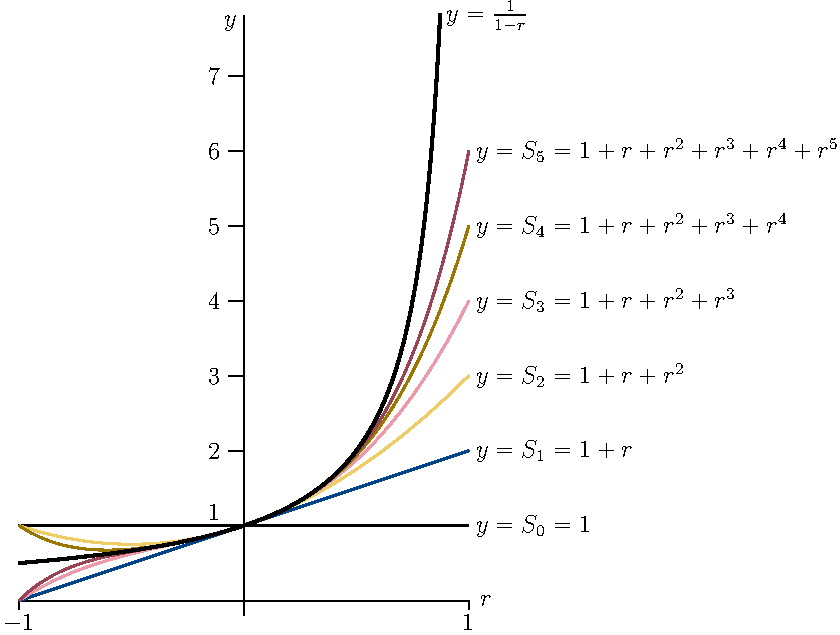
\includegraphics[scale=0.95]{geomT.pdf}
\end{center}
\end{efig}
In these sketches we see that 
\begin{itemize}
\item
when $0< r<1$, and also when $-1<r<0$ with $N$ odd, we have $S_N=\frac{1-r^{N+1}}{1-r}<\frac{1}{1-r}$. On the other hand, when 
$-1<r<0$ with $N$ even, we have $S_N=\frac{1-r^{N+1}}{1-r}>\frac{1}{1-r}$.

\item
When $0< |r|<1$, $S_N=\frac{1-r^{N+1}}{1-r}$ gets closer and closer to $\frac{1}{1-r}$ as $N$ increases.

\item
When $r=-1$, $S_N$ just alternates between $0$, when $N$ is odd, and $1$,
when $N$ is even.
\end{itemize}
\end{eg}
\goodbreak

Now that we know how to handle geometric series let's return to Example~\ref{eg:SRprelimSumA}.
\begin{eg}[Decimal Expansions]\label{eg:SRgeomB}
The decimal expansion
\begin{equation*}
0.3333\cdots
=\frac{3}{10}+\frac{3}{100}+\frac{3}{1000}+\frac{3}{10000}+\cdots
=\sum_{n=1}^\infty\frac{3}{10^n}
\end{equation*}
is a geometric series with the first term $a=\frac{3}{10}$ and the ratio
$r=\frac{1}{10}$. So, by Example \ref{eg:SRgeom},
\begin{equation*}
0.3333\cdots
=\sum_{n=1}^\infty\frac{3}{10^n}
=\frac{\nicefrac{3}{10}}{1-\nicefrac{1}{10}}
=\frac{\nicefrac{3}{10}}{\nicefrac{9}{10}}
=\frac{1}{3}
\end{equation*}
just as we would have expected.

We can push this idea further. Consider the repeating decimal expansion:
\begin{equation*}
0.16161616\cdots
=\frac{16}{100}+\frac{16}{10000}+\frac{16}{1000000}+\cdots
\end{equation*}
This is another geometric series with the first term $a=\frac{16}{100}$
and the ratio $r=\frac{1}{100}$. So, by Example \ref{eg:SRgeom},
\begin{equation*}
0.16161616\cdots
=\sum_{n=1}^\infty\frac{16}{100^n}
=\frac{\nicefrac{16}{100}}{1-\nicefrac{1}{100}}
=\frac{\nicefrac{16}{100}}{\nicefrac{99}{100}}
=\frac{16}{99}
\end{equation*}
again, as expected. In this way any periodic decimal expansion converges
to a ratio of two integers --- that is, to a rational number\footnote{We
have included a (more) formal proof of this fact in the optional
\S \ref{sec:RatIrr}
at the end of this chapter. Proving that a repeating decimal expansion
gives a rational number isn't too hard. Proving the converse --- that
every rational number has a repeating decimal expansion is a
little trickier, but we also do that in the same optional section.}.

Here is another more complicated example.
\begin{align*}
0.1234343434\cdots
&=\frac{12}{100}+\frac{34}{10000}+\frac{34}{1000000}+\cdots \\
%&=\frac{12}{100}+\frac{34}{10000}\Big[1+\frac{1}{100}+\frac{1}{10000}
%         +\cdots\Big] \\
&=\frac{12}{100}+\sum_{n=2}^\infty\frac{34}{100^n} \\
&=\frac{12}{100}+\frac{34}{10000}\frac{1}{1-\nicefrac{1}{100}}
     \quad\text{by Example \ref{eg:SRgeom} with $a=\frac{34}{100^2}$
and $r=\frac{1}{100}$} \\
&=\frac{12}{100}+\frac{34}{10000}\frac{100}{99} \\
&=\frac{1222}{9900}
\end{align*}

\end{eg}

Typically, it is quite difficult to write down a neat closed form
expression for the partial sums of a series.
Geometric series are very notable exceptions to this. Another
family of series for which we can write down partial sums
is called ``telescoping series''. These series have the desirable
property that many of the terms in the sum cancel
each other out rendering the partial sums quite simple.
\begin{eg}[Telescoping Series]\label{eg:SRtelecope}
In this example, we are going to study the series
$\sum_{n=1}^\infty\frac{1}{n(n+1)}$. This is a rather artificial series\footnote{Well\dots this sort of series does
show up when you start to look at the Maclaurin polynomial of functions like $(1-x)\log(1-x)$. So it is not \emph{totally} artificial. At any rate,
it illustrates the basic idea of telescoping very nicely, and the
idea of ``creative telescoping'' turns out to be extremely useful in the
study of series --- though it is well beyond the scope of this course.}
that has been rigged to illustrate a phenomenon called
``telescoping''. Notice that the $n^{\rm th}$ term can be rewritten as
\begin{align*}
\frac{1}{n(n+1)}= \frac{1}{n}-\frac{1}{n+1}
\intertext{and so we have}
a_n &= b_n - b_{n+1} & \text{where } b_n &= \frac{1}{n}.
\end{align*}
Because of this we get big cancellations when we add terms together. This allows us to get a simple formula for the partial sums of this series.
\begin{align*}
S_N&= \frac{1}{1\cdot 2} + \frac{1}{2\cdot 3} + \frac{1}{3\cdot 4} +
          \cdots + \frac{1}{N\cdot (N+1)} \\
&= \Big(\frac{1}{1}-\frac{1}{2}\Big)
  + \Big(\frac{1}{2}-\frac{1}{3}\Big)
  + \Big(\frac{1}{3}-\frac{1}{4}\Big) +
          \cdots + \Big(\frac{1}{N}-\frac{1}{N+1}\Big)
\end{align*}
The second term of each bracket exactly cancels the first term of the following
bracket. So the sum ``telescopes'' leaving just
\begin{equation*}
S_N  = 1-\frac{1}{N+1}
\end{equation*}
and we can now easily compute
\begin{equation*}
\sum_{n=1}^\infty\frac{1}{n(n+1)}
=\lim_{N\rightarrow\infty} S_N
=\lim_{N\rightarrow\infty}\Big( 1-\frac{1}{N+1}\Big)
=1
\end{equation*}
\end{eg}

More generally, if we can write
\begin{align*}
  a_n &= b_n - b_{n+1}
\intertext{%
for some other known sequence $b_n$, then the series telescopes
and we can compute partial sums using}
\sum_{n=1}^N a_n
&=
\sum_{n=1}^N (b_n - b_{n+1}) \\
&=
\sum_{n=1}^N b_n - \sum_{n=1}^N b_{n+1} \\
&= b_1 - b_{N+1}.
\intertext{and hence}
  \sum_{n=1}^\infty a_n
  &= b_1 - \lim_{N\to\infty} b_{N+1}
\end{align*}
provided this limit exists. Often $\lim\limits_{N\to\infty} b_{N+1}=0$
and then $\sum\limits_{n=1}^\infty a_n =b_1$. But this does not always happen.
Here is an example.
\begin{eg}[A Divergent Telescoping Series]\label{eg:SRtelecopeB}
In this example, we are going to study the series
$\sum\limits_{n=1}^\infty\log\big(1+\frac{1}{n}\big)$.
Let's start by just writing out the first few terms.
\begin{alignat*}{5}
\sum_{n=1}^\infty\log\Big(1+\frac{1}{n}\Big)
&=\overbrace{\log\Big(1+\frac{1}{1}\Big)}^{n=1}&&
 +\overbrace{\log\Big(1+\frac{1}{2}\Big)}^{n=2}&&
 +\overbrace{\log\Big(1+\frac{1}{3}\Big)}^{n=3}&&
 +\overbrace{\log\Big(1+\frac{1}{4}\Big)}^{n=4} +\cdots \\
&=\log(2)&&+\log\Big(\frac{3}{2}\Big)&& +\log\Big(\frac{4}{3}\Big)&&
    +\log\Big(\frac{5}{4}\Big) + \cdots
\end{alignat*}
This is pretty suggestive since
\begin{align*}
\log(2)+\log\Big(\frac{3}{2}\Big) +\log\Big(\frac{4}{3}\Big)
+\log\Big(\frac{5}{4}\Big)
=\log\Big(2\times\frac{3}{2}\times\frac{4}{3}\times \frac{5}{4}\Big)
=\log(5)
\end{align*}
So let's try using this idea to compute the partial sum $S_N$:
\begin{alignat*}{5}
S_N&=\sum_{n=1}^N\log\Big(1+\frac{1}{n}\Big)\hidewidth \\
&=\overbrace{\log\Big(1+\frac{1}{1}\Big)}^{n=1}&&
 +\overbrace{\log\Big(1+\frac{1}{2}\Big)}^{n=2}&&
 +\overbrace{\log\Big(1+\frac{1}{3}\Big)}^{n=3}&&+\cdots
 +\overbrace{\log\Big(1+\frac{1}{N-1}\Big)}^{n=N-1}&&
 +\overbrace{\log\Big(1+\frac{1}{N}\Big)}^{n=N}
  \\
&=\log(2)&&+\log\Big(\frac{3}{2}\Big)&& +\log\Big(\frac{4}{3}\Big)&&
    +\cdots+ \log\Big(\frac{N}{N-1}\Big)&&+ \log\Big(\frac{N+1}{N}\Big) \\
&=\log\Big(2\times\frac{3}{2}\times\frac{4}{3}\times \cdots
   \times \frac{N}{N-1}\times \frac{N+1}{N}\Big)\hidewidth
\\
&=\log(N+1)
\end{alignat*}
Uh oh!
\begin{align*}
\lim_{N\rightarrow\infty} S_N
=\lim_{N\rightarrow\infty}\log(N+1)
=+\infty
\end{align*}
This telescoping series diverges!
There is an important lesson here. Telescoping series \emph{can diverge}.
They do not always converge to $b_1$.
\end{eg}

As was the case for limits, differentiation and antidifferentiation,
we can compute more complicated series in
terms of simpler ones by understanding how series interact
with the usual operations of arithmetic. It is, perhaps,
not so surprising that there are simple rules for addition and subtraction
of series and for multiplication of a series by a constant. Unfortunately
there are no simple general rules for computing products or ratios of series.
\begin{theorem}[Arithmetic of series]\label{thm:SRseriesarith}
  Let $A$, $B$ and $C$ be real numbers and let the two series
$\sum_{n=1}^\infty a_n$ and  $\sum_{n=1}^\infty b_n$
converge to $S$ and $T$ respectively. That is, assume that
 \begin{align*}
  \sum_{n=1}^\infty a_n&=S & \sum_{n=1}^\infty b_n &=T
\end{align*}
  Then the following hold.
\begin{enumerate}[(a)]
 \item $\ds \sum_{n=1}^\infty \big[a_n+b_n\big] = S+T\qquad$and
 $\qquad\ds \sum_{n=1}^\infty \big[a_n-b_n\big] = S-T$
      \\
\item $\ds \sum_{n=1}^\infty C a_n = C S$.
\end{enumerate}
\end{theorem}

\begin{eg}\label{eg:SRseriesarith}
As a simple example of how we use the arithmetic of series Theorem
\ref{thm:SRseriesarith}, consider
\begin{equation*}
\sum_{n=1}^\infty\Big[\frac{1}{7^n}+\frac{2}{n(n+1)}\Big]
\end{equation*}
We recognize that we know how to compute parts of this sum.
We know that
\begin{equation*}
\sum_{n=1}^\infty\frac{1}{7^n}=\frac{\nicefrac{1}{7}}{1-\nicefrac{1}{7}}
=\frac{1}{6}
\end{equation*}
because it is a geometric series (Example \ref{eg:SRgeom}) with
first term $a=\frac{1}{7}$ and ratio $r=\frac{1}{7}$. And we
know that
\begin{equation*}
\sum_{n=1}^\infty\frac{1}{n(n+1)} =1
\end{equation*}
by Example \ref{eg:SRtelecope}. We can now use Theorem
\ref{thm:SRseriesarith} to build the specified ``complicated''
series out of these two ``simple'' pieces.
\begin{align*}
\sum_{n=1}^\infty\Big[\frac{1}{7^n}+\frac{2}{n(n+1)}\Big]
&=\sum_{n=1}^\infty \frac{1}{7^n}
   +\sum_{n=1}^\infty\frac{2}{n(n+1)}
 & \text{by Theorem \ref{thm:SRseriesarith}.a} \\
&= \sum_{n=1}^\infty\frac{1}{7^n}
  +2 \sum_{n=1}^\infty \frac{1}{n(n+1)}
 & \text{by Theorem \ref{thm:SRseriesarith}.b} \\
&=\frac{1}{6}+2\cdot 1 =\frac{13}{6}
\end{align*}
\end{eg}


%%%%%%%%%%%%%%%%%%%%%%%%%%%%%
\section{Convergence Tests}
%%%%%%%%%%%%%%%%%%%%%%%%%%%%%

It is very common to encounter series for which it is difficult, or even
virtually impossible, to determine the sum exactly. Often you try to evaluate
the sum approximately by truncating it, i.e. having the index run only
up to some finite $N$, rather than infinity. But there is no point in doing
so if the series diverges\footnote{
The authors should be a little more careful making such a blanket statement. While it is true that it is not wise to approximate a divergent series by taking \(N\) terms with \(N\) large, there are cases when one can get a very good approximation by taking \(N\) terms with \(N\) small! For example, the Taylor remainder theorem shows us that when the \(n^{\rm th}\) derivative of a function \(f(x)\) grows very quickly with \(n\), Taylor polynomials of degree \(N\), with \(N\) large, can give bad approximations of \(f(x)\), while the Taylor polynomials of degree one or two can still provide very good approximations of \(f(x)\) when \(x\) is very small. As an example of this, one of the triumphs of quantum electrodynamics, namely the computation of the anomalous magnetic moment of the electron, depends on precisely this. A number of important quantities were predicted using the first few terms of divergent power series. When those quantities were measured experimentally, the predictions turned out to be incredibly accurate.
}\footnote{
The field of asymptotic analysis often makes use of the first few terms of divergent series to generate approximate solutions to problems; this, along with numerical computations, is one of the most important techniques in applied mathematics. Indeed, there is a whole wonderful book  (which, unfortunately, is too advanced for most Calculus~2 students) devoted to playing with divergent series called, unsurprisingly, ``Divergent Series'' by G.H.~Hardy. This is not to be confused with the ``Divergent'' series by V.~Roth set in a post-apocalyptic dystopian Chicago. That latter series diverges quite dramatically from mathematical topics, while the former does not have a film adaptation (yet).
}. So you like to at least know if the series converges
or diverges. Furthermore you would also like to know what error is introduced
when you approximate $\sum_{n=1}^\infty a_n$ by the ``truncated series''
$\sum_{n=1}^Na_n$. That's called the truncation error. There are a number
of ``convergence tests'' to help you with this.
\begin{comment}
Note from Joel to Joel:  By an argument of Dyson (F.J. Dyson, Divergence of perturbation theory in quantum electrodynamics,Phys. Rev.,85, 631-632 (1952))
perturbation expansions in QED cannot be anaytic at $e=0$ because if $e^2<0$
the vacuum will be unstable.
\end{comment}

%%%%%%%%%%%%%%%%%%%%%%%%%%%%%
\subsection{The Divergence Test}
%%%%%%%%%%%%%%%%%%%%%%%%%%%%%

Our first test is very easy to apply, but it is also rarely useful.
It just allows us to quickly reject some ``trivially divergent'' series.
It is based on the observation that
\begin{itemize}
\item  by definition, a series $\sum_{n=1}^\infty a_n$
converges to $S$ when the partial sums $S_N=\sum_{n=1}^N a_n$ converge
to  $S$.
\item Then, as $N\rightarrow\infty$, we have $S_N\rightarrow S$ and,
because $N-1\rightarrow\infty$ too, we also have $S_{N-1}\rightarrow S$.
\item
So $a_N=S_N-S_{N-1}\rightarrow S-S=0$.
\end{itemize}
This tells us that, if we already know that a given series $\sum a_n$
is convergent, then the $n^{\rm th}$ term of the series, $a_n$,
must converge to $0$ as $n$ tends to infinity. In this form,
the test is not so useful. However the
contrapositive\footnote{We have discussed the contrapositive a few times
in the CLP notes, but it doesn't hurt to discuss it again here (or for
the reader to quickly look up the relevant footnote in Section 1.3 of
the CLP-1 text).
At any rate, given a statement of the form ``If A is true, then B is true''
the contrapositive is ``If B is not true, then A is not true''.
The two statements in quotation marks are logically equivalent ---
if one is true, then so is the other. In the present context we have
\begin{quote}
 If \ \ ($\sum a_n$ converges)\ \  then \ \ ($a_n$ converges to $0$).
\end{quote}
The contrapositive of this statement is then
\begin{quote}
 If  \ \ ($a_n$ does not converge to 0)\ \  then
   \ \ ($\sum a_n$ does not converge).
\end{quote}
} of the statement is a useful test for \emph{divergence}.

\begin{theorem}[Divergence Test]\label{thm:SRdivergenceTest}
If the sequence $\big\{a_n\big\}_{n=1}^\infty$ fails to converge to zero
as $n\rightarrow\infty$, then the series $\sum_{n=1}^\infty a_n$ diverges.
\end{theorem}

\begin{eg}\label{eg:SRdivTest}
Let $a_n=\frac{n}{n+1}$. Then
\begin{equation*}
\lim_{n\rightarrow\infty} a_n
=\lim_{n\rightarrow\infty}\frac{n}{n+1}
=\lim_{n\rightarrow\infty}\frac{1}{1+\nicefrac{1}{n}}
=1\ne 0
\end{equation*}
So the series $\sum_{n=1}^\infty \frac{n}{n+1}$ diverges.

\end{eg}

\begin{warning}\label{wrn:SRdivTest}
The divergence test is a ``one way test''. It tells us that if
$\lim_{n\rightarrow\infty}a_n$ is nonzero, or fails to exist, then
the series $\sum_{n=1}^\infty a_n$ diverges. But it tells us \emph{absolutely
nothing} when $\lim_{n\rightarrow\infty}a_n=0$. In particular, it is perfectly
possible for a series $\sum_{n=1}^\infty a_n$ to \emph{diverge} even
though  $\lim_{n\rightarrow\infty}a_n=0$.
An example is $\sum_{n=1}^\infty \frac{1}{n}$. We'll show in Example
\ref{eg:SRpTest}, below, that it diverges.
\end{warning}


Now while convergence or divergence of series like
$\sum_{n=1}^\infty \frac{1}{n}$ can be determined using some
clever tricks --- see the optional \S\ref{sec:HarminicBasel} ---,
it would be much better to have methods that are more systematic and
rely less on being sneaky. Over the next subsections we will discuss
several methods for testing series for convergence.


Note that while these tests will tell us whether or not a series
converges, they do not (except in rare cases) tell us what the
series adds up to. For example, the test we will
see in the next subsection tells us quite immediately that the series
\begin{align*}
  \sum_{n=1}^\infty \frac{1}{n^3}
\end{align*}
converges. However it does not tell us its value\footnote{This series
converges to Ap\'ery's constant $1.2020569031\dots$. The constant is
named for Roger Ap\'ery (1916--1994) who proved that this number must be irrational. This number appears in many contexts including the following
cute fact --- the reciprocal of Ap\'ery's constant gives the probability
that three positive integers, chosen at random, do not share
a common prime factor.}.


%%%%%%%%%%%%%%%%%%%%%%%%%%%%%
\subsection{The Integral Test}
%%%%%%%%%%%%%%%%%%%%%%%%%%%%%

In the integral test, we think of a series $\sum_{n=1}^\infty a_n$, that
we cannot evaluate explicitly, as the area of a union of rectangles,
with $a_n$ representing the area of a rectangle of width one and
height $a_n$. Then we compare that area with the area represented
by an integral, that we can evaluate explicitly, much as we did in
Theorem \ref{thm:IMPcomparison}, the comparison test for improper integrals.
We'll start with a simple example,  to illustrate the idea.
Then we'll move on to a formulation of the test in general.

\begin{eg}\label{eg:firstIntTest}
Visualise the terms of the harmonic series $\sum_{n=1}^\infty\frac{1}{n}$
as a bar graph --- each term is a rectangle of
height $\frac{1}{n}$ and width $1$. The limit of the series is then the limiting area of this union of rectangles. Consider the sketch
on the left below.
\begin{wfig}
 \begin{center}
  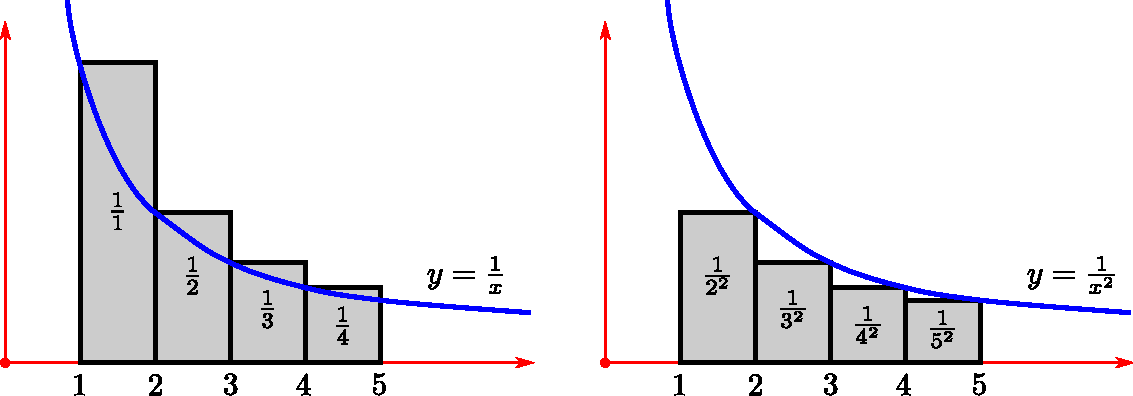
\includegraphics[height=5cm]{harmonic_int.pdf}
 \end{center}
\end{wfig}
It shows that the area of the shaded columns, $\sum_{n=1}^4\frac{1}{n}$,
is bigger than the area under the curve $y=\frac{1}{x}$ with
$1\le x\le 5$. That is
\begin{align*}
  \sum_{n=1}^4 \frac{1}{n}
  & \ge \int_1^5 \frac{1}{x}\dee{x}
\end{align*}
If we were to continue drawing the columns all the way out to infinity,
then we would have
\begin{align*}
  \sum_{n=1}^\infty \frac{1}{n}
  & \ge \int_1^\infty \frac{1}{x}\dee{x}
\end{align*}
We are able to compute this improper integral exactly:
\begin{align*}
  \int_1^\infty \frac{1}{x} \dee{x}
  &= \lim_{R \to \infty} \Big[ \log|x| \Big]_1^R
  = +\infty
\end{align*}
That is the area under the curve diverges to $+\infty$ and so the area represented by the columns must also diverge to
$+\infty$.

It should be clear that the above argument can be quite easily
generalised. For example the same argument holds
\emph{mutatis mutandis}\footnote{Latin for ``Once the necessary changes
are made''. This phrase still gets used a little, but
these days mathematicians tend to write something equivalent in English. Indeed, English is pretty much the \emph{lingua franca} for
mathematical publishing. \emph{Quidquid erit.}} for the series
\begin{align*}
  \sum_{n=1}^\infty \frac{1}{n^2}
\end{align*}
Indeed we see from the sketch on the right above that
\begin{align*}
  \sum_{n=2}^N \frac{1}{n^2}
  &\le \int_1^N \frac{1}{x^2}\dee{x}
\end{align*}
and hence
\begin{align*}
  \sum_{n=2}^\infty \frac{1}{n^2}
   \leq \int_1^\infty \frac{1}{x^2}\dee{x}
\end{align*}
This last improper integral is easy to evaluate:
\begin{align*}
  \int_1^\infty \frac{1}{x^2}\dee{x}
  &= \lim_{R\to\infty} \left[ - \frac{1}{x} \right]_1^R \\
  &= \lim_{R\to\infty} \left( \frac{1}{1} - \frac{1}{R} \right)
  = 1
\end{align*}
Thus we know that
\begin{align*}
  \sum_{n=1}^\infty \frac{1}{n^2}
 = 1+ \sum_{n=2}^\infty \frac{1}{n^2} \leq 2.
\end{align*}
and so the series must converge.
\end{eg}


The above arguments are formalised in the following theorem.
\begin{theorem}[The Integral Test]\label{thm:SRintegralTest}
Let $N_0$ be any natural number. If $f(x)$ is a function which is defined
and continuous for all $x\ge N_0$ and which obeys
\begin{enumerate}[(i)]\itemsep1pt \parskip0pt \parsep0pt %\itemindent-15pt
\item $f(x)\ge 0$ for all $x\ge N_0$ and
\item $f(x)$ decreases as $x$ increases and
\item $f(n)=a_n$ for all  $n\ge N_0$.
\end{enumerate}
%\begin{efig}
\begin{center}
   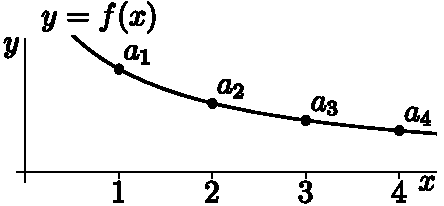
\includegraphics{intTest}
\end{center}
%\end{efig}
Then
\begin{equation*}
\sum_{n=1}^\infty a_n\text{ converges }\iff
\int_{N_0}^\infty f(x)\ \dee{x}\text{ converges}
\end{equation*}
Furthermore, when the series converges, the truncation error
\begin{equation*}
\bigg|\sum_{n=1}^\infty a_n-\sum_{n=1}^N a_n\bigg|\le
  \int_N^\infty f(x)\ \dee{x}\qquad\text{for all $N\ge N_0$}
\end{equation*}
\end{theorem}

\begin{proof}
Let $I$ be any fixed integer with $I>N_0$. Then
\begin{itemize}
\item
$\sum_{n=1}^\infty a_n$ converges if and only if
$\sum_{n=I}^\infty a_n$ converges --- removing a fixed finite number
of terms from a series cannot impact whether or not it converges.
\item
Since $a_n\ge 0$ for all $n\ge I>N_0$, the sequence of partial sums
$s_\ell=\sum_{n=I}^\ell a_n$ obeys $s_{\ell+1} = s_\ell+a_{n+1}
\ge s_\ell$. That is, $s_\ell$ increases as $\ell$ increases.
\item
So $\big\{s_\ell\big\}$ must either
converge to some finite number or increase to infinity. That is, either
$\sum_{n=I}^\infty a_n$ converges to a finite number or it is $+\infty$.
\end{itemize}
\begin{efig}
\begin{center}
     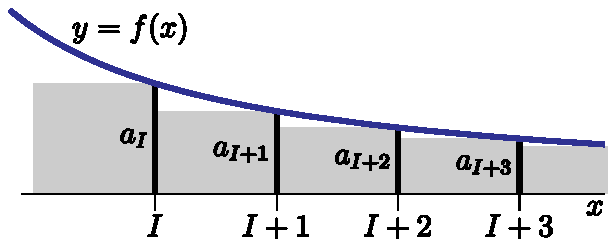
\includegraphics{intTest3.pdf}
\end{center}
\end{efig}

Look at the figure above. The shaded area in the figure is
$\sum_{n=I}^\infty a_n$ because
\begin{itemize}\itemsep1pt \parskip0pt \parsep0pt %\itemindent-15pt
\item the first shaded rectangle has height $a_I$
and width $1$, and hence area $a_I$ and
\item the second shaded rectangle has height $a_{I+1}$
and width $1$, and hence area $a_{I+1}$, and so on
\end{itemize}
This shaded area is smaller than the area under the curve $y=f(x)$ for
$I-1\le x<\infty$. So
\begin{equation*}
\sum_{n=I}^\infty a_n
\le \int_{I-1}^\infty f(x)\ \dee{x}
\end{equation*}
and, if the integral is finite, the sum $\sum_{n=I}^\infty a_n$ is
finite too.
Furthermore, the desired bound on the truncation error is just
the special case of this inequality with $I=N+1$:
\begin{align*}
\sum_{n=1}^\infty a_n - \sum_{n=1}^N a_n
=\sum_{n=N+1}^\infty a_n
\le \int_N^\infty f(x)\ \dee{x}
\end{align*}


\begin{efig}
\begin{center}
     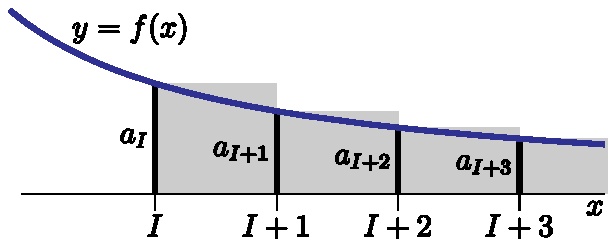
\includegraphics{intTest4.pdf}
\end{center}
\end{efig}

For the ``divergence case'' look at the figure above.
The (new) shaded area in the figure is again $\sum_{n=I}^\infty a_n$
because
\begin{itemize}\itemsep1pt \parskip0pt \parsep0pt %\itemindent-15pt
\item the first shaded rectangle has height $a_I$
and width $1$, and hence area $a_I$ and
\item the second shaded rectangle has height $a_{I+1}$
and width $1$, and hence area $a_{I+1}$, and so on
\end{itemize}
This time the shaded area is larger than the area under the curve
$y=f(x)$ for $I\le x<\infty$. So
\begin{equation*}
\sum_{n=I}^\infty a_n
\ge \int_I^\infty f(x)\ \dee{x}
\end{equation*}
and, if the integral is infinite, the sum $\sum_{n=I}^\infty a_n$ is infinite
too.


\end{proof}

Now that we have the integral test, it is straightforward to determine
for which values of $p$ the series\footnote{This series, viewed
as a function of $p$, is called the Riemann zeta function, $\zeta(p)$,
or the Euler-Riemann zeta function. It is extremely important because
of its connections to prime numbers (among many other things). Indeed
Euler proved that
\begin{align*}
\zeta(p) = \sum_{n=1}^\infty \frac{1}{n^p}
           &= \prod_{\text{P prime}} \left(1 - {\rm P}^{-p} \right)^{-1}
\end{align*}
Riemann showed the connections between the zeros of this function (over
complex numbers $p$) and the distribution of prime numbers. Arguably the
most famous unsolved problem in mathematics, the Riemann
hypothesis, concerns the locations of zeros of this function.
}
\begin{align*}
 \sum_{n=1}^\infty \frac{1}{n^p}
\end{align*}
converges.


\begin{eg}[The $p$ test:  $\sum\limits_{n=1}^\infty\frac{1}{n^p}$]
                                                    \label{eg:SRpTest}
Let $p>0$. We'll now use the integral test to determine whether or not the
series $\sum_{n=1}^\infty\frac{1}{n^p}$ (which is sometimes called
the $p$--series) converges.
\begin{itemize}
\item To do so, we
need a function $f(x)$ that obeys $f(n)=a_n=\frac{1}{n^p}$ for all $n$
bigger than some $N_0$. Certainly $f(x)=\frac{1}{x^p}$ obeys
$f(n)=\frac{1}{n^p}$ for all $n\ge 1$. So let's pick this $f$ and try $N_0=1$.
(We can always increase $N_0$ later if we need to.)
\item
This function also obeys the other two conditions of
Theorem \ref{thm:SRintegralTest}:
\begin{enumerate}[(i)]
\item $f(x)>0$ for all $x\ge N_0=1$ and
\item $f(x)$ decreases as $x$ increases because $f'(x)=-p\frac{1}{x^{p+1}}<0$
for all $x\ge N_0=1$.
\end{enumerate}
\item
So the integral test tells us that the series
$\sum_{n=1}^\infty\frac{1}{n^p}$ converges if and only if the integral
$\int_1^\infty\frac{\dee{x}}{x^p}$ converges.
\item
We have already seen, in Example \ref{eg:IMPp1}, that
the integral $\int_1^\infty\frac{\dee{x}}{x^p}$ converges if and only if $p>1$.
\end{itemize}
So we conclude that $\sum_{n=1}^\infty\frac{1}{n^p}$ converges if
and only if $p>1$. This is sometimes called the $p$--test.
\begin{itemize}
\item
In particular, the series $\sum_{n=1}^\infty\frac{1}{n}$,
which is called the harmonic series, has $p=1$ and so diverges.
As we add more and more terms of this series together, the terms we add,
namely $\frac{1}{n}$, get smaller and smaller and tend to zero,
%but the \emph{rate} at which they tend to zero is small enough
but they tend to zero so slowly
that the full sum is still infinite.
\item
On the other hand, the series $\sum_{n=1}^\infty\frac{1}{n^{1.000001}}$ has
$p = 1.000001>1$ and so converges. This time as we add more and more
terms of this series together, the terms we add, namely
$\frac{1}{n^{1.000001}}$, tend to zero (just) fast enough that
the full sum is finite. Mind you, for this example, the
convergence takes place very slowly --- you have to take a huge number
of terms to get a decent approximation to the full sum.
If we approximate $\sum_{n=1}^\infty\frac{1}{n^{1.000001}}$ by the
truncated series $\sum_{n=1}^N\frac{1}{n^{1.000001}}$, we make an error of
at most
\begin{align*}
\int_N^\infty \frac{\dee{x}}{x^{1.000001}}
= \lim_{R\rightarrow\infty} \int_N^R \frac{\dee{x}}{x^{1.000001}}
= \lim_{R\rightarrow\infty}- \frac{1}{0.000001}
          \Big[\frac{1}{R^{0.000001}}-\frac{1}{N^{0.000001}}\Big]
=\frac{10^6}{N^{0.000001}}
\end{align*}
This does tend to zero as $N\rightarrow\infty$, but really slowly.
\end{itemize}
\end{eg}
\goodbreak

We now know that the dividing line between convergence and divergence
of $\sum_{n=1}^\infty\frac{1}{n^p}$ occurs at $p=1$. We can dig
a little deeper and ask ourselves how much more quickly than
$\frac{1}{n}$ the $n^{\rm th}$ term
needs to shrink in order for the series to converge.
We know that for large $x$, the function $\log x$ is smaller than
$x^a$ for any positive $a$ --- you can convince yourself of this with
a quick application of L'H\^opital's rule. So it is not unreasonable
to ask whether the series
\begin{align*}
  \sum_{n=2}^\infty \frac{1}{n \log n}
\end{align*}
converges. Notice that we sum from $n=2$ because when $n=1, n\log n=0$.
And we don't need to stop there\footnote{We could go even further and see
what happens if we include powers of $\log(\log(n))$ and other more
exotic slow growing functions.}. We can analyse the convergence of
this sum with any power of $\log n$.


\begin{eg}[$\sum\limits_{n=2}^\infty\frac{1}{n(\log n)^p}$]\label{eg:SRlnpTest}
Let $p>0$. We'll now use the integral test to determine whether or not the
series $\sum\limits_{n=2}^\infty\frac{1}{n(\log n)^p}$ converges.
\begin{itemize}
\item
As in the last example, we start by choosing a function that obeys
$f(n)=a_n=\frac{1}{n(\log n)^p}$ for all $n$
bigger than some $N_0$. Certainly $f(x)=\frac{1}{x(\log x)^p}$ obeys
$f(n)=\frac{1}{n(\log n)^p}$ for all $n\ge 2$. So let's use that $f$ and
try $N_0=2$.
\item
Now let's check the other two conditions of
Theorem \ref{thm:SRintegralTest}:
\begin{enumerate}[(i)]
\item Both $x$ and $\log x$ are positive for all $x>1$, so $f(x)>0$ for all $x\ge N_0=2$.
\item  As $x$ increases both $x$ and $\log x$ increase and so $x(\log x)^p$
increases and $f(x)$ decreases.
\end{enumerate}
\item
So the integral test tells us that the series
$\sum\limits_{n=2}^\infty\frac{1}{n(\log n)^p}$ converges if and only if
the integral $\int_2^\infty\frac{\dee{x}}{x (\log x)^p}$ converges.
\item
To test
the convergence of the integral, we make the substitution $u=\log x$,
$\dee{u}=\frac{\dee{x}}{x}$.
\begin{align*}
\int_2^R \frac{\dee{x}}{x (\log x)^p}
=\int_{\log 2}^{\log R}\frac{\dee{u}}{u^p}
\end{align*}
 We already know that the integral $\int_1^\infty\frac{\dee{u}}{u^p}$,
and hence the integral $\int_2^R \frac{\dee{x}}{x (\log x)^p}$, converges if and
only if $p>1$.
\end{itemize}
So we conclude that
$\sum\limits_{n=2}^\infty\frac{1}{n(\log n)^p}$
converges if and only if $p>1$.
\end{eg}

%%%%%%%%%%%%%%%%%%%%%%%%%%%%%
\subsection{The Comparison Test}
%%%%%%%%%%%%%%%%%%%%%%%%%%%%%

Our next convergence test is the comparison test. It is much like
the comparison test for improper integrals (see Theorem \ref{thm:IMPcomparison})
and is true for much the same reasons.
The rough idea is quite simple. A sum of larger terms
must be bigger than a sum of smaller terms. So if we know the
big sum converges, then the small sum must converge too. On the other
hand, if we know the small sum diverges, then the big sum must also
diverge. Formalising this idea gives the following theorem.
\begin{theorem}[The Comparison Test]\label{thm:SRcomparisonTest}
Let $N_0$ be a natural number and let $K>0$.
\begin{enumerate}[(a)]
\item If $|a_n|\le K c_n$ for all $n\ge N_0$ and
$\sum\limits_{n=0}^\infty c_n$ converges, then
$\sum\limits_{n=0}^\infty a_n$ converges.
\item If $a_n\ge K d_n\ge0 $ for all $n\ge N_0$ and
$\sum\limits_{n=0}^\infty d_n$ diverges, then
$\sum\limits_{n=0}^\infty a_n$ diverges.
\end{enumerate}
\end{theorem}

\begin{proof}[``Proof'']
We will not prove this theorem here. We'll just observe that it is very
reasonable. That's why there are quotation marks around ``Proof''.
For an actual proof see the optional section \ref{sec:CompProof}.
\begin{enumerate}[(a)]
\item If $\sum\limits_{n=0}^\infty c_n$ converges to a finite number
and if the terms in $\sum\limits_{n=0}^\infty a_n$ are smaller than the
terms in $\sum\limits_{n=0}^\infty c_n$, then it is no surprise that
$\sum\limits_{n=0}^\infty a_n$ converges too.

\item If $\sum\limits_{n=0}^\infty d_n$ diverges (i.e. adds up to $\infty$)
and if the terms in $\sum\limits_{n=0}^\infty a_n$ are larger than the
terms in $\sum\limits_{n=0}^\infty d_n$, then of course
$\sum\limits_{n=0}^\infty a_n$ adds up to $\infty$, and so diverges, too.
\end{enumerate}

\end{proof}

The comparison test for series is also used in much the same way as is
the comparison test for improper integrals. Of course, one needs a good
series to compare against, and often the series $\sum n^{-p}$ (from Example~\ref{eg:SRpTest}), for some $p>0$, turns out to be just
what is needed.

\goodbreak
\begin{eg}[$\sum_{n=1}^\infty\frac{1}{n^2+2n+3}$]\label{eg:SRcomparisonTestA}
We could determine whether or not the series $\sum_{n=1}^\infty\frac{1}{n^2+2n+3}$
converges by applying the integral test. But it is not worth the effort\footnote{Go back and quickly scan
Theorem~\ref{thm:SRintegralTest}; to apply it we need to show that
$\frac{1}{n^2+2n+3}$ is  positive and decreasing (it is), and then
we need to integrate $\int \frac{1}{x^2+2x+3}\dee{x}$. To do that
we reread the notes on partial fractions, then rewrite $x^2+2x+3
= (x+1)^2+2$ and so
\begin{align*}
  \int_1^\infty \frac{1}{x^2+2x+3}\dee{x}
  &= \int_1^\infty \frac{1}{(x+1)^2+2}\dee{x} \cdots
\end{align*}
and then arctangent appears,  etc etc. Urgh. Okay --- let's go
back to the text now and see how to avoid this.
}.
Whether or not any series converges is determined by the behaviour
of the summand\footnote{To understand this consider any series
$\sum_{n=1}^\infty a_n$. We can always cut such a series into
two parts --- pick some huge number like $10^6$. Then
\begin{align*}
\sum_{n=1}^\infty a_n
&= \sum_{n=1}^{10^6} a_n + \sum_{n=10^6+1}^\infty a_n
\end{align*}
The first sum, though it could be humongous, is finite. So
the left hand side, $\sum_{n=1}^\infty a_n$, is a well--defined finite
number if and only if $\sum_{n=10^6+1}^\infty a_n$, is a well--defined
finite number. The convergence or divergence of the series is
determined by the second sum, which  only contains $a_n$ for ``large'' $n$.}
for very large $n$. So the first step in tackling such
a problem is to develop some intuition about the behaviour of $a_n$ when
$n$ is very large.
\begin{itemize}
\item \emph{Step 1: Develop intuition.}\ \ \
In this case, when $n$ is very large\footnote{The symbol ``$\gg$''
means ``much larger than''. Similarly, the symbol ``$\ll$'' means ``much
less than''. Good shorthand symbols can be quite expressive.}
$n^2\gg 2n \gg 3$ so that  $\frac{1}{n^2+2n+3}\approx\frac{1}{n^2}$.
We already know, from Example \ref{eg:SRpTest}, that
$\sum_{n=1}^\infty\frac{1}{n^p}$ converges if and only if $p>1$.
So $\sum_{n=1}^\infty\frac{1}{n^2}$, which has $p=2$, converges, and
we would expect that
$\sum_{n=1}^\infty\frac{1}{n^2+2n+3}$ converges too.
\item \emph{Step 2: Verify intuition.}\ \ \
We can use the comparison test to confirm that this is indeed the case.
For any $n\ge 1$, $n^2+2n+3 > n^2$, so that
$\frac{1}{n^2+2n+3}\le\frac{1}{n^2}$. So the comparison test,
Theorem \ref{thm:SRcomparisonTest}, with $a_n=\frac{1}{n^2+2n+3}$ and
$c_n=\frac{1}{n^2}$, tells us that $\sum_{n=1}^\infty\frac{1}{n^2+2n+3}$
converges.
\end{itemize}
\end{eg}

Of course the previous example was ``rigged'' to give an easy application
of the comparison test. It is often relatively easy, using arguments like
those in Example \ref{eg:SRcomparisonTestA}, to find a
``simple'' series $\sum_{n=1}^\infty b_n$ with $b_n$ almost the same
as $a_n$ when $n$ is large. However it is pretty rare that $a_n\le b_n$
for all $n$. It is much more common that $a_n\le K b_n$
for some constant $K$. This is enough to allow application of the
comparison test. Here is an example.

\begin{eg}[$\sum_{n=1}^\infty\frac{n+\cos n}{n^3-1/3}$]
                                   \label{eg:SRcomparisonTestB}
As in the previous example, the first step is to develop some
intuition about the behaviour of $a_n$ when $n$ is very large.
\begin{itemize}
\item \emph{Step 1: Develop intuition.}\ \ \
When $n$ is very large,
\begin{itemize}
\item[$\circ$] $n\gg |\cos n|$ so that  the numerator $n+\cos n\approx n$  and
\item[$\circ$] $n^3 \gg \nicefrac{1}{3}$ so that the denominator
$n^3-\nicefrac{1}{3}\approx n^3$.
\end{itemize}
So when $n$ is very large
\begin{equation*}
a_n=\frac{n+\cos n}{n^3-\nicefrac{1}{3}}\approx\frac{n}{n^3}=\frac{1}{n^2}
\end{equation*}
We already know from Example \ref{eg:SRpTest}, with $p=2$, that
$\sum_{n=1}^\infty\frac{1}{n^2}$ converges, so we would expect that
$\sum_{n=1}^\infty\frac{n+\cos n}{n^3-\nicefrac{1}{3}}$ converges too.
\item \emph{Step 2: Verify intuition.}\ \ \
We can use the comparison test to confirm that this is indeed the case.
To do so we need to find a constant $K$ such that  $|a_n|=
\frac{|n+\cos n|}{n^3-1/3}=\frac{n+\cos n}{n^3-1/3}$
is smaller than $\frac{K}{n^2}$ for all $n$. A good way\footnote{This is very similar to how we computed limits at infinity way way back near the
beginning of CLP-1.} to do
that is to factor the dominant term (in this case $n$) out of the
numerator and also factor the dominant term (in this case $n^3$)
out of the denominator.
\begin{equation*}
a_n=\frac{n+\cos n}{n^3-\nicefrac{1}{3}}
=\frac{n}{n^3}\
   \frac{1+\frac{\cos n}{n}}{1-\frac{1}{3n^3}}
=\frac{1}{n^2}\
   \frac{1+\frac{\cos n}{n}}{1-\frac{1}{3n^3}}
\end{equation*}
So now we need to find a constant $K$ such that
$\frac{1+\nicefrac{(\cos n)}{n}}{1-\nicefrac{1}{3n^3}}$
is smaller than $K$ for all $n\ge 1$.
\begin{itemize}
\item[$\circ$]
First consider the numerator $1+(\cos n)\frac{1}{n}$.
For all $n\ge 1$
\begin{itemize}
\item $\frac{1}{n}\le 1$ and
\item $|\cos n|\le 1$
\end{itemize}
So the numerator $1+(\cos n)\frac{1}{n}$
is always smaller than $1+(1)\frac{1}{1}=2$.
\item[$\circ$]
Next consider the denominator $1-\nicefrac{1}{3n^3}$.
\begin{itemize}
\item
When $n\ge 1$, $\frac{1}{3n^3}$ lies between $\frac{1}{3}$ and $0$
so that
\item
$1-\frac{1}{3n^3}$ is between $\frac{2}{3}$ and $1$ and consequently
\item
$\frac{1}{1-\nicefrac{1}{3n^3}}$
is between $\frac{3}{2}$ and $1$.
\end{itemize}
\item[$\circ$] As the numerator $1+(\cos n)\frac{1}{n}$ is always smaller
than $2$ and $\frac{1}{1-\nicefrac{1}{3n^3}}$
is always smaller than $\frac{3}{2}$, the fraction
\begin{equation*}
\frac{1+\frac{\cos n}{n}}{1-\frac{1}{3n^3}}
\le 2\Big(\frac{3}{2}\Big)
=3
\end{equation*}
\end{itemize}
We now know that
\begin{equation*}
|a_n| =\frac{1}{n^2}\
   \frac{1+\nicefrac{2}{n}}{1-\nicefrac{1}{3n^3}}
\le  \frac{3}{n^2}
\end{equation*}
and, since we know $\sum_{n=1}^\infty n^{-2}$ converges,
the comparison test tells us that
$\sum_{n=1}^\infty\frac{n+\cos n}{n^3-1/3}$ converges.
\end{itemize}
\end{eg}

The last example was actually a relatively simple application of the comparison theorem --- finding a suitable constant
$K$ can be \emph{really} tedious\footnote{Really, really tedious. And you thought some of those partial fractions
computations were bad \dots}. Fortunately, there is a variant of the
comparison test that completely eliminates the need to explicitly
find $K$.

The idea behind this isn't too complicated. We have already seen
that the convergence or divergence of a series depends not on its
first few terms, but just on what happens when $n$ is really large.
Consequently, if we can work out how  the series terms behave for
really big $n$ then we can work out if the series converges.
So instead of comparing the terms of our series for all $n$, just
compare them when $n$ is big.
\begin{theorem}[Limit Comparison Theorem]\label{thm:SRlimitComparison}
Let $\sum_{n=1}^\infty a_n$ and $\sum_{n=1}^\infty b_n$ be two series with
$b_n>0$ for all $n$. Assume that
\begin{equation*}
\lim_{n\rightarrow\infty}\frac{a_n}{b_n}=L
\end{equation*}
exists.
\begin{enumerate}[(a)]
\item If $\sum_{n=1}^\infty b_n$  converges, then
$\sum_{n=1}^\infty a_n$ converges too.

\item If $L\ne 0$ and $\sum_{n=1}^\infty b_n$  diverges,
then $\sum_{n=1}^\infty a_n$ diverges too.
\end{enumerate}
In particular, if $L\ne 0$, then $\sum_{n=1}^\infty a_n$ converges
if and only if $\sum_{n=1}^\infty b_n$ converges.

\end{theorem}

\begin{proof} (a)\ \ \
Because we are told that
$
\lim_{n\rightarrow\infty}\frac{a_n}{b_n}=L
$,
we know that,
\begin{itemize}
\item
when $n$ is large,  $\frac{a_n}{b_n}$ is very close to $L$,
so that $\Big|\frac{a_n}{b_n}\Big|$ is very close to $|L|$.
\item
In particular, there is some natural number $N_0$ so that
$\Big|\frac{a_n}{b_n}\Big|\le |L|+1$, for all $n\ge N_0$, and hence
\item
$|a_n|\le Kb_n$ with $K=|L|+1$, for all $n\ge N_0$.
\item
The comparison Theorem \ref{thm:SRcomparisonTest}
now implies that $\sum_{n=1}^\infty a_n$ converges.
\end{itemize}


\noindent (b)\ \ \
 Let's suppose that $L>0$. (If $L<0$, just replace $a_n$
with $-a_n$.) Because we are told that
$
\lim_{n\rightarrow\infty}\frac{a_n}{b_n}=L
$,
we know that,
\begin{itemize}
\item
when $n$ is large,  $\frac{a_n}{b_n}$ is very close to $L$.
\item
In particular, there is some natural number $N$ so that
$\frac{a_n}{b_n}\ge \frac{L}{2}$, and hence
\item
$a_n\ge Kb_n$ with $K=\frac{L}{2}>0$, for all $n\ge N$.
\item
The comparison Theorem \ref{thm:SRcomparisonTest}
now implies that $\sum_{n=1}^\infty a_n$ diverges.
\end{itemize}
\end{proof}

The next two examples illustrate how much of an improvement the above
theorem is over the straight comparison test (though of course, we
needed the comparison test to develop the limit comparison test).
\begin{eg}[$\sum_{n=1}^\infty\frac{\sqrt{n+1}}{n^2-2n+3}$]\label{eg:SRlimCompA}
Set $a_n= \frac{\sqrt{n+1}}{n^2-2n+3}$.  We first try to develop some
intuition about the behaviour of $a_n$ for large $n$ and then we confirm
that our intuition was correct.
\begin{itemize}
\item \emph{Step 1: Develop intuition.}\ \ \
When $n\gg 1$,
the numerator $\sqrt{n+1}\approx \sqrt{n}$, and the denominator
$n^2-2n+3\approx n^2$ so that
$a_n\approx \frac{\sqrt{n}}{n^2}=\frac{1}{n^{3/2}}$ and it looks like
our series should converge by Example \ref{eg:SRpTest} with $p=\frac{3}{2}$.

\item \emph{Step 2: Verify intuition.}\ \ \
To confirm our intuition we set $b_n=\frac{1}{n^{3/2}}$ and
compute the limit
\begin{equation*}
\lim_{n\rightarrow\infty}\frac{a_n}{b_n}
=\lim_{n\rightarrow\infty}\frac{\frac{\sqrt{n+1}}{n^2-2n+3}}{\frac{1}{n^{3/2}}}
=\lim_{n\rightarrow\infty}\frac{n^{3/2}\sqrt{n+1}}{n^2-2n+3}
\end{equation*}
Again it is a good idea to factor the dominant term out of the
numerator and the dominant term out of the denominator.
\begin{equation*}
\lim_{n\rightarrow\infty}\frac{a_n}{b_n}
=\lim_{n\rightarrow\infty}\frac{n^2\sqrt{1+\nicefrac{1}{n}}}
                {n^2\big(1-\nicefrac{2}{n}+\nicefrac{3}{n^2}\big)}
=\lim_{n\rightarrow\infty}\frac{\sqrt{1+\nicefrac{1}{n}}}
           {1-\nicefrac{2}{n}+\nicefrac{3}{n^2}}
=1
\end{equation*}
We already know that the series $\sum_{n=1}^\infty b_n
=\sum_{n=1}^\infty\frac{1}{n^{3/2}}$ converges by
Example \ref{eg:SRpTest} with $p=\frac{3}{2}$.
So our series converges by the limit comparison test,
Theorem \ref{thm:SRlimitComparison}.
\end{itemize}
\end{eg}

\begin{eg}[$\sum_{n=1}^\infty\frac{\sqrt{n+1}}{n^2-2n+3}$, again]
          \label{eg:SRlimCompAbis}
We can also try to deal with the series of Example \ref{eg:SRlimCompA},
using the comparison test directly.
But that requires us to find $K$ so that
\begin{align*}
  \frac{\sqrt{n+1}}{n^2-2n+3} & \leq \frac{K}{n^{3/2}}
\end{align*}
We might do this by examining the numerator and denominator separately:
\begin{itemize}
 \item The numerator isn't too bad since for all $n \geq 1$:
 \begin{align*}
  n+1 &\leq 2n \qquad \text{and so}\\
  \sqrt{n+1} &\leq \sqrt{2n}
\end{align*}
\item The denominator is quite a bit more tricky, since we need a
\emph{lower} bound, rather than an upper bound, and we cannot
just write  $|n^2-2n+3| \ge n^2$, which is false.
Instead we have to make a more careful argument. In particular,
we'd like to find $N_0$ and $K'$ so that $n^2-2n+3\ge  K'n^2$,
i.e. $\frac{1}{n^2-2n+3}\le\frac{1}{K'n^2}$ for all
$n \geq N_0$. For $n\ge 4$, we have $2n = \frac{1}{2} 4n\le
\frac{1}{2}n\cdot n=\frac{1}{2}n^2$.
So for  $n\ge 4$,
\begin{align*}
  n^2-2n+3 & \geq n^2 -\frac{1}{2}n^2 + 3
\ge \frac{1}{2} n^2
\end{align*}
\end{itemize}
Putting the numerator and denominator back together we have
\begin{align*}
  \frac{\sqrt{n+1}}{n^2-2n+3} & \leq \frac{\sqrt{2n}}{n^2/2}
= 2\sqrt{2}\frac{1}{n^{3/2}}
\qquad\text{for all $n\ge 4$}
\end{align*}
and the comparison test then tells us that our series converges.
It is pretty clear that the approach of Example
 \ref{eg:SRlimCompA} was much more straightforward.
\end{eg}

%%%%%%%%%%%%%%%%%%%%%%%%%%%%%
\subsection{The Alternating Series Test}\label{sec:AST}
%%%%%%%%%%%%%%%%%%%%%%%%%%%%%

When the signs of successive terms in a series alternate between
$+$ and $-$, like for example in
$
\ 1-\frac{1}{2} +\frac{1}{3}-\frac{1}{4}+ \cdots\
$,
the series is called an \emph{alternating series}. More generally,
the series
\begin{equation*}
A_1-A_2+A_3-A_4+\cdots =\sum_{n=1}^\infty (-1)^{n-1} A_n
\end{equation*}
is alternating if every $A_n\ge 0$.
Often (but not always) the terms in alternating series get successively
smaller. That is, then $A_1\ge A_2 \ge A_3 \ge \cdots$. In this case:
\begin{itemize}
\item The first partial sum is $S_1=A_1$.
\item The second partial sum, $S_2=A_1-A_2$, is smaller than $S_1$
by $A_2$.
\item The third partial sum, $S_3=S_2+A_3$, is bigger than $S_2$
by $A_3$, but because $A_3\le A_2$, $S_3$ remains smaller than $S_1$.
See the figure below.
\item The fourth partial sum, $S_4=S_3-A_4$, is smaller than $S_3$
by $A_4$, but because $A_4\le A_3$, $S_4$ remains bigger than $S_2$.
Again, see the figure below.
\item And so on.
\end{itemize}
So the successive partial sums oscillate, but with ever decreasing
amplitude. If, in addition, $A_n$ tends to $0$ as $n$ tends to
$\infty$, the amplitude of oscillation tends to zero and the
sequence $S_1$, $S_2$, $S_3$, $\cdots$ converges to some limit $S$.
%Successive partial sums $S_N$ alternate between being above $S$ and
%below $S$ with $|S_N-S|$ always being smaller than $A_{N+1}$.
This is illustrated in the figure
\begin{efig}
\begin{center}
     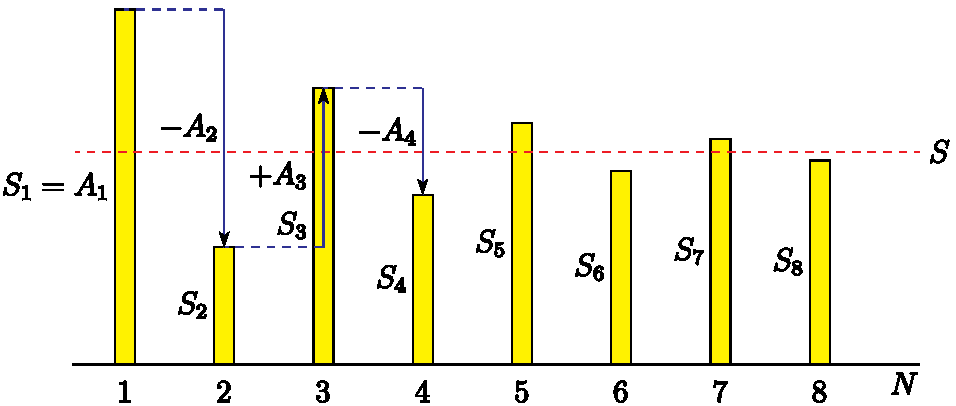
\includegraphics{altSeriesF.pdf}
\end{center}
\end{efig}
Here is a convergence test for alternating series that exploits
this structure, and that is really easy to apply.



\begin{theorem}[Alternating Series Test]\label{thm:SRalternating}
 Let $\big\{A_n\big\}_{n=1}^\infty$
be a sequence of real numbers that obeys
\begin{enumerate}[(i)]\itemsep1pt \parskip0pt \parsep0pt %\itemindent-15pt
\item $A_n\ge 0$ for all $n\ge 1$ and
\item $A_{n+1}\le A_n$  for all $n\ge 1$ (i.e. the
sequence is monotone decreasing) and
\item $\lim_{n\rightarrow\infty}A_n=0$.
\end{enumerate}
Then
\begin{equation*}
A_1-A_2+A_3-A_4+\cdots=\sum\limits_{n=1}^\infty (-1)^{n-1} A_n =S
\end{equation*}
converges and, for each natural number $N$,  $S-S_N$ is between $0$ and (the
first dropped term) $(-1)^N A_{N+1}$. Here $S_N$ is, as previously,
the $N^{\rm th}$ partial sum $\sum\limits_{n=1}^N (-1)^{n-1} A_n$.
\end{theorem}
\begin{proof}[``Proof''] We shall only give part of the proof here.
For the rest of the proof see the optional section \ref{sec:CompProof}.
We shall fix any natural number $N$ and concentrate on the last statement,
which gives a bound on the truncation error (which is the error introduced
when you approximate the full series by the partial sum $S_N$)
\begin{equation*}
E_N = S-S_N= \sum_{n=N+1}^\infty (-1)^{n-1} A_n
= (-1)^N\Big[A_{N+1}-A_{N+2} +A_{N+3}-A_{N+4}+\cdots\Big]
\end{equation*}
This is of course another series. We're going to study the partial sums
\begin{equation*}
S_{N,\ell} = \sum_{n=N+1}^\ell (-1)^{n-1} A_n
= (-1)^N\sum_{m=1}^{\ell-N} (-1)^{m-1} A_{N+m}
\end{equation*}
for that series.
\begin{itemize}
\item
If $\ell'>N+1$, with $\ell'-N$ even,
\begin{align*}
(-1)^N S_{N,\ell'}&=\overbrace{(A_{N+1}-A_{N+2})}^{\ge 0}
                +\overbrace{(A_{N+3}-A_{N+4})}^{\ge 0}+\cdots
                +\overbrace{(A_{\ell'-1}-A_{\ell'})}^{\ge 0}
                \ge 0\quad\hbox{and}\quad\\
(-1)^N S_{N,\ell'+1}&=\overbrace{(-1)^N S_{N,\ell'}}^{\ge 0}
                        +\overbrace{A_{\ell'+1}}^{\ge 0}
                   \ge 0
\end{align*}
This tells us that $(-1)^N S_{N,\ell}\ge 0$ for all $\ell>N+1$, both even and odd.
\item
Similarly, if $\ell'>N+1$, with $\ell'-N$ odd,
\begin{align*}
(-1)^N S_{N,\ell'}&=A_{N+1}-(\overbrace{A_{N+2}-A_{N+3}}^{\ge 0})
                         -(\overbrace{A_{N+4}-A_{N+5}}^{\ge 0})-\cdots
                         -\overbrace{(A_{\ell'-1}-A_{\ell'})}^{\ge 0}
            \le A_{N+1} \\
(-1)^NS_{N,\ell'+1}&=\overbrace{(-1)^N S_{N,\ell'}}^{\le A_{N+1}}
                          -\overbrace{A_{\ell'+1}}^{\ge 0}
               \le A_{N+1}
\end{align*}
This tells us that $(-1)^N S_{N,\ell}\le A_{N+1}$ for all  for all $\ell>N+1$,
both even and odd.
\end{itemize}
So we now know that $S_{N,\ell}$ lies between its first term, $(-1)^NA_{N+1}$,
and $0$ for all $\ell>N+1$. While we are not going to prove it here
(see the optional section \ref{sec:CompProof}), this implies
that, since $A_{N+1}\rightarrow 0$ as $N\rightarrow\infty$, the series
converges and that
\begin{equation*}
S-S_N=\lim_{\ell\rightarrow\infty} S_{N,\ell}
\end{equation*}
lies between $(-1)^NA_{N+1}$ and $0$.

\end{proof}

\begin{eg}\label{eg:SRaltharmonic}
We have already seen, in Example \ref{eg:SRpTest}, that the harmonic
series $\sum_{n=1}^\infty\frac{1}{n}$ diverges. On the other hand, the
series $\sum_{n=1}^\infty(-1)^{n-1}\frac{1}{n}$ converges by the alternating
series test with $A_n=\frac{1}{n}$. Note that
\begin{enumerate}[(i)]\itemsep1pt \parskip0pt \parsep0pt %\itemindent-15pt
\item $A_n=\frac{1}{n}\ge 0$ for all $n\ge 1$, so that
$\sum_{n=1}^\infty(-1)^{n-1}\frac{1}{n}$ really is an alternating series,
and
\item $A_n=\frac{1}{n}$ decreases as $n$ increases,  and
\item $\lim\limits_{n\rightarrow\infty}A_n
   =\lim\limits_{n\rightarrow\infty}\frac{1}{n}=0$.
\end{enumerate}
so that all of the hypotheses of the alternating series test,
i.e. of Theorem \ref{thm:SRalternating}, are satisfied. We shall see,
in Example~\ref{eg:SRpsrepC}, that
\begin{align*}
\sum_{n=1}^\infty \frac{(-1)^{n-1}}{n} &= \log 2.
\end{align*}
\end{eg}

\begin{eg}[$e$]\label{eg:SRaltharmonicB}
You may already know that
$
e^x=\sum_{n=0}^\infty\frac{x^n}{n!}
$. In any event, we shall prove this in Example~\ref{eg:expSeries},
below. In particular
\begin{align*}
\frac{1}{e}=e^{-1} = \sum_{n=0}^\infty\frac{(-1)^n}{n!}
 = 1 -\frac{1}{1!} +\frac{1}{2!} -\frac{1}{3!} +\frac{1}{4!}
                     - \frac{1}{5!}+\cdots
\end{align*}
is an alternating series and satisfies all of the conditions
of the alternating series test, Theorem~\ref{thm:SRalternating}a:
\begin{enumerate}[(i)]\itemsep1pt \parskip0pt \parsep0pt %\itemindent-15pt
\item The terms in the series alternate in sign.
\item The magnitude of the $n^{\rm th}$ term in the series decreases
            monotonically as $n$ increases.
\item The $n^{\rm th}$ term in the series converges to zero as
$n\rightarrow\infty$.
\end{enumerate}
So the alternating series test guarantees that, if we approximate,
for example,
\begin{align*}
\frac{1}{e} \approx \frac{1}{2!}-\frac{1}{3!} +\frac{1}{4!}-\frac{1}{5!}+\frac{1}{6!}-\frac{1}{7!}
+\frac{1}{8!}-\frac{1}{9!}
\end{align*}
then the error in this approximation lies between $0$ and the
next term in the series, which is $\frac{1}{10!}$. That is
\begin{align*}
\frac{1}{2!}-\frac{1}{3!} +\frac{1}{4!}-\frac{1}{5!}+\frac{1}{6!}-\frac{1}{7!}
+\frac{1}{8!}-\frac{1}{9!}
\le \frac{1}{e} \le
\frac{1}{2!}-\frac{1}{3!} +\frac{1}{4!}-\frac{1}{5!}+\frac{1}{6!}-\frac{1}{7!}
+\frac{1}{8!}-\frac{1}{9!}+\frac{1}{10!}
\end{align*}
so that
\begin{align*}
\frac{1}{
\frac{1}{2!}-\frac{1}{3!} +\frac{1}{4!}-\frac{1}{5!}+\frac{1}{6!}-\frac{1}{7!}
+\frac{1}{8!}-\frac{1}{9!}+\frac{1}{10!}}
\le e \le
\frac{1}{
\frac{1}{2!}-\frac{1}{3!} +\frac{1}{4!}-\frac{1}{5!}+\frac{1}{6!}-\frac{1}{7!}
+\frac{1}{8!}-\frac{1}{9!}}
\end{align*}
which, to seven decimal places says
\begin{align*}
2.7182816 \le e\le  &2.7182837
%2.718281657666403 \le e\le  &2.7182836938934494
\end{align*}
(To seven decimal places $e=2.7182818$.)
%$e=2.718281828459045$

The alternating series test tells us that, for any natural number $N$,
the error that we make when we approximate $\frac{1}{e}$ by the
partial sum $S_N= \sum_{n=0}^N\frac{(-1)^n}{n!}$ has magnitude no
larger than $\frac{1}{(N+1)!}$. This tends to zero spectacularly quickly
as $N$ increases, simply because $(N+1)!$ increases spectacularly quickly as $N$ increases\footnote{The interested reader may wish to check out
``Stirling's approximation'', which says that $n!\approx \sqrt {2\pi n}
\left(\frac {n}{e}\right)^{n}$.}. For example $20!\approx 2.4\times 10^{27}$.
\end{eg}

\begin{eg}\label{eg:SRaltLog}
We will shortly see, in Example \ref{eg:SRpsrepC},
that if $-1<x\le 1$, then
\begin{equation*}
\log(1+x) = x-\frac{x^2}{2}+\frac{x^3}{3}-\frac{x^4}{4}+\cdots
= \sum_{n=1}^\infty (-1)^{n-1}\frac{x^n}{n}
\end{equation*}
Suppose that we have to compute $\log\frac{11}{10}$ to within an
accuracy of $10^{-12}$. Since $\frac{11}{10}=1+\frac{1}{10}$,
we can get $\log\frac{11}{10}$ by evaluating $\log(1+x)$
at $x=\frac{1}{10}$, so that
\begin{equation*}
\log\frac{11}{10} = \log\Big(1+\frac{1}{10}\Big)
          =\frac{1}{10}
           -\frac{1}{2\times 10^2}
           +\frac{1}{3\times 10^3}
           -\frac{1}{4\times 10^4}+\cdots
= \sum_{n=1}^\infty (-1)^{n-1}\frac{1}{n\times 10^n}
\end{equation*}
By the alternating series test, this series converges. Also by the
alternating series test, approximating $\log\frac{11}{10}$ by
throwing away all but the first $N$ terms
\begin{equation*}
\log\frac{11}{10} \approx
          \frac{1}{10}
           -\frac{1}{2\times 10^2}
           +\frac{1}{3\times 10^3}
           -\frac{1}{4\times 10^4}+\cdots
           +(-1)^{N-1}\frac{1}{N\times 10^N}
= \sum_{n=1}^{N} (-1)^{n-1}\frac{1}{n\times 10^n}
\end{equation*}
introduces an error whose magnitude is no more than the magnitude
of the first term that we threw away.
\begin{equation*}
\text{error} \le \frac{1}{(N+1)\times 10^{N+1}}
\end{equation*}
To achieve an error that is no more than $10^{-12}$, we have to choose $N$ so
that
\begin{equation*}
\frac{1}{(N+1)\times 10^{N+1}} \le 10^{-12}
\end{equation*}
The best way to do so is simply to guess --- we are not going to be able
to manipulate the inequality
   $\frac{1}{(N+1)\times 10^{N+1}} \le \frac{1}{10^{12}}$
into the form $N\le \cdots$, and even if we could, it would not
be worth the effort.
We need to choose $N$ so that the denominator $(N+1)\times 10^{N+1}$
is at least $10^{12}$. That is easy, because the denominator contains the factor $10^{N+1}$ which is at least $10^{12}$ whenever $N+1\ge 12$, i.e.
whenever $N\ge 11$. So we will achieve an error of less than $10^{-12}$
if we choose $N=11$.
\begin{equation*}
\frac{1}{(N+1)\times 10^{N+1}}\bigg|_{N=11}
   = \frac{1}{12\times 10^{12}}
   < \frac{1}{10^{12}}
\end{equation*}
This is not the smallest possible choice of $N$, but in practice that
just doesn't matter --- your computer is not going to care whether or not you
ask it to compute a few extra terms. If you really need the smallest $N$
that obeys  $\frac{1}{(N+1)\times 10^{N+1}} \le \frac{1}{10^{12}}$,
you can next just try $N=10$, then $N=9$, and so on.
\begin{alignat*}{3}
\frac{1}{(N+1)\times 10^{N+1}}\bigg|_{N=11}
   &= \frac{1}{12\times 10^{12}}
   < \frac{1}{10^{12}} \\
\frac{1}{(N+1)\times 10^{N+1}}\bigg|_{N=10}
   &= \frac{1}{11\times 10^{11}}
   < \frac{1}{10\times 10^{11}} = \frac{1}{10^{12}} \\
\frac{1}{(N+1)\times 10^{N+1}}\bigg|_{N=9}
   &= \frac{1}{10\times 10^{10}}
   = \frac{1}{10^{11}}
   > \frac{1}{10^{12}}
\end{alignat*}
So in this problem, the smallest acceptable $N=10$.

\end{eg}


%%%%%%%%%%%%%%%%%%%%%%%%%%%%%
\subsection{The Ratio Test}\label{sec:RatioTest}
%%%%%%%%%%%%%%%%%%%%%%%%%%%%%
The idea behind the ratio test comes from a reexamination of the
geometric series. Recall that the geometric series
\begin{align*}
  \sum_{n=0}^\infty a_n = \sum_{n=0}^\infty a r^n
\end{align*}
converges when $|r|<1$ and diverges otherwise. So the convergence of
this series is completely determined by the number $r$. This number
is just the ratio of successive terms --- that is $r = a_{n+1}/a_n$.

In general the ratio of successive terms of a series,
$\frac{a_{n+1}}{a_n}$, is not constant, but depends on
$n$. However, as we have noted above, the convergence of a
series $\sum a_n$ is determined by the behaviour of its
terms when $n$ is large. In this way, the behaviour of this
ratio when $n$ is small tells us nothing about the
convergence of the series, but the limit of the ratio as $n\to\infty$
does. This is the basis of the ratio test.

\begin{theorem}[Ratio Test]\label{thm:SRratio}
Let $N$ be any positive integer and assume that $a_n\ne 0$ for all $n\ge N$.
\begin{enumerate}[(a)]
\item If $\lim\limits_{n\rightarrow\infty}\Big|\frac{a_{n+1}}{a_n}\Big| = L<1$,
then $\sum\limits_{n=1}^\infty a_n$ converges.
\item If $\lim\limits_{n\rightarrow\infty}\Big|\frac{a_{n+1}}{a_n}\Big| = L>1$,
or $\lim\limits_{n\rightarrow\infty}\Big|\frac{a_{n+1}}{a_n}\Big| = +\infty$,
then $\sum\limits_{n=1}^\infty a_n$ diverges.
\end{enumerate}
\end{theorem}

\begin{warning}
Beware that the ratio test provides absolutely no conclusion about the
convergence or divergence of the series $\sum\limits_{n=1}^\infty a_n$
if $\lim\limits_{n\rightarrow\infty}\Big|\frac{a_{n+1}}{a_n}\Big| =  1$.
See Example \ref{eg:SRratioC}, below.
\end{warning}

\begin{proof}
(a) Pick any number $R$ obeying $L<R<1$. We are assuming that
$\Big|\frac{a_{n+1}}{a_n}\Big|$ approaches $L$ as $n\rightarrow\infty$.
In particular there must be some natural number $M$ so that
$\Big|\frac{a_{n+1}}{a_n}\Big|\le R$ for all $n\ge M$. So
$|a_{n+1}|\le R|a_n|$ for all $n\ge M$. In particular
\begin{alignat*}{3}
|a_{M+1}| & \ \le\  R\,|a_M| \\
|a_{M+2}| & \ \le\  R\,|a_{M+1}| &\ \ \le\  R^2 \,|a_M| \\
|a_{M+3}| & \ \le\  R\,|a_{M+2}| &\ \ \le\  R^3 \,|a_M| \\
&\vdots \\
|a_{M+\ell}| &\le R^\ell \,|a_M|
\end{alignat*}
for all $\ell\ge 0$. The series $\sum_{\ell=0}^\infty  R^\ell \,|a_M|$
is a geometric series with ratio $R$ smaller than one in magnitude and
so converges. Consequently, by the comparison test with $a_n$ replaced
by $A_\ell = a_{n+\ell}$ and $c_n$ replaced by $C_\ell= R^\ell \, |a_M|$,
the series $\sum\limits_{\ell=1}^\infty a_{M+\ell}
=\sum\limits_{n=M+1}^\infty a_n$ converges. So the series
$\sum\limits_{n=1}^\infty a_n$ converges too.

\noindent (b) We are assuming that
$\Big|\frac{a_{n+1}}{a_n}\Big|$ approaches $L>1$ as $n\rightarrow\infty$.
In particular there must be some natural number $M>N$ so that
$\Big|\frac{a_{n+1}}{a_n}\Big|\ge 1$ for all $n\ge M$. So
$|a_{n+1}|\ge |a_n|$ for all $n\ge M$. That is, $|a_n|$ increases as $n$
increases as long as $n\ge M$. So $|a_n|\ge |a_M|$ for all $n\ge M$
and $a_n$ cannot converge to zero as $n\rightarrow\infty$. So the series
diverges by the divergence test.

\end{proof}


\begin{eg}[$\sum_{n=0}^\infty a n x^{n-1}$]\label{eg:SRratioA}
Fix any two nonzero real numbers $a$ and $x$. We have already seen
in Example \ref{eg:SRgeom} --- we have just renamed $r$ to $x$ ---
that the geometric series $\sum_{n=0}^\infty a x^n$ converges when $|x|<1$
and diverges when $|x|\ge 1$. We are now going to consider a new series,
constructed by differentiating\footnote{We shall see later, in
Theorem \ref{thm:SRpsops}, that the function
$\sum_{n=0}^\infty a n x^{n-1}$ is indeed the derivative of the
function $\sum_{n=0}^\infty a x^n$. Of course, such a statement
only makes sense where these series converge --- how can you differentiate
a divergent series? (This is not an allusion to a popular series of dystopian novels.) Actually, there is quite a bit of interesting and useful
mathematics involving divergent series, but it is well beyond the scope
of this course.} each term in the geometric series
$\sum_{n=0}^\infty a x^n$. This new series is
\begin{equation*}
\sum_{n=0}^\infty a_n\qquad\text{with}\quad a_n = a\, n\, x^{n-1}
\end{equation*}
Let's apply the ratio test.
\begin{align*}
\Big|\frac{a_{n+1}}{a_n}\Big|
&= \Big|\frac{a\, (n+1)\, x^n}{a\, n\, x^{n-1}}\Big|
 = \frac{n+1}{n} |x|
 = \Big(1+\frac{1}{n}\Big) |x|
\rightarrow L=|x|\quad\text{as $n\rightarrow\infty$}
\end{align*}
The ratio test now tells us that the series $\sum_{n=0}^\infty a\, n\, x^{n-1}$
converges if $|x|<1$ and diverges if $|x|>1$. It says nothing
about the cases $x=\pm 1$. But in both of those cases $a_n=a\,n\,(\pm 1)^n$
does not converge to zero as $n\rightarrow\infty$ and the series
diverges by the divergence test.
\intremark{
The ``popular series of dystopian novels'' refers to
``The Divergent trilogy is a series of young adult science fiction adventure novels by American novelist Veronica Roth set in a post-apocalyptic dystopian Chicago''.
}
\end{eg}

Notice that in the above example, we had to apply another convergence
test in addition to the ratio test. This will be commonplace when we
reach power series and Taylor series --- the ratio test will tell us
something like
\begin{quote}
 The series converges for $|x|<R$ and diverges for $|x|>R$.
\end{quote}
Of course, we will still have to to determine what happens when $x=+R, -R$. To determine convergence or divergence in those cases we  will
need to use one of the other tests we have seen.

\begin{eg}[$\sum_{n=0}^\infty \frac{a}{n+1} X^{n + 1}$]\label{eg:SRratioB}
Once again, fix any two nonzero real numbers $a$ and $X$.
We again start with the geometric series $\sum_{n=0}^\infty a x^n$
but this time we construct a new series by integrating\footnote{We shall
also see later, in Theorem \ref{thm:SRpsops}, that the function
$\sum_{n=0}^\infty \frac{a}{n+1} x^{n + 1}$ is indeed an antiderivative
of the function $\sum_{n=0}^\infty a x^n$.} each term,
$a x^n$, from $x=0$ to $x=X$ giving $\frac{a}{n+1} X^{n + 1}$. The resulting
new series is
\begin{equation*}
\sum_{n=0}^\infty a_n\qquad\text{with }a_n = \frac{a}{n+1} X^{n + 1}
\end{equation*}
To apply the ratio test we need to compute
\begin{align*}
\Big|\frac{a_{n+1}}{a_n}\Big|
&= \bigg|\frac{\frac{a}{n+2} X^{n + 2}}{\frac{a}{n+1} X^{n + 1}}\bigg|
 = \frac{n+1}{n+2} |X|
 = \frac{1+\frac{1}{n}}{1+\frac{2}{n}} |X|
\rightarrow L=|X|\quad\text{as $n\rightarrow\infty$}
\end{align*}
The ratio test now tells us that the series
$\sum_{n=0}^\infty \frac{a}{n+1} X^{n + 1}$
converges if $|X|<1$ and diverges if $|X|>1$. It says nothing
about the cases $X=\pm 1$.

 If $X=1$, the series reduces to
\begin{equation*}
\sum_{n=0}^\infty \frac{a}{n+1} X^{n + 1}\bigg|_{X=1}
=\sum_{n=0}^\infty \frac{a}{n+1}
=a\sum_{m=1}^\infty \frac{1}{m}\qquad\text{with }m=n+1
\end{equation*}
which is just $a$ times the harmonic series, which we know diverges,
by Example \ref{eg:SRpTest}.

If $X=-1$, the series reduces to
\begin{equation*}
\sum_{n=0}^\infty \frac{a}{n+1} X^{n + 1}\bigg|_{X=-1}
=\sum_{n=0}^\infty (-1)^{n+1}\frac{a}{n+1}
\end{equation*}
which converges by the alternating series test.
See Example \ref{eg:SRaltharmonic}.

In conclusion, the series $\sum_{n=0}^\infty \frac{a}{n+1} X^{n + 1}$
converges if and only if $-1\le X<1$.
\end{eg}

The ratio test is often quite easy to apply, but one must always be
careful when the limit of the ratio is $1$. The next example
illustrates this.


\begin{eg}[$L=1$]\label{eg:SRratioC}
In this example, we are going to see three different series that all have
$\lim_{n\rightarrow\infty}\Big|\frac{a_{n+1}}{a_n}\Big| = 1$. One
is going to diverge and the other two are going to converge.

\begin{itemize}
\item
The first series is the harmonic series
\begin{equation*}
\sum_{n=1}^\infty a_n\qquad\text{with }a_n = \frac{1}{n}
\end{equation*}
We have already seen, in Example \ref{eg:SRpTest}, that this series diverges.
It has
\begin{equation*}
\Big|\frac{a_{n+1}}{a_n}\Big|
= \bigg|\frac{\frac{1}{n+1}}{\frac{1}{n}}\bigg|
 = \frac{n}{n+1}
 = \frac{1}{1+\frac{1}{n}}
\rightarrow L=1\quad\text{as $n\rightarrow\infty$}
\end{equation*}

\item
The second series is the alternating harmonic series
\begin{equation*}
\sum_{n=1}^\infty a_n\qquad\text{with }a_n = (-1)^{n-1}\frac{1}{n}
\end{equation*}
We have already seen, in Example \ref{eg:SRaltharmonic}, that this series converges.
But it also has
\begin{equation*}
\Big|\frac{a_{n+1}}{a_n}\Big|
= \bigg|\frac{(-1)^n\frac{1}{n+1}}{(-1)^{n-1}\frac{1}{n}}\bigg|
 = \frac{n}{n+1}
 = \frac{1}{1+\frac{1}{n}}
\rightarrow L=1\quad\text{as $n\rightarrow\infty$}
\end{equation*}

\item
The third series is
\begin{equation*}
\sum_{n=1}^\infty a_n\qquad\text{with }a_n = \frac{1}{n^2}
\end{equation*}
We have already seen, in Example \ref{eg:SRpTest} with $p=2$,
that this series converges. But it also has
\begin{equation*}
\Big|\frac{a_{n+1}}{a_n}\Big|
= \bigg|\frac{\frac{1}{(n+1)^2}}{\frac{1}{n^2}}\bigg|
 = \frac{n^2}{(n+1)^2}
 = \frac{1}{(1+\frac{1}{n})^2}
\rightarrow L=1\quad\text{as $n\rightarrow\infty$}
\end{equation*}

\end{itemize}
\end{eg}

Let's do a somewhat artificial example that forces us to combine a few of the techniques we have seen.
\begin{eg}[$\sum_{n=1}^\infty \frac{ (-3)^n \sqrt{n+1}}{2n+3}x^n$]
   \label{eg:ratioC}
 Again, the convergence of this series will depend on $x$.
 \begin{itemize}
  \item Let us start with the ratio test --- so we compute
 \begin{align*}
  \left|\frac{a_{n+1}}{a_n}\right|
  &= \left|\frac{(-3)^{n+1} \sqrt{n+2} (2n+3) x^{n+1} }{(-3)^n \sqrt{n+1} (2n+5) x^n} \right|\\
  &= |-3| \cdot \frac{\sqrt{n+2}}{\sqrt{n+1}} \cdot \frac{2n+3}{2n+5} \cdot |x|
  \intertext{So in the limit as $n \to \infty$ we are left with}
  \lim_{n\to\infty} \left|\frac{a_{n+1}}{a_n}\right|
  &= 3 |x|
\end{align*}
\item The ratio test then tells us that if $3|x|>1$ the series diverges, while when $3|x|<1$ the series converges.
\item This leaves us with the cases $x=+\frac{1}{3}$ and $-\frac{1}{3}$.
\item Setting $x=\frac{1}{3}$ gives the series
\begin{align*}
\sum_{n=1}^\infty \frac{ (-1)^n \sqrt{n+1}}{2n+3}
\end{align*}
The fact that the terms alternate here suggests that we use the alternating series test. That will show that this
series converges provided $\frac{\sqrt{n+1}}{2n+3}$ decreases as $n$ increases.
So we define the function
\begin{align*}
  f(t) &= \frac{\sqrt{t+1}}{2t+3}
\end{align*}
(which is constructed by replacing the $n$ in $\frac{\sqrt{n+1}}{2n+3}$ with $t$)
and verify that $f(t)$ is a decreasing function of $t$. To prove that, it suffices to show its derivative is negative when $t\geq 1$:
\begin{align*}
  f'(t) &= \frac{(2t+3)\cdot \frac{1}{2} \cdot(t+1)^{-1/2} - 2\sqrt{t+1} }{(2t+3)^2}\\
  &=\frac{(2t+3) - 4(t+1)  }{2 \sqrt{t+1} (2t+3)^2}\\
  &= \frac{-2t-1}{2 \sqrt{t+1} (2t+3)^2}
\end{align*}
When $t \geq 1$ this is negative and so $f(t)$ is a decreasing function. Thus we can apply the alternating series
test to show that the series converges when $x=\frac{1}{3}$.

\item When $x = -\frac{1}{3}$ the series becomes
\begin{align*}
\sum_{n=1}^\infty \frac{\sqrt{n+1}}{2n+3}.
\end{align*}
Notice that when $n$ is large, the summand is approximately
$\frac{\sqrt{n}}{2n}$ which suggests that the series will diverge
by comparison with $\sum n^{-1/2}$. To formalise this, we can use the limit comparison theorem:
\begin{align*}
  \lim_{n \to \infty} \frac{\sqrt{n+1}}{2n+3}\  \frac{1}{ n^{-1/2} }
  &=
  \lim_{n \to \infty} \frac{\sqrt{n} \cdot \sqrt{1+1/n}}{n(2+3/n)} \cdot n^{1/2}\\
  &=
  \lim_{n \to \infty} \frac{n \cdot \sqrt{1+1/n}}{n(2+3/n)} \\
  &= \frac{1}{2}
\end{align*}
So since this ratio has a finite limit and the series $\sum n^{-1/2}$ diverges, we know that our series also diverges.
\end{itemize}
So in summary the series converges when $-\frac{1}{3} < x \leq \frac{1}{3}$ and diverges otherwise.
\end{eg}

%%%%%%%%%%%%%%%%%%%%%%%%%%%%%
\subsection{Convergence Test List}
%%%%%%%%%%%%%%%%%%%%%%%%%%%%%
We now have half a dozen convergence tests:
\begin{itemize}
\item
\emph{Divergence Test}
\begin{itemize}
\item
works well when the $n^{\mathrm{th}}$ term in the series \emph{fails}
to converge to zero as $n$ tends to infinity
\end{itemize}
%%%
\item
\emph{Alternating Series Test}
\begin{itemize}
\item
works well when successive terms in the series alternate
in sign
\item
don't forget to check that successive terms decrease in magnitude
and tend to zero as $n$  tends to infinity
\end{itemize}
%%%
\item
\emph{Integral Test}
\begin{itemize}
\item
works well when, if you substitute $x$ for $n$ in the $n^{\mathrm{th}}$ term
you get a function, $f(x)$, that you can integrate
\item
don't forget to check that $f(x)\ge 0$ and that $f(x)$ decreases
as $x$ increases
\end{itemize}

%%%
\item
\emph{Ratio Test}
\begin{itemize}
\item
works well when $\frac{a_{n+1}}{a_n}$ simplifies enough that
you can easily compute
$\lim\limits_{n\rightarrow\infty}\big|\frac{a_{n+1}}{a_n}\big|=L$
\item
this often happens when $a_n$ contains powers, like $7^n$,
or factorials, like $n!$
\item
don't forget that $L=1$ tells you nothing about the convergence/divergence
of the series
\end{itemize}

%%%
\item
\emph{Comparison Test and Limit Comparison Test}
\begin{itemize}
\item
works well when, for very large $n$, the $n^{\mathrm{th}}$ term
$a_n$ is approximately the same as a simpler term $b_n$ (see Example
\ref{eg:SRcomparisonTestB}) and it is easy to determine whether
or not $\sum_{n=1}^\infty b_n$ converges
\item
don't forget to check that $b_n\ge 0$
\item usually the Limit Comparison Test is easier to apply
than the Comparison Test
\end{itemize}

\end{itemize}

%%%%%%%%%%%%%%%%%%%
\subsection{Optional --- The Leaning Tower of Books}\label{sec:Stack}
%%%%%%%%%%%%%%%%%%%
Imagine that you are about to stack a bunch of identical books on a
table. But you don't want to just stack them exactly vertically.
You want to built a ``leaning tower of books'' that overhangs the
edge of the table as much as possible.
\begin{efig}
\begin{center}
     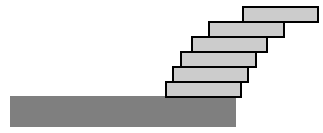
\includegraphics{bookStack.pdf}
\end{center}
\end{efig}
How big an overhang can you get? The answer to that question, which we'll now
derive, uses a series!
\begin{itemize}
\item
Let's start by just putting book \#1 on the table. It's the red book
labelled ``$B_1$'' in the figure below.
\begin{efig}
\begin{center}
     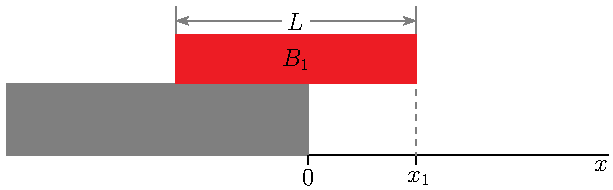
\includegraphics{bookStackV1.pdf}
\end{center}
\end{efig}
Use a horizontal $x$--axis with $x=0$ corresponding to the right hand
edge of the table. Imagine that we have placed book \#1 so that its
right hand edge overhangs the end of the table by a distance $x_1$.
\begin{itemize}\itemsep1pt \parskip0pt \parsep0pt \itemindent-10pt
\item[$\circ$]
In order for the book to not topple off of the table, we need its
centre of mass to lie above the table. That is, we need the $x$--coordinate
of the centre mass of $B_1$, which we shall denote $\bar X(B_1)$, to obey
\begin{equation*}
\bar X(B_1) \le 0
\end{equation*}
Assuming that our books have uniform density and are of length
$L$, $\bar X(B_1)$ will be exactly half way between the right hand end of the
book, which is at $x=x_1$, and the left hand end of the book, which is at
$x=x_1-L$. So
\begin{equation*}
\bar X(B_1) =\frac{1}{2} x_1+\frac{1}{2}(x_1-L)
            = x_1-\frac{L}{2}
\end{equation*}
\end{itemize}
Thus book \#1 does not topple off of the table provided
\begin{equation*}
x_1\le\frac{L}{2}
\end{equation*}

\item
Now let's put books \#1 and \#2 on the table, with the right hand edge of
book \#$1$ at $x=x_1$ and the right hand edge of book \#2 at
$x=x_2$, as in the figure below.
\begin{efig}
\begin{center}
     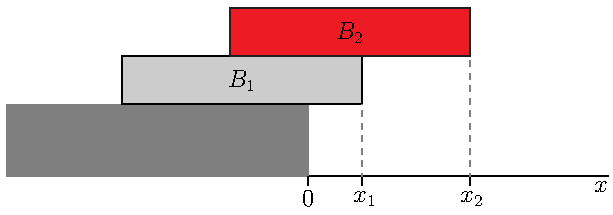
\includegraphics{bookStackV2a.pdf}
\end{center}
\end{efig}

\begin{itemize}\itemsep1pt \parskip0pt \parsep0pt \itemindent-10pt
\item[$\circ$]
In order for book \#2 to not topple off of book \#1, we need the
centre of mass of book \#2 to lie above book \#1. That is, we need
the $x$--coordinate of the centre mass of $B_2$, which is
$\bar X(B_2)=x_2-\frac{L}{2}$, to obey
\begin{equation*}
\bar X(B_2) \le x_1
\iff
x_2-\frac{L}{2} \le x_1
\iff
x_2\le x_1+\frac{L}{2}
\end{equation*}
\item[$\circ$]
Assuming that book \#2 does not topple off of book \#1, we still
need to arrange that the pair of books does not topple off of the table.
Think of the pair of books as the combined red object in the figure
\begin{efig}
\begin{center}
     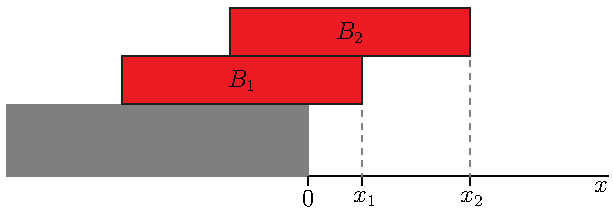
\includegraphics{bookStackV2b.pdf}
\end{center}
\end{efig}
In order for the combined red object to not topple off of the table,
we need the centre of mass of the combined red object to lie above
the table. That is, we need the $x$--coordinate
of the centre mass of the combined red object, which we shall denote
$\bar X(B_1\cup B_2)$, to obey
\begin{equation*}
\bar X(B_1\cup B_2) \le 0
\end{equation*}
The centre of mass of the combined red object is the weighted
average\footnote{It might be a good idea to review the beginning of
\S\ref{sec com} at this point.} of the centres of mass of $B_1$ and $B_2$.
As $B_1$ and $B_2$ have the same weight,
\begin{align*}
\bar X(B_1\cup B_2) &= \frac{1}{2}\bar X(B_1) +\frac{1}{2}\bar X(B_2)
    = \frac{1}{2}\Big(x_1-\frac{L}{2}\Big) +\frac{1}{2}\Big(x_2-\frac{L}{2}\Big)
\\
&= \frac{1}{2}(x_1+x_2) -\frac{L}{2}
\end{align*}
and the combined red object does not topple off of the table if
\begin{equation*}
\bar X(B_1\cup B_2)
=\frac{1}{2}(x_1+x_2) -\frac{L}{2} \le 0
\iff
x_1+x_2\le L
\end{equation*}
\end{itemize}
In conclusion, our two--book tower survives if
%\begin{align*}
%x_2\le x_1+\frac{L}{2}\qquad\text{and}\qquad x_1+x_2\le L
%\iff x_2\le\min\Big\{x_1+\frac{L}{2}, L-x_1\Big\}
%\end{align*}
%Here  $\min\Big\{x_1+\frac{L}{2}, L-x_1\Big\}$ means the minimum of
%$x_1+\frac{L}{2}$ and $L-x_1$.
\begin{align*}
x_2\le x_1+\frac{L}{2}\qquad\text{and}\qquad x_1+x_2\le L
\end{align*}
In particular we may choose $x_1$ and $x_2$ to satisfy
$x_2 = x_1+\frac{L}{2}$ and $x_1+x_2 = L$. Then, substituting
$x_2 = x_1+\frac{L}{2}$ into $x_1+x_2 = L$ gives
\begin{equation*}
x_1 + \Big(x_1+\frac{L}{2}\Big) = L
\iff 2x_1 = \frac{L}{2}
\iff x_1 = \frac{L}{2}\Big(\frac{1}{2}\Big),\quad
     x_2 = \frac{L}{2}\Big(1+\frac{1}{2}\Big)
\end{equation*}

\item
Before considering the general ``$n$--book tower'', let's now put
books \#1, \#2 and \#3
on the table, with the right hand edge of book \#1 at $x=x_1$,
the right hand edge of book \#2 at  $x=x_2$, and the right
hand edge of book \#3 at $x=x_3$, as in the figure below.
\begin{efig}
\begin{center}
     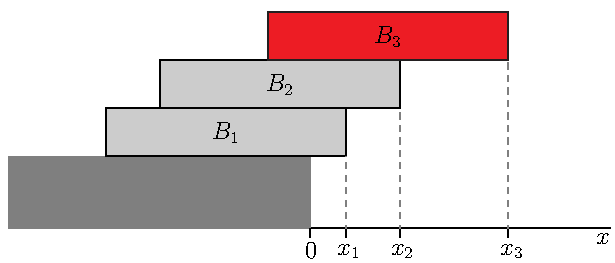
\includegraphics{bookStackV3a.pdf}
\end{center}
\end{efig}
\begin{itemize}\itemsep1pt \parskip0pt \parsep0pt \itemindent-10pt
\item[$\circ$]
In order for book \#3 to not topple off of book \#2, we need the
centre of mass of book \#3 to lie above book \#2. That is, we need
the $x$--coordinate of the centre mass of $B_3$, which is
$\bar X(B_3)=x_3-\frac{L}{2}$, to obey
\begin{equation*}
\bar X(B_3) \le x_2
\iff
x_3-\frac{L}{2} \le x_2
\iff
x_3\le x_2+\frac{L}{2}
\end{equation*}
\item[$\circ$]
Assuming that book \#3 does not topple off of book \#2, we still
need to arrange that the pair of books, book \#2 plus book \#3 (the
red object in the figure below), does not topple off of book \#1.
\begin{efig}
\begin{center}
     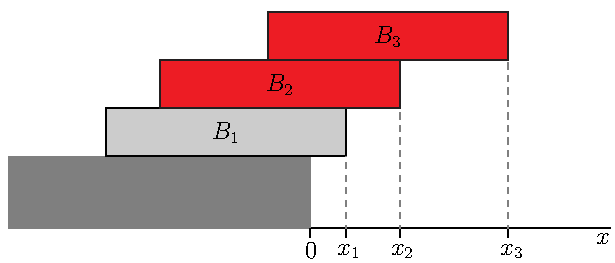
\includegraphics{bookStackV3b.pdf}
\end{center}
\end{efig}
In order for this combined red object to not topple off of book \#1,
we need the $x$--coordinate of its centre mass, which we denote
$\bar X(B_2\cup B_3)$, to obey
\begin{equation*}
\bar X(B_2\cup B_3) \le x_1
\end{equation*}
The centre of mass of the combined red object is the weighted
average  of the centre of masses of $B_2$ and $B_3$.
As $B_2$ and $B_3$ have the same weight,
\begin{align*}
\bar X(B_2\cup B_3) &= \frac{1}{2}\bar X(B_2) +\frac{1}{2}\bar X(B_3)
    = \frac{1}{2}\Big(x_2-\frac{L}{2}\Big)
      +\frac{1}{2}\Big(x_3-\frac{L}{2}\Big)
\\
&= \frac{1}{2}(x_2+x_3) -\frac{L}{2}
\end{align*}
and the combined red object does not topple off of book \#1 if
\begin{equation*}
\frac{1}{2}(x_2+x_3) -\frac{L}{2} \le x_1
\iff
x_2+x_3\le 2x_1+L
\end{equation*}

\item[$\circ$]
Assuming that book \#3 does not topple off of book \#2, and also
that the combined book \#2 plus book \#3 does not topple off of book \#1,
we still need to arrange that the whole tower of books, book \#1 plus
book \#2 plus book \#3 (the red object in the figure below), does not
topple off of the table.
\begin{efig}
\begin{center}
     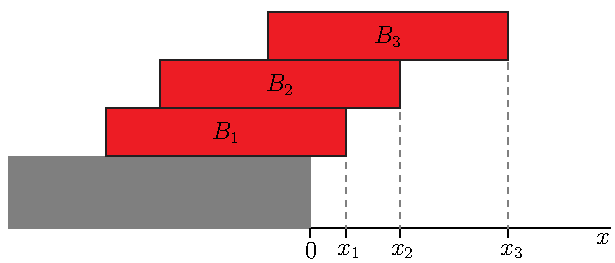
\includegraphics{bookStackV3c.pdf}
\end{center}
\end{efig}
In order for this combined red object to not topple off of the table,
we need the $x$--coordinate of its centre mass, which we denote
$\bar X(B_1\cup B_2\cup B_3)$, to obey
\begin{equation*}
\bar X(B_1\cup B_2\cup B_3) \le 0
\end{equation*}
The centre of mass of the combined red object is the weighted
average  of the centre of masses of $B_1$ and $B_2$ and $B_3$.
As they all have the same weight,
\begin{align*}
\bar X(B_1\cup B_2\cup B_3) &= \frac{1}{3}\bar X(B_1) +\frac{1}{3}\bar X(B_2)
                                +\frac{1}{3}\bar X(B_3) \\
  &=  \frac{1}{3}\Big(x_1-\frac{L}{2}\Big)
     +\frac{1}{3}\Big(x_2-\frac{L}{2}\Big)
     +\frac{1}{3}\Big(x_3-\frac{L}{2}\Big) \\
&= \frac{1}{3}(x_1+x_2+x_3) -\frac{L}{2}
\end{align*}
and the combined red object does not topple off of the table if
\begin{equation*}
\frac{1}{3}(x_1+ x_2+x_3) -\frac{L}{2} \le 0
\iff
x_1+ x_2+x_3\le \frac{3L}{2}
\end{equation*}
\end{itemize}
In conclusion, our three--book tower survives if
\begin{align*}
x_3\le x_2+\frac{L}{2}\qquad\text{and}\qquad x_2+x_3\le 2x_1 + L
\qquad\text{and}\qquad x_1+ x_2+x_3\le \frac{3L}{2}
\end{align*}
In particular, we may choose $x_1$, $x_2$ and $x_3$ to satisfy
\begin{align*}
x_1+ x_2+x_3&= \frac{3L}{2}\qquad\text{and} \\
x_2+x_3&= 2x_1 + L \qquad\text{and} \\
x_3 &= \frac{L}{2} + x_2
\end{align*}
Substituting the second equation into the first gives
\begin{align*}
3x_1 +L = \frac{3L}{2}
\implies x_1 = \frac{L}{2}\Big(\frac{1}{3}\Big)
\end{align*}
Next substituting the third equation into the second, and then
using the formula above for $x_1$, gives
\begin{align*}
2x_2 +\frac{L}{2} = 2x_1+L = \frac{L}{3} + L
\implies x_2 = \frac{L}{2}\Big(\frac{1}{2}+\frac{1}{3}\Big)
\end{align*}
and finally
\begin{align*}
     x_3 = \frac{L}{2} + x_2
         = \frac{L}{2}\Big(1+\frac{1}{2}+\frac{1}{3}\Big)
\end{align*}


\item
We are finally ready for the general ``$n$--book tower''.
Stack $n$ books on the table,
with book $B_1$ on the bottom and book $B_n$ at the top, and
with the right hand edge of book \#$j$ at $x=x_j$. The same
centre of mass considerations as above show that the tower survives
if
\begin{align*}
\bar X(B_n) &\le x_{n-1} &
x_n-\frac{L}{2}&\le x_{n-1} \\
%
\bar X(B_{n-1}\cup B_n) &\le x_{n-2} &
\frac{1}{2}(x_{n-1}+x_n)-\frac{L}{2}&\le x_{n-2} \\
%
&\ \ \vdots &\quad\vdots \\
%
\bar X(B_3\cup\cdots\cup B_n) &\le x_2&
\frac{1}{n-2}(x_3+\cdots+x_n)-\frac{L}{2}&\le x_2 \\
%
\bar X(B_2\cup B_3\cup\cdots\cup B_n) &\le x_1&
\frac{1}{n-1}(x_2+x_3+\cdots+x_n)-\frac{L}{2}&\le x_1 \\
%
\bar X(B_1\cup B_2\cup B_3\cup\cdots\cup B_n) &\le 0 &
\frac{1}{n}(x_1+x_2+x_3+\cdots+x_n)-\frac{L}{2}&\le 0
\end{align*}
In particular, we may choose the $x_j$'s to obey
\begin{align*}
\frac{1}{n}(x_1+x_2+x_3+\cdots+x_n)& = \frac{L}{2} \\
\frac{1}{n-1}(x_2+x_3+\cdots+x_n)&= \frac{L}{2} + x_1 \\
\frac{1}{n-2}(x_3+\cdots+x_n)&= \frac{L}{2}  + x_2 \\
&\ \ \vdots &\vdots& \\
\frac{1}{2}(x_{n-1}+x_n)&= \frac{L}{2} + x_{n-2} \\
x_n&= \frac{L}{2} + x_{n-1}
\end{align*}
Substituting $x_2+x_3+\cdots+x_n=(n-1) x_1  +\frac{L}{2}(n-1)$
from the second equation into the first
equation gives
\begin{align*}
\frac{1}{n}\Big\{\overbrace{x_1+(n-1) x_1}^{nx_1}
                  +\frac{L}{2}(n-1)\Big\} = \frac{L}{2}
&\implies x_1 +\frac{L}{2}\Big(1-\frac{1}{n}\Big)
           = \frac{L}{2}\Big(\frac{1}{2}\Big) \\
&\implies x_1 = \frac{L}{2}\Big(\frac{1}{n}\Big)
\end{align*}
Substituting $x_3+\cdots+x_n=(n-2) x_2+\frac{L}{2}(n-2)$ from the
third equation into the second
equation gives
\begin{align*}
&\frac{1}{n-1}\Big\{\overbrace{x_2+(n-2) x_2}^{(n-1)x_2}
      +\frac{L}{2}(\overbrace{n-2}^{(n-1)-1})\Big\} = \frac{L}{2} +x_1
=\frac{L}{2}\Big(1+\frac{1}{n}\Big) \\
&\hskip1in\implies x_2 + \frac{L}{2}\Big(1-\frac{1}{n-1}\Big)
    =\frac{L}{2}\Big(1+\frac{1}{n}\Big) \\
&\hskip1in\implies x_2 = \frac{L}{2}\Big(\frac{1}{n-1}+\frac{1}{n}\Big)
\end{align*}
Just keep going. We end up with
\begin{align*}
x_1 &= \frac{L}{2}\Big(\frac{1}{n}\Big)  \\
x_2 &= \frac{L}{2}\Big(\frac{1}{n-1}+\frac{1}{n}\Big) \\
x_3 &= \frac{L}{2}\Big(\frac{1}{n-2}+\frac{1}{n-1}+\frac{1}{n}\Big) \\
    &\ \  \vdots \\
x_{n-2} &= \frac{L}{2}\Big(\frac{1}{3}+\cdots+\frac{1}{n}\Big) \\
x_{n-1} &= \frac{L}{2}\Big(\frac{1}{2}+\frac{1}{3}+\cdots+\frac{1}{n}\Big) \\
x_n &= \frac{L}{2}\Big(1+\frac{1}{2}+\frac{1}{3}+\cdots+\frac{1}{n}\Big)
\end{align*}
Our overhang is $x_n = \frac{L}{2}\big(1+\frac{1}{2}+\frac{1}{3}+\cdots+\frac{1}{n}\big)$.
This is $\frac{L}{2}$ times the $n^{\rm th}$ partial sum of the
harmonic series $\sum_{m=1}^\infty\frac{1}{m}$. As we saw in Example
\ref{eg:SRpTest} (the $p$ test), the harmonic series diverges.
So, as $n$ goes to infinity $1+\frac{1}{2}+\frac{1}{3}+\cdots+\frac{1}{n}$
also goes to infinity.
We may make the overhang as large\footnote{At least if our table is strong enough.} as we like!

\end{itemize}

%%%%%%%%%%%%%%%%%%%
\subsection{Optional --- The Root Test}\label{sec:RootTest}
%%%%%%%%%%%%%%%%%%%

There is another test that is very similar in spirit to the
ratio test. It also comes from a reexamination of the
geometric series
\begin{align*}
  \sum_{n=0}^\infty a_n = \sum_{n=0}^\infty a r^n
\end{align*}
The ratio test was based on the observation that $r$, which largely
determines whether or not the series converges, could be found by
computing the ratio $r = a_{n+1}/a_n$. The root test is based on
the observation that $|r|$ can also be determined by looking that
the $n^{\rm th}$ root of the $n^{\rm th}$ term with $n$ very large:
\begin{equation*}
\lim_{n\to\infty}\root{n}\of{\big|ar^n\big|}
=|r|\lim_{n\to\infty}\root{n}\of{\big|a\big|}
=|r|\qquad\text{if $a\ne 0$}
\end{equation*}
Of course, in general, the $n^{\rm th}$ term is not exactly $ar^n$.
However, if for very large $n$, the $n^{\rm th}$ term is
approximately proportional to $r^n$, with $|r|$ given by the above limit,
we would expect the series to converge when $|r|<1$ and diverge when $|r|>1$.
That is indeed the case.

\begin{theorem}[Root Test]\label{thm:SRroot}
Assume that
\begin{equation*}
L = \lim_{n\to\infty}\root{n}\of{\big|a_n\big|}
\end{equation*}
exists or is $+\infty$.
\begin{enumerate}[(a)]
\item If $L<1$, then $\sum\limits_{n=1}^\infty a_n$ converges.
\item If $L>1$, or $L=+\infty$,
then $\sum\limits_{n=1}^\infty a_n$ diverges.
\end{enumerate}
\end{theorem}

\begin{warning}
Beware that the root test provides absolutely no conclusion about the
convergence or divergence of the series $\sum\limits_{n=1}^\infty a_n$
if $\lim\limits_{n\rightarrow\infty}\root{n}\of{\big|a_n\big|} =  1$.
\end{warning}

\begin{proof}
(a) Pick any number $R$ obeying $L<R<1$. We are assuming that
$\root{n}\of{|a_n|}$ approaches $L$ as $n\rightarrow\infty$.
In particular there must be some natural number $M$ so that
$\root{n}\of{|a_n|}\le R$ for all $n\ge M$. So
$|a_n|\le R^n$ for all $n\ge M$ and the series
$\sum\limits_{n=1}^\infty a_n$ converges by comparison to the geometric
series $\sum\limits_{n=1}^\infty R^n$

\noindent (b) We are assuming that
$\root{n}\of{|a_n|}$ approaches $L>1$ (or grows unboundedly)
as $n\rightarrow\infty$. In particular there must be some natural
number $M$ so that $\root{n}\of{|a_n|}\ge 1$ for all $n\ge M$.
So $|a_n|\ge 1$ for all $n\ge M$ and the series diverges by the
divergence test.

\end{proof}

\begin{eg}[$\sum_{n=1}^\infty \frac{ (-3)^n \sqrt{n+1}}{2n+3}x^n$]
\label{eg:rootA}
 We have already used the ratio test, in Example \ref{eg:ratioC},
to show that this series converges when $|x|<\frac{1}{3}$ and diverges
when $|x|>\frac{1}{3}$. We'll now use the root test to draw the
same conclusions.
 \begin{itemize}
  \item  Write $a_n=  \frac{ (-3)^n \sqrt{n+1}}{2n+3}x^n$.
  \item We compute
 \begin{align*}
  \root{n}\of{|a_n|}
  &= \root{n}\of{ \bigg|\frac{ (-3)^n \sqrt{n+1}}{2n+3}x^n\bigg|}\\
  &= 3 |x|\big(n+1\big)^{\nicefrac{1}{2n}}  \big(2n+3)^{-\nicefrac{1}{n}}
\end{align*}
\item We'll now show that the limit of $\big(n+1\big)^{\nicefrac{1}{2n}}$
as $n\to\infty$ is exactly $1$. To do, so we first compute the limit
of the logarithm.
\begin{align*}
\lim_{n\to\infty}\log \big(n+1\big)^{\nicefrac{1}{2n}}
&=\lim_{n\to\infty}\frac{\log \big(n+1\big)}{2n}
\qquad&\text{now apply Theorem \ref{thm:SRxlimtoanlim}} \\
&=\lim_{t\to\infty}\frac{\log \big(t+1\big)}{2t} \\
&=\lim_{t\to\infty}\frac{\frac{1}{t+1}}{2}
\qquad&\text{by l'H\^opital} \\
&=0
\end{align*}
So
\begin{align*}
\lim_{n\to\infty}\big(n+1\big)^{\nicefrac{1}{2n}}
=\lim_{n\to\infty}\exp\big\{\log \big(n+1\big)^{\nicefrac{1}{2n}}\big\}
= e^0=1
\end{align*}
An essentially identical computation also gives that
$\lim_{n\to\infty}\big(2n+3)^{-\nicefrac{1}{n}} = e^0=1$.
\item So
\begin{align*}
\lim_{n\to\infty}\root{n}\of{|a_n|}
= 3 |x|
\end{align*}
\end{itemize}
and the root test also tells us that if $3|x|>1$ the series diverges,
while when $3|x|<1$ the series converges.
\end{eg}
We have done the last example once, in Example \ref{eg:ratioC},
using the ratio test and once, in Example \ref{eg:rootA},
using the root test. It was clearly much easier to use the ratio test.
Here is an example that is most easily handled by the root test

\begin{eg}[ $\sum_{n=1}^\infty \big(\frac{n}{n+1}\big)^{n^2}$ ]
\label{eg:rootB}
Write $a_n=  \big(\frac{n}{n+1}\big)^{n^2}$. Then
\begin{align*}
\root{n}\of{|a_n|}
  &= \root{n}\of{ \Big(\frac{n}{n+1}\Big)^{n^2}}
   = \Big(\frac{n}{n+1}\Big)^{n}
   = \Big(1+\frac{1}{n}\Big)^{-n}
\end{align*}
Now we take the limit,
\begin{align*}
\lim_{n\to\infty}\Big(1+\frac{1}{n}\Big)^{-n}
&=\lim_{X\to\infty}\Big(1+\frac{1}{X}\Big)^{-X}
\qquad&\text{by Theorem \ref{thm:SRxlimtoanlim}}  \\
&=\lim_{x\to 0}\big(1+x\big)^{-1/x}
\qquad&\text{where $x=\frac{1}{X}$} \\
&= e^{-1}
\end{align*}
by Example 3.7.20 in the CLP-1 text with $a=-1$.
As the limit is strictly smaller than $1$, the series
$\sum_{n=1}^\infty \big(\frac{n}{n+1}\big)^{n^2}$
converges.

To draw the same conclusion using the ratio test, one would have to show that
the limit of
\begin{align*}
\frac{a_{n+1}}{a_n}
&= \Big(\frac{n+1}{n+2}\Big)^{(n+1)^2}  \Big(\frac{n+1}{n}\Big)^{n^2}
\end{align*}
as $n\rightarrow\infty$ is strictly smaller than 1. It's clearly
better to stick with the root test.
\end{eg}

%%%%%%%%%%%%%%%%%%%%%%%%%%%%%%%%%%%%%%%%%%%%%%%%%%%%%
\subsection{Optional --- Harmonic and Basel Series}
           \label{sec:HarminicBasel}
%%%%%%%%%%%%%%%%%%%%%%%%%%%%%%%%%%%%%%%%%%%%%%%%%%%
\subsubsection*{The Harmonic Series}
%%%%%%%%%%%%%%%%%%%%%%%%%%%%%%%%%%
The series
\begin{align*}
  \sum_{n=1}^\infty \frac{1}{n}
\end{align*}
that appeared in Warning \ref{wrn:SRdivTest}, is called the Harmonic
series\footnote{The interested reader should use their favourite
search engine to read more on the link between this series and musical harmonics. You can also find interesting links between the Harmonic series
and the so-called ``jeep problem'' and also the problem of stacking a
tower of dominoes to create an overhang that does not topple over.},
and its partial sums
\begin{align*}
H_N &= \sum_{n=1}^N \frac{1}{n}
\end{align*}
are called the Harmonic numbers. Though these numbers have been studied
at least as far back as Pythagoras, the divergence of the series was
first proved in around 1350 by Nicholas Oresme (1320-5 -- 1382), though the
proof was lost for many years and rediscovered by Mengoli (1626--1686)
and the Bernoulli brothers (Johann 1667--1748 and Jacob 1655--1705).


Oresme's proof is beautiful and all the more remarkable that it was
produced more than 300 years before calculus was developed by Newton
and Leibnitz. It starts by grouping the terms of the harmonic series
carefully:
\begin{align*}
  \sum_{n=1}^\infty \frac{1}{n}
  &= 1 + \frac{1}{2} + \frac{1}{3} + \frac{1}{4} + \frac{1}{5} + \frac{1}{6} + \frac{1}{7} + \frac{1}{8} + \cdots \\
  &= 1 + \frac{1}{2}
  + \left( \frac{1}{3} + \frac{1}{4} \right)
  + \left( \frac{1}{5} + \frac{1}{6} + \frac{1}{7} + \frac{1}{8} \right)
  + \left( \frac{1}{9} + \frac{1}{10} + \cdots + \frac{1}{15} + \frac{1}{16} \right)
  + \cdots \\
  &> 1 + \frac{1}{2}
  + \left( \frac{1}{4} + \frac{1}{4} \right)
  + \left( \frac{1}{8} + \frac{1}{8} + \frac{1}{8} + \frac{1}{8} \right)
  + \left( \frac{1}{16} + \frac{1}{16} + \cdots + \frac{1}{16} + \frac{1}{16} \right)
  + \cdots
  \\
  &= 1 + \frac{1}{2} + \left( \frac{2}{4} \right) + \left( \frac{4}{8}  \right)
       + \left( \frac{8}{16}  \right) + \cdots
\end{align*}
So one can see that this is $1 + \frac{1}{2} +\frac{1}{2}+\frac{1}{2}
+\frac{1}{2} +\cdots$ and so must diverge\footnote{%
%One can make this argument a little more rigorous by considering
%the $2^k$ partial sums. A similar argument shows that
%\begin{align*}
%  H_{2^k} & \geq 1 + \frac{k}{2}
%\end{align*}
%and hence the sequence of partial sums cannot converge to any finite
%number, and so the harmonic series must diverge.
The grouping argument can be generalised further and the interested reader should look up Cauchy's condensation test.
}.



\intremark{
Mengoli's proof works by grouping the terms in threes. First
notice that
\begin{align*}
  \frac{1}{n-1} + \frac{1}{n+1}
  &= \frac{2n}{n^2-1}
  > \frac{2n}{n^2} = \frac{2}{n}
\end{align*}
And hence
\begin{align*}
  \frac{1}{n-1} + \frac{1}{n} + \frac{1}{n+1} > \frac{3}{n}.
\end{align*}
Now suppose the Harmonic series converged to a number $L$, then
\begin{align*}
  L
  &= 1
  + \frac{1}{2} + \frac{1}{3} + \frac{1}{4}
  + \frac{1}{5} + \frac{1}{6} + \frac{1}{7}
  + \frac{1}{8} + \frac{1}{9} + \frac{1}{10}
  + \cdots \\
  &= 1
  + \underbrace{\frac{1}{2} + \frac{1}{3} + \frac{1}{4}}_{>3/3}
  + \underbrace{\frac{1}{5} + \frac{1}{6} + \frac{1}{7}}_{>3/6}
  + \underbrace{\frac{1}{8} + \frac{1}{9} + \frac{1}{10}}_{>3/9}
  + \cdots \\
  &= 1 + 1 + \frac{1}{2} + \frac{1}{3} + \cdots \\
  &= 1 +L
\end{align*}
which is a contradiction.


Indeed, one can make a similar argument by grouping in pairs. Again assume that the Harmonic series
converges to a finite number $L$. Then we have
\begin{align*}
  L
  &= 1
  + \frac{1}{2} + \frac{1}{3} + \frac{1}{4}
  + \frac{1}{5} + \frac{1}{6} + \frac{1}{7} + \frac{1}{8}
  + \cdots \\
  &=
  \left(1 + \frac{1}{2}\right) + \left(\frac{1}{3} + \frac{1}{4} \right)
  + \left(\frac{1}{5} + \frac{1}{6}\right)
  + \left(\frac{1}{7} + \frac{1}{8} \right)
  + \cdots \\
  &>
  \left(\frac{1}{2} + \frac{1}{2}\right) + \left(\frac{1}{4} + \frac{1}{4} \right)
  + \left(\frac{1}{6} + \frac{1}{6}\right)
  + \left(\frac{1}{8} + \frac{1}{8} \right)
  + \cdots \\
  &= 1 + \frac{1}{2} + \frac{1}{3} + \frac{1}{4}\\
  &= L
\end{align*}
Hence $L>L$ --- which is a contradiction.

}

There are many variations on Oresme's proof --- for example, using groups of two or three. A rather different proof relies on the inequality
\begin{align*}
  e^x > 1 + x \qquad \text{ for\quad $x > 0$}
\end{align*}
which follows immediately from the Taylor series for $e^x$ given
in Theorem \ref{thm:SRimportantTaylorSeries}. From this we can
bound the exponential of the Harmonic numbers:
\begin{align*}
  e^{H_n}
  &= e^{1 + \frac{1}{2} + \frac{1}{3} + \frac{1}{4} + \cdots + \frac{1}{n}}
\\
  &= e^1 \cdot e^{1/2} \cdot e^{1/3} \cdot e^{1/4} \cdots e^{1/n}
  \\
  &> (1+1)\cdot(1+1/2)\cdot(1+1/3)\cdot(1+1/4)\cdots(1+1/n)\\
  &= \frac{2}{1} \cdot \frac{3}{2} \cdot \frac{4}{3} \cdot \frac{5}{4} \cdots \frac{n+1}{n}\\
  &= n+1
\end{align*}
Since $e^{H_n}$ grows unboundedly with $n$, the harmonic series diverges.

%%%%%%%%%%%%%%%%%%%%%%%%%%%%%%%%
\subsubsection*{The Basel Problem}
%%%%%%%%%%%%%%%%%%%%%%%%%%%%%%%%
The problem of determining the exact value of the sum of the series
\begin{align*}
  \sum_{n=1}^\infty \frac{1}{n^2}
\end{align*}
is called the Basel problem.
The problem is named after the home town of Leonhard Euler, who solved it.
One can use telescoping series to show that this series must converge.
Notice that
\begin{align*}
  \frac{1}{n^2} &< \frac{1}{n(n-1)} = \frac{1}{n-1} - \frac{1}{n}
\end{align*}
Hence we can bound the partial sum:
\begin{align*}
  S_k=\sum_{n=1}^k \frac{1}{n^2}
  & < 1 + \sum_{n=2}^k \frac{1}{n(n-1)} && \text{avoid dividing by $0$}\\
  &= 1 + \sum_{n=2}^k \left(\frac{1}{n-1} - \frac{1}{n} \right) &&
                   \text{which telescopes to}\\
  &= 1 + 1 - \frac{1}{k}
\end{align*}
Thus, as $k$ increases, the partial sum $S_k$ increases
(the series is a sum of positive terms), but is always smaller
than $2$.  So the sequence of partial sums converges.

Mengoli posed the problem of evaluating the series exactly in 1644
and it was solved --- not entirely rigorously --- by Euler in 1734.
A rigorous proof had to wait another 7 years. Euler used some extremely
cunning observations and manipulations of the sine function to show
that
\begin{align*}
  \sum_{n=1}^\infty \frac{1}{n^2} &= \frac{\pi^2}{6}.
\end{align*}
He used the Maclaurin series
\begin{align*}
  \sin x &= 1 - \frac{x^3}{6} + \frac{x^5}{24} - \cdots
\end{align*}
and a product formula for sine
\begin{equation}\label{eqn:sinProdFormula}
\begin{split}
  \sin x &= x
  \cdot \left(1 -\frac{x}{\pi} \right)
  \cdot \left(1 + \frac{x}{\pi} \right)
  \cdot \left(1 -\frac{x}{2\pi} \right)
  \cdot \left(1 + \frac{x}{2\pi} \right)
  \cdot \left(1 -\frac{x}{3\pi} \right)
  \cdot \left(1 + \frac{x}{3\pi} \right)
  \cdots\\
  &= x
  \cdot \left(1 -\frac{x^2}{\pi} \right)
  \cdot \left(1 - \frac{x^2}{4\pi} \right)
  \cdot \left(1 -\frac{x^2}{9\pi} \right)
  \cdots
\end{split}
\end{equation}
Extracting the coefficient of $x^3$ from both expansions gives the desired result. The proof of the product formula is well beyond the scope of
this course. But notice that at least the values of $x$ which make the left hand side of \eqref{eqn:sinProdFormula} zero, namely $x=n\pi$ with $n$
integer, are exactly the same as the values of $x$ which make the
right hand side of  \eqref{eqn:sinProdFormula} zero\footnote{%
Knowing that the left and right hand sides of \eqref{eqn:sinProdFormula}
are zero for the same values of $x$ is far from the end of the story.
Two functions $f(x)$ and $g(x)$ having the same zeros, need not be
equal. It is certainly possible that $f(x)=g(x)*A(x)$ where $A(x)$
is a function that is nowhere zero. The interested reader should look up the Weierstrass factorisation theorem}.

This approach can also be used to compute $\sum_{n=1}^\infty n^{-2p}$ for $p=1,2,3,\dots$ and show that they are rational
multiples\footnote{Search--engine your way to ``Riemann zeta function''.}
of $\pi^{2p}$. The corresponding series of odd powers are significantly nastier and getting closed form expressions for
them remains a famous open problem.


%%%%%%%%%%%%%%%%%%%
\subsection{Optional --- Some Proofs}\label{sec:CompProof}
%%%%%%%%%%%%%%%%%%%

In this optional section we provide proofs of two convergence tests.
We shall repeatedly use the fact that any sequence $a_1$, $a_2$, $a_3$,
$\cdots$, of real numbers which is increasing
(i.e. $a_{n+1}\ge a_n$ for all $n$) and bounded (i.e. there is a constant $M$
such that $a_n\le M$ for all $n$) converges. We shall not prove this
fact\footnote{It is one way to state a property of the real number system
called ``completeness''. The interested reader should use their
favourite search engine to look up ``completeness of the real numbers''.}.

We start with the comparison test, and then move on to the
alternating series test.
\begingroup
\def\thetheorem{\ref{thm:SRcomparisonTest}}
\begin{theorem}[The Comparison Test]
Let $N_0$ be a natural number and let $K>0$.
\begin{enumerate}[(a)]
\item If $|a_n|\le K c_n$ for all $n\ge N_0$ and
$\sum\limits_{n=0}^\infty c_n$ converges, then
$\sum\limits_{n=0}^\infty a_n$ converges.
\item If $a_n\ge K d_n\ge0 $ for all $n\ge N_0$ and
$\sum\limits_{n=0}^\infty d_n$ diverges, then
$\sum\limits_{n=0}^\infty a_n$ diverges.
\end{enumerate}
\end{theorem}
\addtocounter{theorem}{-1}
\endgroup

\begin{proof}
(a) By hypothesis $\sum_{n=0}^\infty c_n$ converges.
So it suffices to prove that $\sum_{n=0}^\infty [Kc_n-a_n]$
converges, because then, by our Arithmetic of series
Theorem \ref{thm:SRseriesarith},
\begin{equation*}
\sum_{n=0}^\infty a_n
    = \sum_{n=0}^\infty K c_n
    -\sum_{n=0}^\infty [Kc_n-a_n]
\end{equation*}
will converge too. But for all $n\ge N_0$, $Kc_n-a_n\ge 0$ so that,
for all $N\ge N_0$, the partial sums
\begin{equation*}
S_N = \sum_{n=0}^N [Kc_n-a_n]
\end{equation*}
increase with $N$, but never gets bigger than the finite number
$\sum\limits_{n=0}^{N_0} [Kc_n-a_n]
+ K\hskip-10pt\sum\limits_{n=N_0+1}^\infty\hskip-10pt c_n$.
So the partial sums $S_N$ converge as $N\rightarrow\infty$.

\medskip
\noindent (b) For all $N> N_0$, the partial sum
\begin{equation*}
S_N = \sum_{n=0}^N a_n
    \ge \sum_{n=0}^{N_0} a_n + K\hskip-10pt\sum_{n=N_0+1}^N\hskip-10pt d_n
\end{equation*}
By hypothesis, $\sum_{n=N_0+1}^N d_n$, and hence $S_N$, grows without bound as
$N\rightarrow\infty$. So $S_N\rightarrow\infty$  as $N\rightarrow\infty$.
\end{proof}

\begingroup
\def\thetheorem{\ref{thm:SRalternating}}
\begin{theorem}[Alternating Series Test]
 Let $\big\{a_n\big\}_{n=1}^\infty$
be a sequence of real numbers that obeys
\begin{enumerate}[(i)]\itemsep1pt \parskip0pt \parsep0pt %\itemindent-15pt
\item $a_n\ge 0$ for all $n\ge 1$ and
\item $a_{n+1}\le a_n$  for all $n\ge 1$ (i.e. the
sequence is monotone decreasing) and
\item $\lim_{n\rightarrow\infty}a_n=0$.
\end{enumerate}
Then
\begin{equation*}
a_1-a_2+a_3-a_4+\cdots=\sum\limits_{n=1}^\infty (-1)^{n-1} a_n =S
\end{equation*}
converges and, for each natural number $N$,  $S-S_N$ is between $0$ and (the
first dropped term) $(-1)^N a_{N+1}$. Here $S_N$ is, as previously,
the $N^{\rm th}$ partial sum $\sum\limits_{n=1}^N (-1)^{n-1} a_n$.
\end{theorem}
\addtocounter{theorem}{-1}
\endgroup

\begin{proof}
Let $2n$ be an even natural number. Then the $2n^{\rm th}$ partial sum
obeys
\begin{align*}
S_{2n}&=\overbrace{(a_1-a_2)}^{\ge 0}
                +\overbrace{(a_3-a_4)}^{\ge 0}+\cdots
                +\overbrace{(a_{2n-1}-a_{2n})}^{\ge 0} \\
&\le\overbrace{(a_1-a_2)}^{\ge 0}
                +\overbrace{(a_3-a_4)}^{\ge 0}+\cdots
                +\overbrace{(a_{2n-1}-a_{2n})}^{\ge 0}
                +\overbrace{(a_{2n+1}-a_{2n+2})}^{\ge 0}
  =S_{2(n+1)} \\
\end{align*}
and
\begin{align*}
S_{2n}&=a_1-(\overbrace{a_2-a_3}^{\ge 0})
                         -(\overbrace{a_4-a_5}^{\ge 0})-\cdots
                         -\overbrace{(a_{2n-2}-a_{2n-1})}^{\ge 0}
                         -\overbrace{a_{2n}}^{\ge 0} \\
      &\le a_1
\end{align*}
So the sequence $S_2$, $S_4$, $S_6$, $\cdots$ of even partial sums
is a bounded, increasing sequence and hence converges to some real
number $S$. Since $S_{2n+1} = S_{2n} +a_{2n+1}$ and $a_{2n+1}$
converges zero as $n\rightarrow\infty$, the odd partial sums $S_{2n+1}$
also converge to $S$. That $S-S_N$ is between $0$ and (the
first dropped term) $(-1)^N a_{N+1}$ was already proved
in \S\ref{sec:AST}.
\end{proof}

%%%%%%%%%%%%%%%%%%%%%%%%%%%%%
\section{Absolute and Conditional Convergence}
%%%%%%%%%%%%%%%%%%%%%%%%%%%%%

We have now seen examples of series that converge and of series that diverge.
But we haven't really discussed how robust the convergence of series
is --- that is, can we tweak the coefficients in some way while
leaving the convergence unchanged. A good example of this is the
series
\begin{align*}
  \sum_{n=1}^\infty \left(\frac{1}{3} \right)^n
\end{align*}
This is a simple geometric series and we know it converges.
We have also seen, as examples~\ref{eg:SRratioA} and~\ref{eg:SRratioB}
showed us, that we can multiply or divide the $n^{\rm th}$ term by $n$ and it
will still converge. We can even multiply the $n^{\rm th}$ term
by $(-1)^n$ (making it an alternating series), and it will still converge. Pretty robust.

On the other hand, we have explored the Harmonic series and its
relatives quite a lot and we know it is much more delicate. While
\begin{align*}
  \sum_{n=1}^\infty \frac{1}{n}
\end{align*}
diverges, we also know the following two series converge:
\begin{align*}
  \sum_{n=1}^\infty \frac{1}{n^{1.00000001}} &&  \sum_{n=1}^\infty (-1)^n \frac{1}{n}.
\end{align*}
This suggests that the divergence of the Harmonic series is much more
delicate. In this section, we discuss one way to characterise this
sort of delicate convergence --- especially in the presence of changes
of sign.


%%%%%%%%%%%%%%%%%%%%%%%%%%%%
\subsection{Definitions}\label{sec:abs conv}
%%%%%%%%%%%%%%%%%%%%%%%%%%%%

\begin{defn}[Absolute and conditional convergence]\label{def:SRabsCond}
\begin{enumerate}[(a)]
\item A series $\sum\limits_{n=1}^\infty a_n$ is said to converge absolutely
if the series $\sum\limits_{n=1}^\infty |a_n|$ converges.
\item If $\sum\limits_{n=1}^\infty a_n$ converges but
$\sum\limits_{n=1}^\infty |a_n|$
diverges we say that $\sum\limits_{n=1}^\infty a_n$ is conditionally convergent.
\end{enumerate}
\end{defn}
If you consider these definitions for a moment, it should be clear
that absolute convergence is a stronger condition than just simple
convergence. All the terms in $\sum_n |a_n|$ are
forced to be positive (by the absolute value signs), so that
$\sum_n |a_n|$ must be bigger than
$\sum_n a_n$--- making it easier for
$\sum_n |a_n|$ to diverge. This is formalised
by the following theorem, which is an immediate consequence
of the comparison test, Theorem \ref{thm:SRcomparisonTest}.a,
with $c_n=|a_n|$.


\begin{theorem}[Absolute convergence implies convergence]\label{thm:SRabs}
If the series $\sum\limits_{n=1}^\infty |a_n|$ converges then the
series $\sum\limits_{n=1}^\infty a_n$ also converges. That is,
absolute convergence implies convergence.
\end{theorem}

Recall that some of our convergence tests (for example, the integral test) may only be applied to series with positive
terms. Theorem \ref{thm:SRabs} opens up the possibility of applying ``positive only'' convergence tests to series whose
terms are not all positive, by checking for ``absolute convergence'' rather than for plain ``convergence''.

\begin{eg}[$\sum_{n=1}^\infty(-1)^{n-1}\frac{1}{n}$]\label{eg:SRabsCond}
The alternating harmonic series $\sum\limits_{n=1}^\infty(-1)^{n-1}\frac{1}{n}$
of Example \ref{eg:SRaltharmonic} converges (by the alternating series
test). But the harmonic series $\sum\limits_{n=1}^\infty\frac{1}{n}$
of Example \ref{eg:SRpTest} diverges (by the integral test). So
the alternating harmonic series $\sum\limits_{n=1}^\infty(-1)^{n-1}\frac{1}{n}$
converges conditionally.

\end{eg}


\begin{eg}[$\sum_{n=1}^\infty(-1)^{n-1}\frac{1}{n^2}$]\label{eg:SRabsCondB}
Because the series $\sum_{n=1}^\infty\big|(-1)^{n-1}\frac{1}{n^2}\big|
=\sum\limits_{n=1}^\infty\frac{1}{n^2}$
of Example \ref{eg:SRpTest} converges (by the integral test),
the series $\sum\limits_{n=1}^\infty(-1)^{n-1}\frac{1}{n^2}$
converges absolutely, and hence converges.

\end{eg}

\begin{eg}[random signs]\label{eg:SRabsCondC}
Imagine flipping a coin infinitely many times. Set $\sigma_n=+1$
if the $n^{\mathrm th}$ flip comes up heads and $\sigma_n=-1$
if the $n^{\mathrm th}$ flip comes up tails. The series
$\sum_{n=1}^\infty(-1)^{\sigma_n}\frac{1}{n^2}$ is not in general
an alternating series. But we know that the series $\sum_{n=1}^\infty\big|(-1)^{\sigma_n}\frac{1}{n^2}\big|
=\sum\limits_{n=1}^\infty\frac{1}{n^2}$
converges. So $\sum_{n=1}^\infty(-1)^{\sigma_n}\frac{1}{n^2}$
converges absolutely, and hence converges.
\end{eg}

%%%%%%%%%%%%%%%%%%%%%%%%%%%%%
\subsection{Optional --- The Delicacy of Conditionally Convergent Series}
%%%%%%%%%%%%%%%%%%%%%%%%%%%%%

Conditionally convergent series have to be treated with great care.
For example, switching the order of the terms in a finite
sum does not change its value.
\begin{equation*}
1+2+3+4+5+6 = 6+3+5+2+4+1
\end{equation*}
The same is true for absolutely convergent series. But it is \emph{not true}
for conditionally convergent series. In fact by reordering \emph{any}
conditionally convergent series, you can make it add up to \emph{any}
number you like, including $+\infty$ and $-\infty$. This very strange
result is known as Riemann's rearrangement theorem, named after
Bernhard Riemann (1826--1866). The following example illustrates the
phenomenon.

\begin{eg}
 The alternating Harmonic series
\begin{align*}
  \sum_{n=1}^ \infty (-1)^{n-1} \frac{1}{n}
\end{align*}
is a very good example of conditional convergence. We can show,
quite explicitly, how we can rearrange the terms to make it add up
to two different numbers. Later, in Example~\ref{eg:SRpsrepC}, we'll
show that this series is equal to $\log 2$. However, by rearranging the
terms we can make it sum to $\frac{1}{2}\log 2$. The usual order is
\begin{align*}
\frac{1}{1} - \frac{1}{2} + \frac{1}{3} - \frac{1}{4} + \frac{1}{5} - \frac{1}{6} + \cdots
\end{align*}
For the moment think of the terms being paired as follows:
\begin{align*}
  \left(\frac{1}{1} - \frac{1}{2}\right)
  + \left(\frac{1}{3} - \frac{1}{4}\right)
  + \left(\frac{1}{5} - \frac{1}{6}\right)
  + \cdots
\end{align*}
so the denominators go odd-even odd-even. Now rearrange the terms so the denominators are odd-even-even
odd-even-even:
\begin{align*}
  \left( 1 - \frac{1}{2}-\frac{1}{4} \right)
  + \left(\frac{1}{3} - \frac{1}{6} - \frac{1}{8} \right)
  + \left(\frac{1}{5} - \frac{1}{10} - \frac{1}{12} \right)
  + \cdots
\end{align*}
Now notice that the first term in each triple is exactly twice
the second term. If we now combine those terms we get
\begin{align*}
  &\phantom{=}\left( \underbrace{1 - \frac{1}{2}}_{=1/2} -\frac{1}{4} \right)
  + \left(\underbrace{\frac{1}{3} - \frac{1}{6}}_{=1/6} - \frac{1}{8} \right)
  + \left(\underbrace{\frac{1}{5} - \frac{1}{10}}_{=1/10} - \frac{1}{12} \right)
  + \cdots
  \\
  &=
  \left( \frac{1}{2}-\frac{1}{4} \right)
  + \left( \frac{1}{6} - \frac{1}{8} \right)
  + \left(\frac{1}{10} - \frac{1}{12} \right)
  + \cdots \\
  \intertext{We can now extract a factor of $\frac{1}{2}$ from each term, so}
  &= \frac{1}{2}
  \left( \frac{1}{1}-\frac{1}{2} \right)
  + \frac{1}{2}\left( \frac{1}{3} - \frac{1}{4} \right)
  + \frac{1}{2}\left(\frac{1}{5} - \frac{1}{6} \right)
  + \cdots \\
  &= \frac{1}{2} \left[
  \left(\frac{1}{1} - \frac{1}{2}\right)
  + \left(\frac{1}{3} - \frac{1}{4}\right)
  + \left(\frac{1}{5} - \frac{1}{6}\right)
  + \cdots
  \right]
\end{align*}
So by rearranging the terms, the sum of the series is now exactly half
the original sum!
\end{eg}

In fact, we can go even further, and show how we can rearrange the terms
of the alternating harmonic series to add  up to any given number\footnote{This
is reminiscent of the accounting trick of pushing all the
company's debts off to next year so that this year's accounts look
really good and you can collect your bonus.}. For the purposes of the
example we have chosen $1.234$, but it could really be any number.
The example below can actually be formalised to give
a proof of the rearrangement theorem.
\begin{eg}\label{eg:SRccreorder}

We'll show how to  reorder the conditionally convergent series $\sum\limits_{n=1}^\infty(-1)^{n-1}\frac{1}{n}$ so
that it adds up to exactly $1.234$ (but the reader should keep in mind
that any fixed number will work).
\begin{itemize}
 \item First create two lists of numbers --- the first list consisting of the positive terms of the series, in order,
and the second consisting of the negative numbers of the series, in order.
\begin{align*}
1,\ \frac{1}{3},\ \frac{1}{5},\ \frac{1}{7},\ \cdots
&& \text{and}
&&
-\frac{1}{2},\ -\frac{1}{4},\ -\frac{1}{6},\ \cdots
\end{align*}
\item Notice that  that if we add together the numbers in the second
list,we get
\begin{align*}
-\frac{1}{2}\Big[1+\frac{1}{2}+\frac{1}{3}+\cdots\Big]
\end{align*}
which is just $-\frac{1}{2}$ times the harmonic series. So the numbers
in the second list add up to $-\infty$.

Also, if we add together the numbers in the first list, we get
\begin{align*}
1+\frac{1}{3}+\frac{1}{5}+\frac{1}{7}\cdots
&& \text{which is greater than}
&&\frac{1}{2}+\frac{1}{4}+\frac{1}{6}+\frac{1}{8}+\cdots
\end{align*}
That is, the sum of the first set of numbers must be bigger than
the sum of the second set of numbers (which is just $-1$ times the
second list). So the numbers in the first list add up to $+\infty$.

\item Now we build up our reordered series. Start by moving just
enough numbers from the beginning of the first list
into the reordered series to get a sum bigger than $1.234$.
\begin{equation*}
1+\frac{1}{3} = 1.3333
\end{equation*}
We know that we can do this, because the sum of the terms in
the first list diverges to $+\infty$.
\item Next move just enough numbers from the beginning of the second
list into the reordered series to get a number less than 1.234.
\begin{equation*}
1+\frac{1}{3}-\frac{1}{2} = 0.8333
\end{equation*}
Again, we know that we can do this because the sum of the numbers in
the second list diverges to $-\infty$.

\item
Next move just enough numbers from the beginning of the remaining part
of the first list into the reordered series to get a number bigger than 1.234.
\begin{equation*}
1+\frac{1}{3}-\frac{1}{2} +\frac{1}{5}+\frac{1}{7}+\frac{1}{9} = 1.2873
\end{equation*}
Again, this is possible because the sum of the numbers in the first
list diverges. Even though we have already used the first few numbers,
the sum of the rest of the list will still diverge.

\item Next move just enough numbers from the beginning of the remaining
part of the second list into the reordered series to get a number
less than 1.234.
\begin{equation*}
1+\frac{1}{3}-\frac{1}{2} +\frac{1}{5}+\frac{1}{7}+\frac{1}{9} -\frac{1}{4}
= 1.0373
\end{equation*}

\item At this point the idea is clear, just keep going like this. At
the end of each step, the difference between the sum and 1.234 is smaller
than the magnitude of the first unused number in the lists. Since
the numbers in both lists tend to zero as you go farther and farther
up the list, this procedure will generate a series whose sum is
exactly 1.234. Since in each step we remove at least one number from
a list and we alternate between the two lists, the reordered series
will contain all of the terms from $\sum\limits_{n=1}^\infty(-1)^{n-1}\frac{1}{n}$,
with each term appearing exactly once.
\end{itemize}

\end{eg}


%%%%%%%%%%%%%%%%%%%%%%%%%%%%%
\section{Power Series}
%%%%%%%%%%%%%%%%%%%%%%%%%%%%%

Let's return to the simple geometric series
\begin{align*}
  \sum_{n=0}^\infty x^n
\end{align*}
where $x$ is some real number. As we have seen (back in
Example~\ref{eg:SRgeom}), for $|x|<1$ this
series converges to a limit, that varies with $x$,
while for $|x|\geq 1$ the series diverges.
Consequently we can consider this series to be a function of $x$
\begin{align*}
    f(x) &= \sum_{n=0}^\infty x^n & \text{on the domain $|x|<1$}.
\end{align*}
Furthermore (also from Example~\ref{eg:SRgeom}) we know what the function is.
\begin{align*}
  f(x) &= \sum_{n=0}^\infty x^n = \frac{1}{1-x}.
\end{align*}
Hence we can consider the series $\sum_{n=0}^\infty x^n$ as a new way
of representing the function $\frac{1}{1-x}$ when $|x|<1$. This series
is an example of a power series.


Of course, representing a function as simple as $\frac{1}{1-x}$ by a series
doesn't seem like it is going to make life easier. However the idea of
representing a function by a series turns out to be extremely helpful.
Power series turn out to be very robust mathematical objects and
interact very nicely with not only standard arithmetic operations,
but also with differentiation and integration (see Theorem~\ref{thm:SRpsops}).
This means, for example, that
\begin{align*}
  \diff{}{x} \left\{\frac{1}{1-x}\right\}
  &= \diff{}{x} \sum_{n=0}^\infty x^n & \text{provided $|x|<1$} \\
  &= \sum_{n=0}^\infty \diff{}{x} x^n  & \text{just differentiate term by term}\\
  &= \sum_{n=0}^\infty n x^{n-1}
\intertext{and in a very similar way}
  \int \frac{1}{1-x} \dee{x} &= \int \sum_{n=0}^\infty x^n \dee{x} & \text{provided $|x|<1$} \\
  &= \sum_{n=0}^\infty \int x^n \dee{x}  & \text{just integrate term by term}\\
  &= C + \sum_{n=0}^\infty \frac{1}{n+1} x^{n+1}
\end{align*}
We are hiding some mathematics under the word ``just'' in the above,
but you can see that once we have a power series representation of
a function, differentiation and integration become very straightforward.


So we should set as our goal for this section, the development of machinery
to define and understand power series. This will allow us to answer
questions\footnote{Recall that $n!=1\times 2\times 3\times\cdots\times n$
is called ``$n$ factorial''. By convention $0!=1$.} like
\begin{align*}
\text{Is }\  e^x &=\sum\limits_{n=0}^\infty\frac{x^n}{n!} \text{ ? }
\end{align*}
Our starting point (now that we have equipped ourselves with basic ideas
about series), is the definition of power series.


%%%%%%%%%%%%%%%%%%%%%%%%%%%%%
\subsection{Definitions}
%%%%%%%%%%%%%%%%%%%%%%%%%%%%%

\begin{defn}\label{def:SRpowerSeries}
A series of the form
\begin{equation*}
 A_0 +A_1(x-c) + A_2(x-c)^2 + A_3 (x-c)^3 + \cdots
=\sum_{n=0}^\infty A_n(x-c)^n
\end{equation*}
is called a \emph{power series in $(x-c)$} or a
\emph{power series centered on $c$}. The numbers $A_n$ are called
the coefficients of the power series.

One often considers power series centered on $c=0$ and then the series
reduces to
\begin{equation*}
 A_0 +A_1 x + A_2 x^2 + A_3 x^3 + \cdots
=\sum_{n=0}^\infty A_n x^n
\end{equation*}

\end{defn}

For example $\sum_{n=0}^\infty \frac{x^n}{n!}$ is the power series
with $c=0$ and $A_n=\frac{1}{n!}$. Typically, as in that case,
the coefficients $A_n$ are given fixed numbers,
but the ``$x$'' is to be thought of as a variable.
Thus each power series is really a whole family of series ---
a different series for each value of $x$.

One possible value of $x$ is $x=c$ and then the series reduces\footnote{\emph{By convention}, when the term $(x-c)^0$
appears in a power series, it has value $1$ for all values of $x$,
even $x=c$.} to
\begin{align*}
\sum_{n=0}^\infty A_n (x-c)^n\Big|_{x=c}
 &=\sum_{n=0}^\infty A_n (c-c)^n\\
&=\underbrace{A_0}_{n=0}
+\underbrace{0}_{n=1}
+\underbrace{0}_{n=2}
+\underbrace{0}_{n=3}
+\cdots
\end{align*}
and so simply converges to $A_0$.

We now know that a power series converges when $x=c$. We can now
use our convergence tests to determine for what other values
of $x$ the series converges. Perhaps most straightforward is the
ratio test. The $n^{\rm th}$ term in the series
$\sum_{n=0}^\infty A_n(x-c)^n$ is $a_n=A_n(x-c)^n$.
To apply the ratio test we need to compute the limit
\begin{align*}
\lim_{n \to \infty}\left|\frac{a_{n+1}}{a_n}\right|
&=\lim_{n \to \infty} \left|\frac{A_{n+1}(x-c)^{n+1}}{A_n(x-c)^n}\right|\\
&=\lim_{n \to \infty} \left|\frac{A_{n+1}}{A_n}\right|\cdot |x-c|\\
&= |x-c| \cdot \lim_{n \to \infty} \left|\frac{A_{n+1}}{A_n}\right|.
\end{align*}
When we do so there are several possible outcomes.
\begin{itemize}
\item If the limit of ratios exists and is non-zero
\begin{align*}
\lim_{n\rightarrow\infty}\Big|\frac{A_{n+1}}{A_n}\Big| &= A \neq 0,
\end{align*}
then the ratio test says that the series $\sum_{n=0}^\infty A_n(x-c)^n$
\begin{itemize}
 \item converges when $A \cdot |x-c|<1$, i.e. when $|x-c|<\nicefrac{1}{A}$,  and
 \item diverges when $A \cdot |x-c|>1$, i.e. when $|x-c| > \nicefrac{1}{A}$.
\end{itemize}
Because of this, when the limit exists, the quantity
\begin{impeqn}\label{eq:SRradConv}
\begin{align*}
R&=\frac{1}{A}
 =\bigg[\lim_{n\rightarrow\infty}\Big|\frac{A_{n+1}}{A_n}\Big|\bigg]^{-1}
\end{align*}
\end{impeqn}
is called the \emph{radius of convergence} of the series\footnote{The
use of the word ``radius'' might seem a little odd here, since we
are really describing the interval in the real line where the series
converges. However, when one starts to consider power series over complex numbers, the radius of convergence does describe a circle inside the
complex plane and so ``radius'' is a more natural descriptor.}.


\item If the limit of ratios exists and is zero
\begin{align*}
\lim_{n\rightarrow\infty}\Big|\frac{A_{n+1}}{A_n}\Big| &= 0
\end{align*}
then $\lim_{n\rightarrow\infty}\Big|\frac{A_{n+1}}{A_n}\Big||x-c| =0$
for every $x$ and the ratio test tells us that the
series  $\sum_{n=0}^\infty A_n(x-c)^n$ converges for every number $x$.
In this case we say that the series has an infinite radius of convergence.

\item If the limit of ratios diverges to $+\infty$
\begin{align*}
\lim_{n\rightarrow\infty}\Big|\frac{A_{n+1}}{A_n}\Big| &= +\infty
\end{align*}
then $\lim_{n\rightarrow\infty}\Big|\frac{A_{n+1}}{A_n}\Big||x-c|
=+\infty$ for every $x\ne c$. The ratio test then tells us that the series
$\sum_{n=0}^\infty A_n(x-c)^n$ diverges for every number $x\ne c$. As
we have seen above, when $x=c$, the series reduces to
$A_0+0+0+0+0+\cdots$, which of course converges.
In this case we say that the series has radius of convergence zero.

\item If $\Big|\frac{A_{n+1}}{A_n}\Big|$ does not approach a limit
as $n\rightarrow\infty$, then we learn nothing from the
ratio test and we must use other tools to understand the convergence of the series.
\end{itemize}
All of these possibilities do happen. We give an example of each
below. But first, the concept of ``radius of convergence'' is
important enough to warrant a formal definition.

\begin{defn}\label{def:SRradiusConvergence}
\
\begin{enumerate}[(a)]
\item
Let $0<R<\infty$. If $\sum_{n=0}^\infty A_n(x-c)^n$
converges for $|x-c|<R$,  and diverges for $|x-c| > R$,
then we say that the series has radius of convergence $R$.

\item
If $\sum_{n=0}^\infty A_n(x-c)^n$ converges for every number $x$,
we say that the series has an infinite radius of convergence.

\item
If $\sum_{n=0}^\infty A_n(x-c)^n$ diverges for every $x\ne c$,
we say that the series has radius of convergence zero.

\end{enumerate}
\end{defn}


\begin{eg}[Finite nonzero radius of convergence]\label{eg:PWRa}
We already know that, if $a\ne 0$, the geometric series $\sum\limits_{n=0}^\infty a x^n$ converges
when $|x|<1$ and diverges when $|x|\ge 1$. So, in the terminology
of Definition \ref{def:SRradiusConvergence}, the geometric series
has radius of convergence $R=1$. As a consistency check, we can
also compute $R$ using \eqref{eq:SRradConv}. The series
$\sum\limits_{n=0}^\infty a x^n$ has $A_n=a$.
So
\begin{equation*}
R=\bigg[\lim_{n\rightarrow\infty}\Big|\frac{A_{n+1}}{A_n}\Big|\bigg]^{-1}
=\Big[\lim_{n\rightarrow\infty}1\Big]^{-1}
=1
\end{equation*}
as expected.
\end{eg}


\begin{eg}[Radius of convergence = $+\infty$]\label{eg:PWRb}
The series $\sum\limits_{n=0}^\infty \frac{x^n}{n!}$ has $A_n=\frac{1}{n!}$.
So
\begin{align*}
\lim_{n\rightarrow\infty}\Big|\frac{A_{n+1}}{A_n}\Big|
&=\lim_{n\rightarrow\infty}\frac{\nicefrac{1}{(n+1)!}}{\nicefrac{1}{n!}}
=\lim_{n\rightarrow\infty}\frac{n!}{(n+1)!}
=\lim_{n\rightarrow\infty}\frac{1\times 2\times 3\times\cdots\times n}
   {1\times 2\times 3\times\cdots\times n\times(n+1)} \\
&=\lim_{n\rightarrow\infty}\frac{1}{n+1} \\
&=0
\end{align*}
and $\sum\limits_{n=0}^\infty \frac{x^n}{n!}$ has radius of
convergence $\infty$. It converges for every $x$.
\end{eg}
\goodbreak

\begin{eg}[Radius of convergence = 0]\label{eg:PWRc}
The series $\sum\limits_{n=0}^\infty n! x^n$ has $A_n=n!$.
So
\begin{align*}
\lim_{n\rightarrow\infty}\Big|\frac{A_{n+1}}{A_n}\Big|
&=\lim_{n\rightarrow\infty}\frac{(n+1)!}{n!}
=\lim_{n\rightarrow\infty} \frac
   {1\times 2\times 3\times 4\times\cdots\times n\times(n+1)}
   {1\times 2\times 3\times 4\times\cdots\times n} \\
&=\lim_{n\rightarrow\infty}(n+1) \\
&=+\infty
\end{align*}
and $\sum\limits_{n=0}^\infty n! x^n$ has radius of convergence zero\footnote{Because of this, it might seem that
such a series is fairly pointless. However there are all sorts of
mathematical games that can be played with them without worrying
about their convergence. Such ``formal'' power series can still
impart useful information and the interested reader is invited
to look up ``generating functions'' with their preferred search engine.}.
It converges only for $x=0$, where it takes the value $0!=1$.
\end{eg}

\begin{eg}\label{eg:PWRda}
Comparing the series
\begin{alignat*}{7}
&\ 1&+&\ 2x&+&\ \ x^2&+&\ \ 2x^3&+&\ \ x^4&+&\ \ 2x^5&+\cdots \\
\intertext{to}
\sum_{n=1}^\infty A_nx^n=&A_0&+&A_1x&+&A_2x^2&+&A_3x^3&+&A_4x^4&+&A_5x^5&+\cdots
\end{alignat*}
we see that
\begin{alignat*}{7}
A_0&=1&\quad
A_1&=2&\quad
A_2&=1&\quad
A_3&=2&\quad
A_4&=1&\quad
A_5&=2&\quad\cdots
\intertext{so that}
& &
\frac{A_1}{A_0}&=2&\qquad
\frac{A_2}{A_1}&=\frac{1}{2}&\qquad
\frac{A_3}{A_2}&=2&\qquad
\frac{A_4}{A_3}&=\frac{1}{2}&\qquad
\frac{A_5}{A_4}&=2&\qquad\cdots
\end{alignat*}
and $\frac{A_{n+1}}{A_n}$ does not converge as $n\rightarrow\infty$.
Since the limit of the ratios does not exist, we cannot tell anything
from the ratio test. Nonetheless, we can still figure out for which $x$'s
our power series converges.
\begin{itemize}
\item Because every coefficient $A_n$ is either 1 or 2, the
$n^{\rm th}$ term in our series obeys
\begin{equation*}
\big|A_nx^n\big|\le 2 |x|^n
\end{equation*}
and so is smaller than the $n^{\rm th}$ term in the geometric series
$\sum_{n=0}^\infty 2|x|^n$.
This geometric series converges if $|x|<1$. So, by the comparison test,
our series converges for $|x|<1$ too.
\item Since every $A_n$ is at least one, the $n^{\rm th}$ term in our
series obeys
\begin{equation*}
\big|A_nx^n\big|\ge |x|^n
\end{equation*}
If $|x|\ge 1$, this $a_n=A_n x^n$ cannot converge to zero as
$n\rightarrow\infty$, and our series diverges by the divergence test.
\end{itemize}
In conclusion, our series converges if and only if $|x|<1$, and
so has radius of convergence~$1$.
\end{eg}

\begin{eg}\label{eg:PWRd}
Lets construct a series from the digits of $\pi$. Now to avoid dividing by zero, let us set
\begin{align*}
  A_n &= 1 + \text{the $n^\mathrm{th}$ digit of $\pi$}
\end{align*}
Since $\pi = 3.141591\dots$
\begin{align*}
  A_0 &= 4 &
  A_1 &= 2 &
  A_2 &= 5 &
  A_3 &= 2 &
  A_4 &= 6 &
  A_5 &= 10 &
  A_6 &= 2 &
  \cdots
\end{align*}
Consequently every $A_n$ is an integer between 1 and 10 and gives us
the series
\begin{equation*}
\sum_{n=0}^\infty A_n x^n = 4 + 2x + 5x^2 + 2x^3 + 6x^4 +10 x^5 + \cdots
\end{equation*}
The number $\pi$ is irrational\footnote{We give a proof of this in the
optional \S\ref{sec:RatIrr} at the end of this chapter.} and
consequently the ratio $\frac{A_{n+1}}{A_n}$ cannot have a limit as $n\rightarrow\infty$. If you do not understand why
this is the case then don't worry too much about it\footnote{This is a little beyond the scope of the course. Roughly
speaking, think about what would happen if the limit of the
ratios did exist. If the limit were smaller than $1$,
then it would tell you that the terms of our series must be
getting smaller and smaller and smaller --- which is impossible
because they are all integers between 1 and 10. Similarly if the
limit existed and were bigger than $1$ then the terms
of the series would have to get bigger and bigger and bigger ---
also impossible. Hence if the ratio exists then it
must be equal to 1 --- but in that case because the terms are integers, they would have to be all equal when $n$
became big enough. But that means that the expansion of $\pi$
would be eventually periodic ---
something that only rational numbers do (a proof is given in the
optional \S\ref{sec:RatIrr} at the end of this chapter).}.
As in the last example, the limit of the ratios does not exist and
we cannot tell anything from the ratio test. But we can still figure
out for which $x$'s it converges.
\begin{itemize}
\item Because every coefficient $A_n$ is no bigger (in magnitude) than
10, the $n^{\rm th}$ term in our series obeys
\begin{equation*}
\big|A_nx^n\big|\le 10 |x|^n
\end{equation*}
and so is smaller than the $n^{\rm th}$ term in the geometric series
$\sum_{n=0}^\infty 10|x|^n$.
This geometric series converges if $|x|<1$. So, by the comparison test,
our series converges for $|x|<1$ too.
\item Since every $A_n$ is at least one, the $n^{\rm th}$ term in our
series obeys
\begin{equation*}
\big|A_nx^n\big|\ge |x|^n
\end{equation*}
If $|x|\ge 1$, this $a_n=A_n x^n$ cannot converge to zero as
$n\rightarrow\infty$, and our series diverges by the divergence test.
\end{itemize}
In conclusion, our series converges if and only if $|x|<1$, and
so has radius of convergence~$1$.
\end{eg}

Though we won't prove it, it is true that every power series has a
radius of convergence, whether or not the limit
$\lim\limits_{n\rightarrow\infty}\Big|\frac{A_{n+1}}{A_n}\Big|$  exists.

\begin{theorem}\label{thm:SRradiusofconvergence}
Let $\sum\limits_{n=0}^\infty A_n (x-c)^n$ be a power series. Then one of the
following alternatives must hold.
\begin{enumerate}[(a)]
\item The power series converges for every number $x$. In this case we say that
the radius of convergence is $\infty$.
\item There is a number $0<R<\infty$ such that the series converges
for $|x-c|<R$ and diverges for $|x-c|>R$. Then $R$ is called the radius
of convergence.
\item The series converges for $x=c$ and diverges for all $x\ne c$.
In this case, we say that the radius of convergence is $0$.
\end{enumerate}
\end{theorem}

\begin{defn}\label{def:SRintervalofconvergence}
Consider the power series
\begin{align*}
  \sum_{n=0}^\infty A_n (x-c)^n.
\end{align*}
The set of real $x$-values for which it converges is called the interval
of convergence of the series.
\end{defn}
Suppose that the power series $\sum\limits_{n=0}^\infty A_n (x-c)^n$
has radius of  convergence $R$. Then from
Theorem \ref{thm:SRradiusofconvergence}, we have that
\begin{itemize}
\item
if $R=\infty$, then its interval of convergence is $-\infty<x<\infty$,
which is also denoted $(-\infty,\infty)$,
and
\item
if $R=0$, then its interval of convergence is just the point $x=c$, and

\item if $0<R<\infty$, then we know that the series converges for any $x$
which obeys
\begin{align*}
|x-c|<R\quad&\text{or equivalently}\quad -R<x-c<R \\
   &\text{or equivalently}\quad c-R<x<c+R
\end{align*}
But we do not (yet) know whether or not the series converges at the
two end points of that interval. We do know, however, that its interval
of convergence must be one of
\begin{itemize}
\item[$\circ$]
$c-R<x<c+R$, which is also denoted $(c-R\,,\,c+R)$,  or
\item[$\circ$]
$c-R\le x<c+R$, which is also denoted $[c-R\,,\,c+R)$,  or
\item[$\circ$]
$c-R<x\le c+R$, which is also denoted $(c-R\,,\,c+R]$,  or
\item[$\circ$]
$c-R\le x \le c+R$, which is also denoted $[c-R\,,\,c+R]$.
\end{itemize}
\end{itemize}
To reiterate --- while the radius convergence, $R$ with $0<R<\infty$, tells
us that the series converges for $|x-c|<R$ and diverges for $|x-c|>R$,
it does not (by itself) tell us whether or not the series converges when
$|x-c|=R$, i.e. when $x=c\pm R$. The following example shows that all four
possibilities can occur.

\begin{eg}\label{eg:SRintervalofconvergence}
Let $p$ be any real number\footnote{
We avoid problems with $0^p$ by starting the series from $n=1$.
} and consider the series
$\sum_{n=1}^\infty \frac{x^n}{n^p}$. This series has $A_n= \frac{1}{n^p}$.
Since
\begin{equation*}
\lim_{n\rightarrow\infty}\Big|\frac{A_{n+1}}{A_n}\Big|
=\lim_{n\rightarrow\infty}\frac{n^p}{{(n+1)}^p}
=\lim_{n\rightarrow\infty}\frac{1}{{(1+\nicefrac{1}{n})}^p}
=1
\end{equation*}
the series has radius of convergence $1$. So it certainly converges for
$|x|<1$ and diverges for $|x|>1$. That just leaves $x=\pm 1$.
\begin{itemize}
\item
When $x=1$, the series reduces to $\sum_{n=1}^\infty \frac{1}{n^p}$.
We know, from Example \ref{eg:SRpTest}, that this series converges if and
only if $p>1$.
\item
When $x=-1$, the series reduces to $\sum_{n=1}^\infty \frac{(-1)^n}{n^p}$.
By the alternating series test, Theorem \ref{thm:SRalternating}, this series
converges whenever $p>0$ (so that $\frac{1}{n^p}$ tends to zero
as $n$ tends to infinity). When $p\le 0$ (so that $\frac{1}{n^p}$ does
\emph{not} tend to zero as $n$ tends to infinity), it diverges by
the divergence test, Theorem \ref{thm:SRdivergenceTest}.
\end{itemize}
So
\begin{itemize}
\item The power series $\sum_{n=1}^\infty x^n$ (i.e. $p=0$)
has interval of convergence $-1<x<1$.
\item The power series $\sum_{n=1}^\infty \frac{x^n}{n}$ (i.e. $p=1$)
has interval of convergence $-1\le x<1$.
\item The power series $\sum_{n=1}^\infty \frac{(-1)^n}{n}x^n$ (i.e. $p=1$)
has interval of convergence $-1< x\le 1$.
\item The power series $\sum_{n=1}^\infty \frac{x^n}{n^2}$ (i.e. $p=2$)
has interval of convergence $-1\le x\le 1$.
\end{itemize}
\end{eg}

\begin{eg}\label{eg:SRintervalA}
We are told that a certain power series with centre $c=3$, converges
at $x=4$ and diverges at $x=1$. What else can we say about the
convergence or divergence of the series for other values of $x$?


We are told that the series is centred at $3$, so its terms are all powers of $(x-3)$ and it is of the form
\begin{align*}
\sum_{n \geq 0} A_n (x-3)^n.
\end{align*}
A good way to summarise the convergence data we are given is with
a figure like the one below. Green dots mark the values of $x$ where
the series is known to converge. (Recall that every power series
converges at its centre.)  The red dot marks the value of $x$ where
the series is known to diverge. The bull's eye marks the centre.
\begin{efig}
\begin{center}
     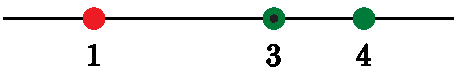
\includegraphics{convDiv.pdf}
\end{center}
\end{efig}
Can we say more about the convergence and/or divergence of the series for other values of $x$? Yes!

Let us think about the radius of convergence, $R$, of the series. We know that it must exist and the information we have
been given allows us to bound $R$. Recall that
\begin{itemize}
\item the series converges at $x$ provided that $|x-3|<R$ and
\item the series diverges at $x$ if $|x-3|>R$.
\end{itemize}
We have been told that
\begin{itemize}
\item the series converges when $x=4$, which tells us that
\begin{itemize}
\item[$\circ$] $x=4$ cannot obey $|x-3|>R$ so
\item[$\circ$] $x=4$ must obey $|x-3|\le R$, \ \ i.e. $|4-3|\le R$,\ \
 i.e. $R\ge 1$
\end{itemize}
\item the series diverges when $x=1$ so we also know that
\begin{itemize}
\item[$\circ$] $x=1$ cannot obey $|x-3|<R$ so
\item[$\circ$] $x=1$ must obey $|x-3|\ge R$, i.e. $|1-3|\ge R$, i.e. $R\le 2$
\end{itemize}
\end{itemize}
We still don't know $R$ exactly. But we do know that $1\le R\le 2$.
Consequently,
\begin{itemize}
\item since $1$ is the smallest that $R$ could be, the series
certainly converges at $x$ if $|x-3|<1$, i.e. if $2<x<4$ and
\item since $2$ is the largest that $R$ could be, the series
certainly diverges at $x$ if $|x-3|>2$, i.e. if $x>5$ or if $x<1$.
\end{itemize}
The following figure provides a resume of all of this convergence
data --- there is convergence at green $x$'s and divergence at
red $x$'s.
\begin{efig}
\begin{center}
     
\includegraphics{convDivB.pdf}
\end{center}
\end{efig}
Notice that from the data given we cannot say anything about the
convergence or divergence of the series on the
intervals $(1,2]$ and $(4,5]$.

\noindent
One lesson that we can derive from this example is that,
\begin{itemize}
\item
if a series has centre $c$ and converges at $a$,
\item
then it also converges at all points between $c$ and $a$, as well
as at all points of distance strictly less than $|a-c|$ from $c$
on the other side of $c$ from $a$.
\end{itemize}
\end{eg}



%%%%%%%%%%%%%%%%%%%%%%%%%%%%%%%%%%%%%%%%%%%%%%%%%%%%%%%%%%%%
\subsection{Working With Power Series}
%%%%%%%%%%%%%%%%%%%%%%%%%%%%%%%%%%%%%%%%%%%%%%%%%%%%%%%%%%%%

Just as we have done previously with limits, differentiation
and integration, we can construct power series representations
of more complicated functions by using those of simpler functions.
Here is a theorem that helps us to do so.
\begin{theorem}[Operations on Power Series]\label{thm:SRpsops}
Assume that the functions $f(x)$ and $g(x)$ are given by the power series
\begin{equation*}
f(x) = \sum_{n=0}^\infty A_n (x-c)^n \qquad
g(x) = \sum_{n=0}^\infty B_n (x-c)^n
\end{equation*}
for all $x$ obeying $|x-c|<R$. In particular, we are assuming that both
power series have radius of convergence at least
$R$. Also let $K$ be a constant. Then
\begin{align*}
f(x)+g(x)   &= \sum_{n=0}^\infty [A_n+B_n]\, (x-c)^n \\
  Kf(x)     &= \sum_{n=0}^\infty K\, A_n\, (x-c)^n \\
(x-c)^Nf(x) &= \sum_{n=0}^\infty A_n\, (x-c)^{n+N}
                         \quad\text{for any integer $N\ge 1$}\\
           &= \sum_{k=N}^\infty A_{k-N}\, (x-c)^k
                         \quad\text{where $k=n+N$}\\
f'(x)     &= \sum_{n=0}^\infty A_n\, n\,(x-c)^{n-1}
           = \sum_{n=1}^\infty A_n\, n\,(x-c)^{n-1} \\
\int_c^x f(t)\ dt &= \sum_{n=0}^\infty A_n \frac{(x-c)^{n+1}}{n+1} \\
\int  f(x)\ \dee{x} &= \bigg[\sum_{n=0}^\infty A_n \frac{(x-c)^{n+1}}{n+1}\bigg]+C
\quad\text{with $C$ an arbitrary constant}
\end{align*}
for all $x$ obeying $|x-c|<R$.

In particular the radius of convergence of each of the six power
series on the right hand sides is at least $R$. In fact, if $R$
is the radius of convergence of $\sum\limits_{n=0}^\infty A_n (x-c)^n$,
then $R$ is also the radius of convergence of all of the above
right hand sides, with the possible exceptions of
$\sum\limits_{n=0}^\infty [A_n+B_n]\, (x-c)^n$ and
$\sum\limits_{n=0}^\infty KA_n\, (x-c)^n$ when $K=0$.
\end{theorem}

\begin{eg}
The last statement of Theorem \ref{thm:SRpsops} might seem a little odd,
but consider the following two power series centred at $0$:
\begin{align*}
  \sum_{n=0}^\infty 2^n x^n & \text{ and } \sum_{n=0}^\infty (1-2^n) x^n.
\end{align*}
The ratio test tells us that they both have radius of convergence $R=\frac{1}{2}$. However their sum is
\begin{align*}
  \sum_{n=0}^\infty 2^n x^n + \sum_{n=0}^\infty (1-2^n) x^n
  &= \sum_{n=0}^\infty x^n
\end{align*}
which has the larger radius of convergence $1$.

A more extreme example of the same phenomenon is supplied by the two series
\begin{align*}
  \sum_{n=0}^\infty 2^n x^n & \text{ and } \sum_{n=0}^\infty (-2^n) x^n.
\end{align*}
They are both geometric series with radius of convergence $R=\frac{1}{2}$.
But their sum is
\begin{align*}
  \sum_{n=0}^\infty 2^n x^n + \sum_{n=0}^\infty (-2^n) x^n
  &= \sum_{n=0}^\infty (0)x^n
\end{align*}
which has radius of convergence $+\infty$.
\end{eg}

We'll now use this theorem to build power series representations
for a bunch of functions out of the one simple power
series representation that we know --- the geometric series
\begin{equation*}
\frac{1}{1-x} = \sum_{n=0}^\infty x^n\qquad \text{for all $|x|<1$}
\end{equation*}

\begin{eg}[$\frac{1}{1-x^2}$]\label{eg:SRpsrepAA}
Find a power series representation for $\frac{1}{1-x^2}$.

\soln
The secret to finding power series representations for a good many functions
is to manipulate them into a form in which $\frac{1}{1-y}$ appears
and use the geometric series representation
$\frac{1}{1-y} = \sum_{n=0}^\infty y^n$. We have deliberately renamed
the variable to $y$ here --- it does not have to be $x$. We can use that
strategy to find a power series expansion for $\frac{1}{1-x^2}$ --- we
just have to recognize that $\frac{1}{1-x^2}$ is the same as
$\frac{1}{1-y}$ if we set $y$ to $x^2$.
\begin{alignat*}{3}
\frac{1}{1-x^2} &= \frac{1}{1-y}\bigg|_{y=x^2}\quad &
             &=\bigg[\sum_{n=0}^\infty y^n
                                     \bigg]_{y=x^2}
                   \quad\text{if $|y|<1$, i.e. $|x|<1$} \\
             &= \sum_{n=0}^\infty {\big(x^2\big)}^n &
             &= \sum_{n=0}^\infty x^{2n} \\
             &= 1+x^2+x^4+x^6  +\cdots \hidewidth
\end{alignat*}
This is a perfectly good power series. There is nothing wrong with the
power of $x$ being $2n$. (This just means that the coefficients of all odd powers of $x$ are zero.) In fact, you should try to always write power
series in forms that are as easy to understand as possible. The geometric
series that we used at the end of the first line converges for
\begin{align*}
|y|<1
\iff  \big|x^2\big|<1
\iff |x|<1
\end{align*}
So our power series has radius of convergence $1$ and interval of
convergence $-1<x<1$.
\end{eg}



\goodbreak
\begin{eg}[$\frac{x}{2+x^2}$]\label{eg:SRpsrepA}
Find a power series representation for $\frac{x}{2+x^2}$.

\soln
This example is just a more algebraically involved variant of
the last one. Again, the strategy is to manipulate $\frac{x}{2+x^2}$
into a form in which $\frac{1}{1-y}$ appears.
\begin{alignat*}{3}
\frac{x}{2+x^2} &= \frac{x}{2}\ \frac{1}{1+\nicefrac{x^2}{2}}
             =\ \frac{x}{2}\ \frac{1}{1-\big({-}\nicefrac{x^2}{2}\big)}
             \qquad \text{set $-\frac{x^2}{2}=y$} \\
             &= \frac{x}{2}\ \frac{1}{1-y}\bigg|_{y=-\frac{x^2}{2}}
             = \frac{x}{2}\ \bigg[\sum_{n=0}^\infty y^n
                                     \bigg]_{y=-\frac{x^2}{2}}
                   \quad\text{if $|y|<1$} \\
             &= \frac{x}{2}\ \sum_{n=0}^\infty {\Big(-\frac{x^2}{2}\Big)}^n
             =\ \frac{x}{2}\ \sum_{n=0}^\infty \frac{(-1)^n}{2^n}x^{2n}
             = \sum_{n=0}^\infty \frac{(-1)^n}{2^{n+1}}x^{2n+1}
                \quad\text{by Theorem \ref{thm:SRpsops}, twice} \\
             &= \frac{x}{2} - \frac{x^3}{4} + \frac{x^5}{8}-\frac{x^7}{16}
                 +\cdots
\end{alignat*}
The geometric series that we used in the second line converges when
\begin{align*}
|y|<1
\iff  \big|{-}\nicefrac{x^2}{2}\big|<1
\iff  |x|^2<2
\iff |x|<\sqrt{2}
\end{align*}
So the given power series has radius of convergence $\sqrt{2}$ and interval of
convergence $-\sqrt{2}<x<\sqrt{2}$.
\end{eg}

\goodbreak
\begin{eg}[Nonzero centre]\label{eg:SRpsrepAAA}
Find a power series representation for $\frac{1}{5-x}$ with centre
$3$.

\soln
The new wrinkle in this example is the requirement that the centre
be $3$. That the centre is to be $3$ means that we need a power series
in powers of $x-c$, with $c=3$.  So we are looking for a power
series of the form $\sum_{n=0}^\infty A_n(x-3)^n$. The easy way
to find such a series is to force an $x-3$ to appear by adding
and subtracting a $3$.
\begin{align*}
\frac{1}{5-x}
=\frac{1}{5-(x-3)-3}
=\frac{1}{2-(x-3)}
\end{align*}
Now we continue, as in the last example, by manipulating $\frac{1}{2-(x-3)}$
into a form in which $\frac{1}{1-y}$ appears.
\begin{alignat*}{3}
\frac{1}{5-x}
=\frac{1}{2-(x-3)} &= \frac{1}{2}\ \frac{1}{1-\frac{x-3}{2}}
             \qquad \text{set $\frac{x-3}{2}=y$} \\
             &= \frac{1}{2}\ \frac{1}{1-y}\bigg|_{y=\frac{x-3}{2}}
             = \frac{1}{2}\ \bigg[\sum_{n=0}^\infty y^n
                                     \bigg]_{y=\frac{x-3}{2}}
                   \quad\text{if $|y|<1$} \\
             &= \frac{1}{2}\ \sum_{n=0}^\infty {\Big(\frac{x-3}{2}\Big)}^n
             = \sum_{n=0}^\infty \frac{(x-3)^n}{2^{n+1}} \\
             &= \frac{x-3}{2} + \frac{(x-3)^2}{4} + \frac{(x-3)^3}{8}
                 +\cdots
\end{alignat*}
The geometric series that we used in the second line converges when
\begin{align*}
|y|<1
\iff  \Big|\frac{x-3}{2}\Big|<1
\iff  |x-3|<2
\iff -2<x-3<2
\iff 1<x<5
\end{align*}
So the power series has radius of convergence $2$ and interval of
convergence $1<x<5$.
\end{eg}


In the previous two examples, to construct a new series from an
existing series, we replaced $x$ by a simple function. The following
theorem gives us some more (but certainly not all) commonly
used substitutions.


\begin{theorem}[Substituting in a Power Series]\label{thm:SRpsSub}
Assume that the function $f(x)$ is given by the power
series
\begin{equation*}
f(x) = \sum_{n=0}^\infty A_n x^n
\end{equation*}
for all $x$ in the interval $I$. Also let $K$ and $k$ be real constants. Then
\begin{align*}
f\big(Kx^k\big)   &= \sum_{n=0}^\infty A_nK^n\, x^{kn} \\
\end{align*}
whenever $Kx^k$ is in $I$. In particular, if $\sum_{n=0}^\infty A_n x^n$
has radius of convergence $R$, $K$ is nonzero and $k$ is a natural number,
then $\sum_{n=0}^\infty A_nK^n\, x^{kn}$ has radius of convergence
$\root{k}\of{R/|K|}$.
\end{theorem}


\begin{eg}[$\frac{1}{(1-x)^2}$]\label{eg:SRpsrepB}
Find a power series representation for $\frac{1}{(1-x)^2}$.

\soln
Once again the trick is to express $\frac{1}{(1-x)^2}$ in terms of
$\frac{1}{1-x}$. Notice that
\begin{align*}
\frac{1}{(1-x)^2} &= \diff{}{x}\left\{\frac{1}{1-x}\right\} \\
             &= \diff{}{x} \left\{\sum_{n=0}^\infty x^n \right\}\\
             &= \sum_{n=1}^\infty nx^{n-1}
             \qquad\text{by Theorem \ref{thm:SRpsops}}
\end{align*}
Note that the $n=0$ term has disappeared because, for $n=0$,
\begin{equation*}
\diff{}{x} x^n = \diff{}{x} x^0 = \diff{}{x} 1= 0
\end{equation*}
Also note that the radius of convergence of this series is one. We can
see this via Theorem~\ref{thm:SRpsops}. That theorem tells us that
the radius of convergence of a power series is not changed by
differentiation --- and since $\sum_{n=0}^\infty x^n$ has radius
of convergence one, so too does its derivative.

Without much more work we can determine the interval of convergence
by testing at $x=\pm 1$. When $x=\pm 1$ the terms of the series do not
go to zero as $n \to \infty$ and so, by the divergence test, the series
does not converge there. Hence the interval of convergence for the
series is $-1 < x < 1$.
\end{eg}
Notice that, in this last example, we differentiated a known series to get
to our answer. As per Theorem~\ref{thm:SRpsops}, the radius of convergence
didn't change. In addition, in this particular example, the interval
of convergence didn't change. This is not always the case.
Differentiation of some series causes the interval of convergence to shrink.
In particular the differentiated series may no longer be convergent
at the end points of the interval\footnote{Consider the power series
$\sum_{n=1}^\infty \frac{x^n}{n}$. We know that its interval of
convergence is $-1 \leq x < 1$. (Indeed see the next example.) When
we differentiate the series we get the geometric series
$\sum_{n=0}^\infty x^n$ which has interval of convergence $-1<x<1$. }. Similarly, when we integrate a power series the radius of convergence is
unchanged, but the interval of convergence may expand to include one or both ends, as illustrated by the next example.


\begin{eg}[$\log (1+x)$]\label{eg:SRpsrepC}
Find a power series representation for $\log (1+x)$.

\soln
Recall that $\diff{}{x}\log (1+x) = \frac{1}{1+x}$ so that
$\log(1+t)$ is an antiderivative of $\frac{1}{1+t}$ and
\begin{align*}
\log(1+x)\ &=\ \int_0^x \frac{dt}{1+t}
             \ =\  \int_0^x\Big[\sum_{n=0}^\infty (-t)^n\Big]\ dt \\
             &=\  \sum_{n=0}^\infty \int_0^x (-t)^n\ dt
             \qquad\text{by Theorem \ref{thm:SRpsops}}\\
             &=\ \sum_{n=0}^\infty (-1)^n\frac{x^{n+1}}{n+1} \\
             &=\ x-\frac{x^2}{2}+\frac{x^3}{3}-\frac{x^4}{4}+\cdots
\end{align*}
Theorem \ref{thm:SRpsops} guarantees that the radius of convergence is
exactly one (the radius of convergence of the geometric series
$\sum_{n=0}^\infty (-t)^n$) and that
\begin{align*}
\log(1+x) = \sum_{n=0}^\infty (-1)^n\frac{x^{n+1}}{n+1}
\qquad\text{for all}\quad -1<x<1
\end{align*}
When $x=-1$ our series reduces to
$\sum_{n=0}^\infty \frac{-1}{n+1}$, which is (minus) the harmonic
series and so diverges. That's no surprise --- $\log(1+(-1))
=\log 0=-\infty$.  When $x=1$, the series
converges by the alternating series test. It is possible to prove, by continuity, though we won't do so here, that the sum is $\log 2$.
So the interval of convergence is $-1<x\le 1$.
\intremark{
Set, for $-1<x\le 1$ and $N\in\bbbn$
\begin{align*}
S_N(x) = \sum_{n=0}^N (-1)^n\frac{x^{n+1}}{n+1}
\qquad
S(x) = \sum_{n=0}^\infty (-1)^n\frac{x^{n+1}}{n+1}
\end{align*}
By the alternating series test, for all $0\le x\le 1$,
\begin{equation*}
\big|S(x) - S_N(x)\big| \le \frac{1}{N+2}
\end{equation*}
So $S_N$ converges uniformly on $[0,1]$ to $S(x)$. As every $S_N$
is continuous on $[0,1]$, $S(x)$ is also continuous on $[0,1]$.
So $S(x) = \log(1+x)$ on $(-1,1]$.
}
\end{eg}


\begin{eg}[$\arctan x$]\label{eg:SRpsrepD}
Find a power series representation for $\arctan x$.

\soln
Recall that $\diff{}{x}\arctan x = \frac{1}{1+x^2}$ so that
$\arctan t$ is an antiderivative of $\frac{1}{1+t^2}$ and
\begin{align*}
\arctan x\ &=\ \int_0^x \frac{dt}{1+t^2}
             \ =\  \int_0^x\Big[\sum_{n=0}^\infty {(-t^2)}^n\Big]\ dt
             \ =\  \sum_{n=0}^\infty \int_0^x (-1)^n t^{2n}\ dt \\
             &=\ \sum_{n=0}^\infty (-1)^n\frac{x^{2n+1}}{2n+1} \\
             &=x -\frac{x^3}{3} +\frac{x^5}{5}-\cdots
\end{align*}
Theorem \ref{thm:SRpsops} guarantees that the radius of convergence is
exactly one (the radius of convergence of the geometric series
$\sum_{n=0}^\infty (-t^2)^n$) and that
\begin{align*}
\arctan x\ &=\ \sum_{n=0}^\infty (-1)^n\frac{x^{2n+1}}{2n+1}
\qquad\text{for all $-1<x<1$}
\end{align*}
When $x=\pm 1$, the series converges by the alternating series test.
So the interval of convergence is $-1\le x\le 1$.
It is possible to prove, though once again we won't do so here,
that when $x=\pm 1$, the series
$\sum_{n=0}^\infty (-1)^n\frac{x^{2n+1}}{2n+1}$
converges to the value of the left hand side, $\arctan x$, at $x=\pm 1$.
That is, to $\arctan(\pm 1)=\pm \frac{\pi}{4}$.
\end{eg}

The operations on power series dealt with in Theorem~\ref{thm:SRpsops}
are fairly easy to apply. Unfortunately taking the product, ratio
or composition of two power series is more involved and is beyond
the scope of this course\footnote{As always, a quick visit to your
favourite search engine will direct the interested reader to more information.}.
Unfortunately Theorem~\ref{thm:SRpsops} alone will not get us
power series representations of many of our standard  functions
(like  $e^x$ and $\sin x$).  Fortunately we can find such
representations by extending Taylor polynomials\footnote{Now is a good
time to review your notes from last term, though  we'll give you a
whirlwind review over the next page or two.} to Taylor series.


\intremark{%%% INTERNAL REMARK - series multiplication and division
\begin{theorem}[More Operations on Power Series]\label{thm:SRmoreOps}
Assume that the functions $f(x)$ and $g(x)$ are given by power series
centred on $c$  with radius of convergence at least $R$.
\begin{enumerate}[(a)]
\item Then $f(x) g(x)$ has a power series expansion, centred on $c$ with radius
of convergence at least $R$.
 \item If $g(c)\ne 0$, then $\frac{f(x)}{g(x)}$ has a
power series expansion, centred on $c$ with radius
of convergence at least $0$.
\end{enumerate}
\end{theorem}

\begin{eg}[${[\log(1+x)]}^2$]\label{eg:SRmult}
\begin{align*}
{[\log(1+x)]}^2
&=\Big\{x-\frac{x^2}{2}+\frac{x^3}{3}+\cdots\Big\}
  \Big\{x-\frac{x^2}{2}+\frac{x^3}{3}+\cdots\Big\} \\
&=\kern15pt x\Big\{x-\frac{x^2}{2}+\frac{x^3}{3}+\cdots\Big\} \\
  &\kern10pt
    -\frac{x^2}{2}\Big\{x-\frac{x^2}{2}+\frac{x^3}{3}+\cdots\Big\} \\
  &\kern10pt
    +\frac{x^3}{3}\Big\{x-\frac{x^2}{2}+\frac{x^3}{3}+\cdots\Big\}-\cdots \\
&= x^2-\frac{x^3}{2}+\frac{x^4}{3}+\cdots \\
&\kern27pt    -\frac{x^3}{2}+\frac{x^4}{4}+\cdots \\
&\kern56pt       +\frac{x^4}{3}+\cdots \\
&= x^2-x^3+\frac{11}{12}x^4+\cdots
\end{align*}

\end{eg}

\begin{eg}[$\tan x$]\label{eg:SRdiv}
In this example we find the first few terms of
\begin{equation*}
\tan x=\frac{\sin x}{\cos x}=\frac{x-\frac{x^3}{3!}+\frac{x^5}{5!}-\cdots}
                                   {1-\frac{x^2}{2!}+\frac{x^4}{4!}-\cdots}
\end{equation*}
by long division
\issue{INCOMPLETE}
\end{eg}
} %%% END INTERNAL REMARK - series multiplication and division

%%%%%%%%%%%%%%%%%%%%%%%%%%%%%%%%%%%%%%%%%%%%%%%%%%%%%%%%%%%%
\section{Taylor Series}
%%%%%%%%%%%%%%%%%%%%%%%%%%%%%%%%%%%%%%%%%%%%%%%%%%%%%%%%%%%%

%%%%%%%%%%%%%%%%%%%%%%%%%%%%%
\subsection{Extending Taylor Polynomials}
%%%%%%%%%%%%%%%%%%%%%%%%%%%%%

Recall\footnote{Please review your notes from last term if this material
is feeling a little unfamiliar.} that Taylor polynomials provide a
hierarchy of approximations to a given function $f(x)$ near a given point $a$.
Typically, the quality of these approximations improves as we move
up the hierarchy.
\begin{itemize}
\item The crudest approximation is the constant approximation $f(x)\approx f(a)$.
\item Then comes the linear, or tangent line, approximation $f(x)\approx f(a) + f'(a)\,(x-a)$.

\item Then comes the quadratic approximation
\begin{equation*}
f(x)\approx f(a) + f'(a)\,(x-a) +\frac{1}{2} f''(a)\,(x-a)^2
\end{equation*}

\item In general, the Taylor polynomial of degree $n$, for the
function $f(x)$, about the expansion point $a$, is the
polynomial, $T_n(x)$,  determined by the requirements that $f^{(k)}(a) = T_n^{(k)}(a)$ for all $0\le k \le n$. That
is, $f$ and $T_n$ have the same derivatives at $a$, up to order $n$.
Explicitly,
\begin{align*}
f(x) \approx T_n(x) &= f(a) + f'(a)\,(x-a) +\frac{1}{2} f''(a)\,(x-a)^2
%+\frac{1}{3!} f^{(3)}(a)\,(x-a)^3
+\cdots+\frac{1}{n!} f^{(n)}(a)\,(x-a)^n \\
&=\sum_{k=0}^n\frac{1}{k!} f^{(k)}(a)\,(x-a)^k
\end{align*}
\end{itemize}
These are, of course, approximations --- often very good approximations near $x=a$ --- but still just approximations. One might hope that if we let
the degree, $n$, of the approximation go to infinity then the error in
the approximation might go to zero. If that is the case then the
``infinite'' Taylor polynomial would be an exact representation
of the function. Let's see how this might work.


Fix a real number $a$ and suppose that all derivatives of the function $f(x)$ exist. Then, we saw in (\eref{CLP1}{eq:taylorErrorN}) of the CLP-1 text that, for any natural number $n$,
\begin{impeqn}\label{eq:TaylorPolyPlusError}
\begin{align*}
f(x) &=T_n(x) +E_n(x)
\end{align*}
\end{impeqn}
\noindent where $T_n(x)$ is the Taylor polynomial of degree $n$
for the function $f(x)$ expanded about $a$, and  $E_n(x)=f(x)-T_n(x)$
is the error in the approximation $f(x) \approx T_n(x)$. 
The Taylor polynomial\footnote{Did you
take a quick look at your notes?} is given by the formula
%
\resetimpsubeqn %use this to reset the impsubeqn counter.
\begin{impsubeqn}\label{eq:TaylorPolyPlusError_a}
\begin{align*}
T_n(x)&=f(a)+f'(a)\,(x-a)+\cdots+\tfrac{1}{n!}f^{(n)}(a)\, (x-a)^n
\end{align*}
\end{impsubeqn}
\noindent while the error satisfies\footnote{This is probably the most commonly used formula for the error. But there is another fairly commonly used formula.  It, and some less commonly used formulae, are given in the next (optional) subsection ``More about the Taylor Remainder''.}
\begin{impsubeqn}\label{eq:TaylorPolyPlusError_b}
\begin{align*}
E_n(x)=\tfrac{1}{(n+1)!}f^{(n+1)}(c)\, (x-a)^{n+1}
\end{align*}
\end{impsubeqn}
\noindent for some $c$ strictly between $a$ and $x$. Note that we typically
do not know the value of $c$ in the formula for the error.
Instead we use the bounds on $c$ to find bounds on $f^{(n+1)}(c)$ and
so bound the error\footnote{The discussion here is only supposed to
jog your memory. If it is feeling insufficiently jogged, then
please look at your notes from last term.}.

In order for our Taylor polynomial to be an exact representation of
the function $f(x)$ we need the error $E_n(x)$ to be zero.
This will not happen when $n$ is finite unless $f(x)$ is a
polynomial. However it can happen in the limit as $n \to \infty$,
and in that case we can write $f(x)$ as the limit
\begin{equation*}
f(x)=\lim_{n\rightarrow\infty} T_n(x)
=\lim_{n\rightarrow\infty} \sum_{k=0}^n \tfrac{1}{k!}f^{(k)}(a)\, (x-a)^k
\end{equation*}
This is really a limit of partial sums, and so we can write
\begin{align*}
f(x)=\sum_{k=0}^\infty \tfrac{1}{k!}f^{(k)}(a)\, (x-a)^k
\end{align*}
which is a power series representation of the function. Let us
formalise this in a definition.
\begin{defn}[Taylor series]\label{defn:taylorSeries}
The Taylor series for the function $f(x)$ expanded around $a$
is the power series
\begin{align*}
\sum_{n=0}^\infty \tfrac{1}{n!}f^{(n)}(a)\, (x-a)^n
\end{align*}
When $a=0$ it is also called the Maclaurin series of $f(x)$. If 
$\lim_{n\rightarrow\infty}E_n(x)=0$, then
\begin{align*}
f(x)=\sum_{n=0}^\infty \tfrac{1}{n!}f^{(n)}(a)\, (x-a)^n
\end{align*}
\end{defn}
\noindent
Demonstrating that, for a given function, $\lim_{n\rightarrow\infty}E_n(x)=0$
can be difficult.
%This definition hides the discussion of whether or not $E_n(x) \to 0$
%as $n\rightarrow\infty$ within the caveat ``provided the series converges''.
%Demonstrating that for a given function can be difficult, 
but for many of the standard functions you are used to dealing with, 
it turns out to be pretty easy. Let's compute a few Taylor series and see 
how we do it.


\begin{eg}[Exponential Series]\label{eg:expSeries}
Find the Maclaurin series for $f(x)=e^x$.

\soln Just as was the case for computing Taylor polynomials, we need
to compute the derivatives of the function at the
particular choice of $a$. Since we are asked for a Maclaurin series,
$a=0$. So now we just need to find
$f^{(k)}(0)$ for all integers $k\ge 0$.

We know that $\diff{}{x}e^x = e^x$ and so
\begin{align*}
  e^x &= f(x) = f'(x) = f''(x) = \cdots = f^{(k)}(x) = \cdots & \text{which gives}\\
  1 &= f(0) = f'(0) = f''(0) = \cdots = f^{(k)}(0) = \cdots.
\end{align*}
Equations~\eqref{eq:TaylorPolyPlusError} and~\eqref{eq:TaylorPolyPlusError_a} then give us
\begin{align*}
e^x=f(x)&=
1+x+\frac{x^2}{2!}+\cdots+\frac{x^n}{n!}+E_n(x)
\end{align*}
We shall see, in the optional Example \ref{eg:expSeriesB} below, that,
for any fixed $x$, $\lim\limits_{n\rightarrow\infty}E_n(x)=0$.
Consequently, for all $x$,
\begin{equation*}%\label{eq:TaylorSeriesExp}
e^x=\lim_{n\rightarrow\infty}\Big[1 +x + \frac{1}{2} x^2
     +\frac{1}{3!} x^3+\cdots+\frac{1}{n!} x^n\Big]
    =\sum_{n=0}^\infty \frac{1}{n!}x^n
\end{equation*}
\end{eg}


We have now seen power series representations for the functions
\begin{align*}
  \frac{1}{1-x} && \frac{1}{(1-x)^2} && \log(1+x) && \arctan(x) && e^x.
\end{align*}
We do not think that you, the reader, will be terribly surprised to see
that we develop series for sine and cosine next.

\begin{eg}[Sine and Cosine Series]\label{eg:sincosSeries}
The trigonometric functions $\sin x$ and $\cos x$ also have widely used
Maclaurin series expansions (i.e. Taylor series expansions about $a=0$).
To find them, we first compute all derivatives at general $x$.
\begin{equation*}%\label{eq:sinCosDerivs}
\begin{aligned}
f(x)&=\sin x &
f'(x)&=\cos x &
f''(x)&=-\sin x &
f^{(3)}(x)&=-\cos x &
f^{(4)}(x)&=\sin x & \cdots\\
g(x)&=\cos x &
g'(x)&=-\sin x &
g''(x)&=-\cos x &
g^{(3)}(x)&=\sin x &
g^{(4)}(x)&=\cos x & \cdots
\end{aligned}
\end{equation*}
%We see that the second derivative is just $-1$ times the original function,
%and the fourth derivative is the same as the original function.
%\begin{align*}
%  \ddiff{2}{y}{x} &= -y(x) & \text{ so } && \ddiff{4}{y}{x} &= y(x).
%\end{align*}
%Consequently the derivatives give a pattern of period 4. It is worth
%noting here that the function $y(x)=e^x$ also satisfies the second
%differential equation --- we will explore this a little more in
%an optional subsection.
%
Now set $x=a=0$.
\begin{equation*}%\label{eq:sinCosDerivsZero}
\begin{aligned}
f(x)&=\sin x &
f(0)&=0 &
f'(0)&=1 &
f''(0)&=0 &
f^{(3)}(0)&=-1 &
f^{(4)}(0)&=0 & \cdots\\
g(x)&=\cos x &
g(0)&=1 &
g'(0)&=0 &
g''(0)&=-1 &
g^{(3)}(0)&=0 &
g^{(4)}(0)&=1 & \cdots
\end{aligned}
\end{equation*}
For $\sin x$, all even numbered derivatives (at $x=0$) are zero,
while the odd numbered derivatives alternate between $1$ and $-1$.
Very similarly, for $\cos x$, all odd numbered derivatives (at $x=0$) are zero,
while the even numbered derivatives alternate between $1$ and $-1$.
So, the Taylor polynomials that best approximate $\sin x$ and $\cos x$
near $x=a=0$ are
\begin{align*}
\sin x &\approx x-\tfrac{1}{3!}x^3+\tfrac{1}{5!}x^5-\cdots\\
\cos x &\approx 1-\tfrac{1}{2!}x^2+\tfrac{1}{4!}x^4-\cdots
\end{align*}
We shall see, in the optional Example \ref{eg:sincosSeriesB}
below, that, for both $\sin x$ and $\cos x$,
we have $\lim\limits_{n\rightarrow\infty}E_n(x)=0$ so that
\begin{align*}
f(x)&=\lim_{n\rightarrow\infty}\Big[f(0)+f'(0)\,x+\cdots
                +\tfrac{1}{n!}f^{(n)}(0)\, x^n\Big] \\
g(x)&=\lim_{n\rightarrow\infty}\Big[g(0)+g'(0)\,x+\cdots
                +\tfrac{1}{n!}g^{(n)}(0)\, x^n\Big]
\end{align*}
Reviewing the patterns we found in the derivatives, we conclude that,
for all $x$,
\begin{equation*}%\label{eq:TaylorSeriesSinCos}
\begin{alignedat}{2}
\sin x &= x-\tfrac{1}{3!}x^3+\tfrac{1}{5!}x^5-\cdots&
       &=\sum_{n=0}^\infty(-1)^n\tfrac{1}{(2n+1)!}x^{2n+1}\\
\cos x &= 1-\tfrac{1}{2!}x^2+\tfrac{1}{4!}x^4-\cdots&
       &=\sum_{n=0}^\infty(-1)^n\tfrac{1}{(2n)!}x^{2n}
\end{alignedat}
\end{equation*}
and, in particular, both of the series on the right hand sides converge
for all $x$.

We could also test for convergence of the series using
the ratio test. Computing the ratios of successive terms in these
two series gives us
\begin{align*}
  \left| \frac{A_{n+1}}{A_n} \right|
        &= \frac{|x|^{2n+3}/(2n+3)!}{|x|^{2n+1}/(2n+1)!}
         = \frac{|x|^2}{(2n+3)(2n+2)} \\
  \left| \frac{A_{n+1}}{A_n} \right|
        &= \frac{|x|^{2n+2}/(2n+2)!}{|x|^{2n}/(2n)!}
         = \frac{|x|^2}{(2n+2)(2n+1)}
\end{align*}
for sine and cosine respectively. Hence as $n \to \infty$ these ratios go to zero and consequently both series are
convergent for all $x$. (This is very similar to what was observed in Example~\ref{eg:PWRb}.)
\end{eg}


We have developed power series representations for a number of important
functions\footnote{The reader might ask whether or not we will give
the series for other trigonometric functions or their inverses. While
the tangent function has a perfectly well defined series, its
coefficients are not as simple as those of the series we have
seen --- they form a sequence of numbers known (perhaps unsurprisingly)
as the ``tangent numbers''. They, and the related Bernoulli numbers,
have many interesting properties, links to which the interested reader
can find with their favourite search engine. The Maclaurin series for
inverse sine is
\begin{align*}
  \arcsin(x) &= \sum_{n=0}^\infty \frac{4^{-n}}{2n+1}\frac{(2n)!}{(n!)^2} x^{2n+1}
\end{align*}
which is quite tidy, but proving it is beyond the scope of the course.
}
. Here is a theorem that summarizes
them.
\begin{theorem}\label{thm:SRimportantTaylorSeries}
\begin{alignat*}{5}
e^x &= \sum_{n=0}^\infty\frac{x^n}{n!}
    &&= 1 +x + \frac{1}{2!} x^2 +\frac{1}{3!} x^3+\cdots
    &&\qquad\text{for all $-\infty<x<\infty$} \\
\sin(x) &= \sum_{n=0}^\infty(-1)^n\frac{1}{(2n+1)!}x^{2n+1}
    &&= x-\frac{1}{3!}x^3+\frac{1}{5!}x^5-\cdots
    &&\qquad\text{for all $-\infty<x<\infty$} \\
\cos(x) &= \sum_{n=0}^\infty(-1)^n\frac{1}{(2n)!}x^{2n}
    &&= 1-\frac{1}{2!}x^2+\frac{1}{4!}x^4-\cdots
    &&\qquad\text{for all $-\infty<x<\infty$} \\
\frac{1}{1-x} &= \sum_{n=0}^\infty x^n
    &&= 1 + x+ x^2 + x^3 + \cdots
    &&\qquad\text{for all $-1<x<1$} \\
\log(1+x) &= \sum_{n=0}^\infty (-1)^n\frac{x^{n+1}}{n+1}
     &&= x-\frac{x^2}{2}+\frac{x^3}{3}-\frac{x^4}{4}+\cdots
    &&\qquad\text{for all $-1<x\le 1$} \\
\arctan x &=  \sum_{n=0}^\infty (-1)^n\frac{x^{2n+1}}{2n+1}
    &&= x -\frac{x^3}{3} +\frac{x^5}{5}-\cdots
    &&\qquad\text{for all $-1\le x\le 1$}
\end{alignat*}
\end{theorem}
Notice that the series for sine and cosine sum to something that looks very similar to the series for $e^x$:
\begin{align*}
  \sin(x)+\cos(x) &= \left(x-\frac{1}{3!}x^3+\frac{1}{5!}x^5-\cdots\right)
  +\left(1-\frac{1}{2!}x^2+\frac{1}{4!}x^4-\cdots\right)\\
  &= 1 + x - \frac{1}{2!}x^2 - \frac{1}{3!}x^3 + \frac{1}{4!}x^4 + \frac{1}{5!}x^5 - \cdots\\
  e^x
  &= 1 + x + \frac{1}{2!}x^2 + \frac{1}{3!}x^3 + \frac{1}{4!}x^4 + \frac{1}{5!}x^5 + \cdots
\end{align*}
So both series have coefficients with the same absolute value
(namely $\frac{1}{n!}$), but there are differences in
sign\footnote{Warning: antique sign--sine pun. No doubt the reader
first saw it many years syne.}.
This is not a coincidence and we direct the interested reader to the optional Section \ref{sec:Euler} where will show how these series are linked through $\sqrt{-1}$.


\begin{eg}[Optional --- Why  $\sum_{n=0}^\infty \frac{1}{n!}x^n$ is $e^x$.]
                                         \label{eg:expSeriesB}

We have already seen, in Example \ref{eg:expSeries}, that
\begin{equation*}%\label{eq:expTaylorC}
e^x
= 1+x+\frac{x^2}{2!}+\cdots+\frac{x^n}{n!}+E_n(x)
\end{equation*}
By (\ref{eq:TaylorPolyPlusError_b})
\begin{equation*}
E_n(x) = \frac{1}{(n+1)!}e^c x^{n+1}
\end{equation*}
for some (unknown) $c$ between $0$ and $x$. Fix any real number
$x$. We'll now show that $E_n(x)$ converges to zero as $n\rightarrow\infty$.


To do this we need get bound the size of $e^c$, and to do this, consider what happens if $x$ is positive or negative.
\begin{itemize}
 \item If $x<0$ then $x \leq c \leq 0$ and hence $e^x \leq e^c \leq e^0=1$.
 \item On the other hand, if $x\geq 0$ then $0\leq c \leq x$ and so $1=e^0 \leq e^c \leq e^x$.
\end{itemize}
In either case we have that $0 \leq e^c \leq 1+e^x$. Because of this the error term
\begin{equation*}
|E_n(x)|=\Big|\frac{e^c}{(n+1)!}x^{n+1}\Big|
\le [e^x+1]\frac{|x|^{n+1}}{(n+1)!}
\end{equation*}
We claim that this upper bound, and hence the error $E_n(x)$, quickly shrinks to zero as $n \to \infty$.

Call the upper bound (except for the factor $e^x+1$, which is independent of
$n$) $e_n(x)=\tfrac{|x|^{n+1}}{(n+1)!}$. To show that this shrinks to zero
as $n\rightarrow\infty$, let's write it as follows.
\begin{align*}
  e_n(x) &= \frac{|x|^{n+1}}{(n+1)!}
  = \overbrace{\frac{|x|}{1} \cdot \frac{|x|}{2} \cdot \frac{|x|}{3}
         \cdots \frac{|x|}{n}\cdot \frac{|x|}{|n+1|}}^{\text{$n+1$ factors}}
  \intertext{Now let $k$ be an integer bigger than $|x|$. We can split the product}
  e_n(x)
  &= \overbrace{\left(\frac{|x|}{1} \cdot \frac{|x|}{2} \cdot \frac{|x|}{3} \cdots \frac{|x|}{k} \right)}^{\text{$k$ factors}} \cdot
  \left( \frac{|x|}{k+1} \cdots \frac{|x|}{|n+1|}\right)\\
  &\leq \underbrace{\left(\frac{|x|}{1} \cdot \frac{|x|}{2} \cdot \frac{|x|}{3} \cdots \frac{|x|}{k} \right)}_{=Q(x)}
\cdot
  \left( \frac{|x|}{k+1} \right)^{n+1-k}\\
  &= Q(x) \cdot \left( \frac{|x|}{k+1} \right)^{n+1-k}
\end{align*}
Since $k$ does not depend not $n$ (though it does depend on $x$),
the function $Q(x)$ does not change as we increase $n$. Additionally,
we know that $|x|<k+1$ and so $\frac{|x|}{k+1}<1$. Hence as we let
$n \to \infty$ the above bound must go to zero.


Alternatively, compare $e_n(x)$ and $e_{n+1}(x)$.
\begin{equation*}
\frac{e_{n+1}(x)}{e_n(x)}
     =\frac{\vphantom{\Big[}\tfrac{|x|^{n+2}}{(n+2)!}}
           {\vphantom{\Big[}\tfrac{|x|^{n+1}}{(n+1)!}}
     =\frac{|x|}{n+2}
\end{equation*}
When $n$ is  bigger than, for example $2|x|$, we have $\tfrac{e_{n+1}(x)}{e_n(x)}<\half$. That is, increasing the index
on $e_n(x)$ by one decreases the size of $e_n(x)$ by a factor of at least two. As a result $e_n(x)$ must tend to zero
as $n\rightarrow\infty$.


Consequently, for all $x$,  $\lim\limits_{n\rightarrow\infty}E_n(x)=0$,
as claimed, and we really have
\begin{equation*}
e^x=\lim_{n\rightarrow\infty}\Big[1 +x + \frac{1}{2} x^2
     +\frac{1}{3!} x^3+\cdots+\frac{1}{n!} x^n\Big]
    =\sum_{n=0}^\infty \frac{1}{n!}x^n
\end{equation*}
\end{eg}



There is another way to prove that the series $\sum_{n=0}^\infty \frac{x^n}{n!}$ converges to the function $e^x$.
Rather than looking at how the error term $E_n(x)$ behaves as $n \to \infty$, we can show that the series
satisfies the same simple differential equation\footnote{Recall, you studied that differential equation in the
section on separable differential equations (Theorem~\ref{thm:linearODE} in Section~\ref{sec sep de}) as well as
wayyyy back in the section on exponential growth and decay in differential calculus.} and the same initial condition as the function.

\begin{eg}[Optional --- Another approach to showing that  $\sum_{n=0}^\infty
                         \frac{1}{n!}x^n$ is $e^x$.]\label{eg:expSeriesC}
We already know from Example \ref{eg:PWRb}, that the series $\sum_{n=0}^\infty \frac{1}{n!}x^n$ converges to some function $f(x)$
for all values of $x$ . All that remains to do is to show that $f(x)$
is really $e^x$. We will
do this by showing that $f(x)$ and $e^x$ satisfy the same differential
equation with the same initial conditions%
%
\footnote{Recall that when we solve of a separable differential equation
our general solution will have an arbitrary constant
in it. That constant cannot be determined from the differential
equation alone and we need some extra data to find it.
This extra information is often information about the system
at its beginning (for example when position or time is zero) ---
hence ``initial conditions''. Of course
the reader is already familiar with this because it
was covered back in Section~\ref{sec sep de}.}%
%
. We know that $y=e^x$ satisfies
\begin{align*}
  \diff{y}{x} &= y  &\text{and} && y(0)=1
\end{align*}
and by Theorem~\ref{thm:linearODE} (with $a=1$, $b=0$ and $y(0)=1$),
this is the only solution. So it suffices to show that
$f(x)= \sum_{n=0}^\infty \frac{x^n}{n!}$ satisfies
\begin{align*}
 \diff{f}{x}&=f(x) &\text{and} && f(0)&=1.
\end{align*}

\begin{itemize}
\item By Theorem \ref{thm:SRpsops},
\begin{align*}
 \diff{f}{x} &= \diff{}{x}\left\{\sum_{n=0}^\infty \frac{1}{n!}x^n\right\}
              = \sum_{n=1}^\infty \frac{n}{n!}x^{n-1}
              = \sum_{n=1}^\infty \frac{1}{(n-1)!}x^{n-1} \\
             &= \overbrace{1}^{n=1} + \overbrace{x}^{n=2}
                  + \overbrace{\frac{x^2}{2!}}^{n=3}
                  + \overbrace{\frac{x^3}{3!}}^{n=4}
                  + \cdots \\
             &= f(x)
\end{align*}
\item When we substitute $x=0$ into the series we get (see the discussion
after Definition~\ref{def:SRpowerSeries})
\begin{align*}
  f(0) &= 1 + \frac{0}{1!} + \frac{0}{2!} + \cdots = 1.
\end{align*}
\end{itemize}
Hence $f(x)$ solves the same initial value problem and we must have
$f(x)=e^x$.
\end{eg}



We can show that the error terms in Maclaurin polynomials for
sine and cosine go to zero as $n \to \infty$ using
very much the same approach as in Example~\ref{eg:expSeriesB}.
\begin{eg}[Optional --- Why
$\sum_{n=0}^\infty\frac{(-1)^n}{(2n+1)!}x^{2n+1}=\sin x$
and
$\sum_{n=0}^\infty\frac{(-1)^n}{(2n)!}x^{2n}=\cos x$
]\label{eg:sincosSeriesB}
Let $f(x)$ be either $\sin x$ or $\cos x$. We know that every
derivative of $f(x)$ will be one of $\pm \sin(x)$ or $\pm \cos(x)$.
Consequently, when we compute the error term using
equation~\eqref{eq:TaylorPolyPlusError_b}
we always have $\big|f^{(n+1)}(c)\big|\le 1$ and hence
\begin{align*}
|E_n(x)| &\le \frac{|x|^{n+1}}{(n+1)!}.
\end{align*}
In Example~\ref{eg:expSeries}, we showed that
$\frac{|x|^{n+1}}{(n+1)!} \to 0$ as $n \to \infty$ --- so all the
hard work is already done. Since the error term shrinks to zero for both $f(x)=\sin x$ and $f(x)=\cos x$, and
\begin{align*}
f(x)=\lim_{n\rightarrow\infty}\Big[f(0)+f'(0)\,x+\cdots
                +\tfrac{1}{n!}f^{(n)}(0)\, x^n\Big]
\end{align*}
as required.

\intremark{
We could also attempt to show this same result via the method described in Example~\ref{eg:expSeriesC}. A little
work differentiating the series using Theorem~\ref{thm:SRpsops} (and being careful with indices) shows that
\begin{align*}
  \diff{}{x}\left\{ \sum_{n=0}^\infty\frac{(-1)^n}{(2n+1)!}x^{2n+1} \right\}
  &= \sum_{n=0}^\infty\frac{(-1)^n}{(2n)!}x^{2n} & \text{i.e. } \diff{}{x} \sin(x) &= \cos(x)
  & \text{and}\\
%
  \diff{}{x}\left\{ \sum_{n=0}^\infty\frac{(-1)^n}{(2n)!}x^{2n} \right\}
  &= -\sum_{n=0}^\infty\frac{(-1)^n}{(2n+1)!}x^{2n+1} & \text{i.e. } \diff{}{x} \cos(x) &= -\sin(x)
\end{align*}
and so both series satisfy $\ddiff{2}{y}{x} = -y(x)$ as required. The tricky
part comes in considering the uniqueness of the solution. This requires
some discussion of the uniqueness of solution of second order
initial value problems which is beyond the scope of the course.
}
\end{eg}

\subsection*{Optional --- More about the Taylor Remainder}
In this section, we fix a real number $a$ and a natural number $n$,
suppose that all derivatives of the function $f(x)$ exist, and we study the
error
\begin{align*}
E_n(a,x) &= f(x) - T_n(a,x) \\
\text{where } 
T_n(a,x)  &=f(a)+f'(a)\,(x-a)+\cdots+\tfrac{1}{n!}f^{(n)}(a)\, (x-a)^n
\end{align*}
made when we approximate $f(x)$ by the Taylor polynomial $T_n(a,x)$ of degree $n$ for the function $f(x)$, expanded about $a$. We have already seen,
in \eqref{eq:TaylorPolyPlusError_b}, one formula, probably the most commonly used formula, for $E_n(a,x)$. In the next theorem, we repeat that formula
and give a second, commonly used, formula. After an example, we give a second theorem
that contains some less commonly used formulae.

\begin{theorem}[Commonly used formulae for the Taylor remainder]
           \label{thm:TaylorRemainderA}
The Taylor remainder $E_n(a,x)$ is given by
\begin{enumerate}[(a)]
\item  (integral form) 
  \begin{equation*} 
    E_n(a,x)=\int_a^x \frac{1}{n!}f^{(n+1)}(t)\, (x-t)^n\,\dee{t}
  \end{equation*}
\item (Lagrange form) 
  \begin{equation*}
    E_n(a,x)=\frac{1}{(n+1)!}\,f^{(n+1)}(c)\, (x-a)^{n+1}
  \end{equation*}
for some $c$ strictly between $a$ and $x$.
\end{enumerate}
\end{theorem}\noindent
Notice that the integral form of the error is explicit - we could, in principle, compute it exactly. (Of course if we could do that, we probably wouldn't need to use a Taylor 
expansion to approximate $f$.) This contrasts with the Lagrange form which is an `existential' statement - it tells us that `$c$' exists, but not how to compute it.
\begin{proof}
\begin{enumerate}[(a)]
\item 
We will give two proofs. The first is shorter and simpler, but uses some trickery. The second is longer, but is more straightforward. It uses a technique 
called mathematical induction.

\emph{Proof 1:}\ \ \ 
We are going to use a little trickery to get a simple proof.
We simply view $x$ as being fixed and study the dependence of $E_n(a,x)$
on $a$. To emphasise that that is what we are doing, we define
\begin{equation*}
S(t) = f(x) - f(t) -f'(t)\,(x-t)-\tfrac{1}{2}f''(t)\,(x-t)^2
                      -\cdots-\tfrac{1}{n!}f^{(n)}(t)\, (x-t)^n
\tag{$*$}\end{equation*}
and observe that $E_n(a,x) = S(a)$.

By the fundamental theorem of calculus (Theorem~\ref{thm:INTfundthmofcalc}), 
the function $S(t)$ is determined by its derivative, $S'(t)$, and its value at a single 
point. Finding a value of $S(t)$ for one value of $t$ is easy. Substitute $t=x$ 
into ($*$) to yield $S(x)=0$. To find $S'(t)$, apply $\diff{}{t}$ to both sides of ($*$).  
Recalling that $x$ is just a constant parameter,
\begin{align*}
S'(t)&= 0 - \textcolor{blue}{f'(t)} 
         - \big[\textcolor{red}{f''(t)(x-t)}-\textcolor{blue}{f'(t)}\big]
         -\big[\tfrac{1}{2}f^{(3)}(t)(x-t)^2-\textcolor{red}{f''(t)(x-t)}\big]
\\
&\hskip1in  -\cdots-\big[\tfrac{1}{n!}  f^{(n+1)}(t)\,(x-t)^n
               -\tfrac{1}{(n-1)!}f^{(n)}(t)\,(x-t)^{n-1} \big]
\\
&=-\tfrac{1}{n!}  f^{(n+1)}(t)\,(x-t)^n
\end{align*}
So, by the fundamental theorem of calculus, $S(x)=S(a)+\int_a^x S'(t)\,\dee{t}$ and
\begin{align*}
E_n(a,x) &= -\big[S(x)-S(a)\big] = - \int_a^x S'(t)\,\dee{t}
\\
&=\int_a^x \frac{1}{n!}f^{(n+1)}(t)\, (x-t)^n\,\dee{t}
\end{align*}

\emph{Proof 2:}\ \ \ 
The proof that we have just given was short, but also very tricky --- almost noone could create that proof without big hints. Here is another 
much less tricky, but also commonly used, proof.
\begin{itemize}
\item
First consider the case $n=0$. When $n=0$,
\begin{equation*}
E_0(a,x) = f(x) - T_0(a,x) = f(x) -f(a)
\end{equation*}
The fundamental theorem of calculus gives
\begin{equation*}
f(x)-f(a) = \int_a^x f'(t)\,\dee{t}
\end{equation*}
so that
\begin{equation*}
E_0(a,x) = \int_a^x f'(t)\,\dee{t}
\end{equation*}
That is exactly the $n=0$ case of part (a).

\item
Next fix any integer $n\ge 0$ and suppose that we already know  that 
\begin{equation*}
 E_n(a,x)=\int_a^x \frac{1}{n!}f^{(n+1)}(t)\, (x-t)^n\,\dee{t}
\end{equation*}
Apply integration by parts (Theorem~\ref{thm:PRTSintbyparts}) to this integral with
\begin{equation*}
u(t)=f^{(n+1)}(t)\qquad
\dee{v}= \frac{1}{n!}(x-t)^n\,\dee{t},\quad 
v(t)=- \frac{1}{(n+1)!}(x-t)^{n+1}
\end{equation*}
Since $v(x)=0$, integration by parts gives
\begin{align*}
E_n(a,x)&=u(x)v(x)-u(a)v(a)-\int_a^x v(t) u'(t)\,\dee{t} \\
   &=\frac{1}{(n+1)!}f^{(n+1)}(a)\, (x-a)^{n+1}
    +\int_a^x \frac{1}{(n+1)!}f^{(n+2)}(t)\, (x-t)^{n+1}\,\dee{t}
\tag{$**$}\end{align*}
Now, we defined
\begin{align*}
E_n(a,x) = f(x) - f(a) -f'(a)\,(x-a)-\tfrac{1}{2}f''(a)\,(x-a)^2
                      -\cdots-\tfrac{1}{n!}f^{(n)}(a)\, (x-a)^n
\end{align*}
so
\begin{equation*}
E_{n+1}(a,x) = E_n(a,x)-\tfrac{1}{(n+1)!}f^{(n+1)}(a)\, (x-a)^{n+1}
\end{equation*}
This formula expresses $E_{n+1}(a,x)$ in terms of $E_n(a,x)$. That's called a
reduction formula.
Combining the reduction formula with ($**$) gives
\begin{equation*}
E_{n+1}(a,x)=\int_a^x \frac{1}{(n+1)!}f^{(n+2)}(t)\, (x-t)^{n+1}\,\dee{t}
\end{equation*}
\item 
Let's pause to summarise what we have learned in the last two bullets.
Use the notation $P(n)$ to stand for the statement 
``$E_n(a,x)=\int_a^x \frac{1}{n!}f^{(n+1)}(t)\, (x-t)^n\,\dee{t}$''.
To prove part (a) of the theorem, we need to prove that the statement $P(n)$
is true for all integers $n\ge 0$.
In the first bullet, we showed that the statement $P(0)$ is true.
In the second bullet, we showed that if, for some integer $n\ge 0$,
the statement $P(n)$ is true, then the statement $P(n+1)$ is also true. 
Consequently,
\begin{itemize}
\item $P(0)$ is true by the first bullet and then
\item $P(1)$ is true by the second bullet with $n=0$ and then
\item $P(2)$ is true by the second bullet with $n=1$ and then
\item $P(3)$ is true by the second bullet with $n=2$ 
\item and so on, for ever and ever.
\end{itemize}
That tells us that $P(n)$ is true for all integers $n\ge 0$, which is 
exactly part (a) of the theorem. This proof technique is called mathematical
induction\footnote{While the use of the ideas of induction goes back over 2000 years,
the first recorded rigorous use of induction appeared in the work of Levi ben Gershon (1288--1344, better known as Gersonides). The first explicit formulation of mathematical induction was given by the French mathematician Blaise Pascal in 1665.}.  
\end{itemize}


\item
We have already seen one proof in the optional Section \eref{CLP1}{subsec:GMVT} of the CLP-1 text. We will see two more proofs here.

\emph{Proof 1:}\ \ \  We apply the generalised mean value theorem, which 
is Theorem~\eref{CLP1}{thm:GMVT} in the CLP-1 text. It says that
\begin{equation*}
\frac{F(b)-F(a)}{G(b)-G(a)} = \frac{F'(c)}{G'(c)}
\tag{GMVT}\end{equation*}
for some $c$ strictly\footnote{In Theorem~\eref{CLP1}{thm:GMVT} in the CLP-1 text, we assumed, for simplicity, that $a < b$. To get (GVMT) when $b < a$ simply exchange $a$ and $b$ in Theorem~\eref{CLP1}{thm:GMVT}.} between $a$ and $b$. We apply (GVMT) with
$b=x$, $F(t)=S(t)$ and $G(t)=(x-t)^{n+1}$. This gives
\begin{align*}
E_n(a,x)
&= -\big[S(x)-S(a)\big] =-\frac{S'(c)}{G'(c)}\big[G(x)-G(a)\big] \\
&=-\frac{ -\frac{1}{n!}  f^{(n+1)}(c)\,(x-c)^n}{-(n+1)(x-c)^n}\ 
         \big[0-(x-a)^{n+1}\big]\\
&=\frac{1}{(n+1)!}f^{(n+1)}(c)(x-a)^{n+1}
\end{align*}
Don't forget, when computing $G'(c)$, that $G$ is a function of $t$ with
$x$ just a fixed parameter.


\emph{Proof 2:}\ \ \ We apply Theorem \ref{thm:AVwtmvt} (the mean value theorem for weighted integrals). If $a<x$,  we use the weight function 
$w(t) = \frac{1}{n!} (x-t)^n$, which is strictly positive for all $a<t<x$.
By part (a) this gives
\begin{align*}
E_n(a,x) &=\int_a^x \frac{1}{n!}f^{(n+1)}(t)\, (x-t)^n\,\dee{t} \\
    &= f^{(n+1)}(c) \int_a^x \frac{1}{n!} (x-t)^n\,\dee{t} \qquad
          \text{for some } a< c< x\\
    &= f^{(n+1)}(c) \left[-\frac{1}{n!}\frac{(x-t)^{n+1}}{n+1}\right]_a^x \\
    &= \frac{1}{(n+1)!}f^{(n+1)}(c)\, (x-a)^{n+1}
\end{align*}
 If $x < a$,  we instead use the weight function 
$w(t) = \frac{1}{n!} (t-x)^n$, which is strictly positive for all $x<t<a$.
This gives
\begin{align*}
E_n(a,x) &=\int_a^x \frac{1}{n!}f^{(n+1)}(t)\, (x-t)^n\,\dee{t} 
      =-(-1)^n\int^a_x \frac{1}{n!}f^{(n+1)}(t)\, (t-x)^n\,\dee{t}  \\
    &=(-1)^{n+1} f^{(n+1)}(c) \int_x^a \frac{1}{n!} (t-x)^n\,\dee{t} \qquad
          \text{for some } x< c< a \\
    &= (-1)^{n+1} f^{(n+1)}(c) 
             \left[\frac{1}{n!}\frac{(t-x)^{n+1}}{n+1}\right]_x^a \\
    &= \frac{1}{(n+1)!}f^{(n+1)}(c)\, (-1)^{n+1} (a-x)^{n+1}  \\
    &= \frac{1}{(n+1)!}f^{(n+1)}(c)\, (x-a)^{n+1} 
\end{align*}
\end{enumerate}
\end{proof}
Theorem \ref{thm:TaylorRemainderA} has provided us with two formulae for
the Taylor remainder $E_n(a,x)$. The formula of part (b),
$E_n(a,x)=\frac{1}{(n+1)!}\,f^{(n+1)}(c)\, (x-a)^{n+1}$, is probably the 
easiest to use, and the most commonly used, formula for $E_n(a,x)$.
The formula of part (a), 
$E_n(a,x)=\int_a^x \frac{1}{n!}f^{(n+1)}(t)\, (x-t)^n\,\dee{t}$, while a 
bit harder to apply, gives a bit better bound than that of part (b) 
(in the proof of Theorem \ref{thm:TaylorRemainderA} we showed that part (b) 
follows from part (a)). Here is an example in which we use both parts. 

\begin{eg}\label{eg:integralRemainder}
In Theorem \ref{thm:SRimportantTaylorSeries} we stated that
\begin{equation*}
\log(1+x) = \sum_{n=0}^\infty (-1)^n\frac{x^{n+1}}{n+1}
     = x-\frac{x^2}{2}+\frac{x^3}{3}-\frac{x^4}{4}+\cdots
    \qquad\text{for all $-1<x\le 1$} 
\tag{S1}\end{equation*}
But, so far, we have not justified this statement. We do so now, using (both parts of) Theorem \ref{thm:TaylorRemainderA}. We start by setting 
$f(x)=\log(1+x)$ and finding the Taylor polynomials $T_n(0,x)$, and the corresponding errors $E_n(0,x)$, for $f(x)$.
\begin{align*}
  f(x) &= \log(1+x) & f(0) &= \log 1 = 0 \\
  f'(x) &= \frac{1}{1+x} & f'(0) &= 1 \\
  f''(x) &= \frac{-1}{(1+x)^2} & f''(0) &= -1 \\
  f'''(x) &= \frac{2}{(1+x)^3} & f'''(1) &= 2 \\
  f^{(4)}(x) &= \frac{-2\times 3}{(1+x)^4} & f^{(4)}(0) &= -3! \\
  f^{(5)}(x) &= \frac{2\times 3\times 4}{(1+x)^5} & f^{(5)}(0) &= 4! \\
             &\ \ \ \vdots  &  &\ \ \ \vdots \\
  f^{(n)}(x)&=\frac{(-1)^{n+1}(n-1)!}{(1+x)^n} & f^{(n)}(0) &= (-1)^{n+1}(n-1)!
\end{align*}
So the Taylor polynomial of degree $n$ for the function $f(x)=\log(1+x)$,
expanded about $a=0$, is
\begin{align*}
T_n(0,x) &=f(0)+f'(0)\,x+\cdots+\tfrac{1}{n!}f^{(n)}(0)\, x^n \\
 &= x - \frac{1}{2}x^2 + \frac{1}{3}x^3 - \frac{1}{4}x^4 + \frac{1}{5}x^5 
           +\cdots + \frac{(-1)^{n+1}}{n}x^n
\end{align*}
Theorem \ref{thm:TaylorRemainderA} gives us two formulae for the 
error $E_n(0,x) = f(x) - T_n(0,x)$ made when we approximate $f(x)$ 
by $T_n(0,x)$. Part (a) of the theorem gives
\begin{equation*}
E_n(0,x) = \int_0^x \frac{1}{n!}f^{(n+1)}(t)\, (x-t)^n\,\dee{t}
         = (-1)^n \int_0^x \frac{(x-t)^n}{(1+t)^{n+1}}\,\dee{t}
\tag{Ea}\end{equation*}
and part (b) gives
\begin{equation*}
E_n(0,x)=\frac{1}{(n+1)!}\,f^{(n+1)}(c)\, x^{n+1}  
        = (-1)^n\,\frac{1}{n+1}\,\frac{x^{n+1}}{(1+c)^{n+1}}
\tag{Eb}\end{equation*}
for some (unknown) $c$ between $0$ and $x$. The statement (S1), that we wish to prove, is equivalent to the statement
\begin{equation*}
\lim_{n\rightarrow\infty} E_n(0,x)=0 \qquad\text{for all $-1<x\le 1$} 
\tag{S2}\end{equation*}
and we will now show that (S2) is true.
\begin{description}
\item[The case $x=0$:] 
This case is trivial, since, when $x=0$, $E_n(0,x)=0$ for all $n$. 
\item[The case $0< x\le 1$:] 
This case is relatively easy to deal with using (Eb). When $0< x\le 1$,
the $c$ of (Eb) must be positive, so that
\begin{align*}
\left|E_n(0,x)\right| = \frac{1}{n+1}\frac{x^{n+1}}{(1+c)^{n+1}}
\le \frac{1}{n+1}\frac{1^{n+1}}{(1+0)^{n+1}} =\frac{1}{n+1}
\end{align*}
converges to zero as $n\rightarrow\infty$.


\item[The case $-1<x<0$:] When $-1<x<0$ is close to $-1$, (Eb) is not 
sufficient to show that (S2) is true. To see this, let's consider the 
example $x=-0.8$. All we know about the $c$ of (Eb) is that it has to be
between $0$ and $-0.8$. For example, (Eb) certainly allows $c$ to be $-0.6$ 
and then
\begin{align*}
\left|(-1)^n\frac{1}{n+1}\frac{x^{n+1}}{(1+c)^{n+1}}
       \right|_{\genfrac{}{}{0pt}{}{x=-0.8}{c=-0.6}}
=\frac{1}{n+1}\frac{0.8^{n+1}}{(1-0.6)^{n+1}}
=\frac{1}{n+1}2^{n+1}
\end{align*}   
goes to $+\infty$ as $n\rightarrow\infty$. 

Note that, while this does tell us
that (Eb) is not sufficient to prove (S2), when $x$ is close to $-1$, it does not also tell us that $\lim\limits_{n\rightarrow\infty}|E_n(0,-0.8)|=+\infty$ (which would imply that (S2) is false)  --- $c$ could equally well be $-0.2$ 
and then 
\begin{align*}
\left|(-1)^n\frac{1}{n+1}\frac{x^{n+1}}{(1+c)^{n+1}}
       \right|_{\genfrac{}{}{0pt}{}{x=-0.8}{c=-0.2}}
=\frac{1}{n+1}\frac{0.8^{n+1}}{(1-0.2)^{n+1}}
=\frac{1}{n+1}
\end{align*}   
goes to $0$ as $n\rightarrow\infty$.

We'll now use (Ea) (which has the advantage of not containing any unknown free parameter $c$)
to verify (S2) when $-1<x<0$. Rewrite the right hand side of (Ea)
\begin{align*}
 (-1)^n \int_0^x \frac{(x-t)^n}{(1+t)^{n+1}}\,\dee{t}
& =-\int_x^0 \frac{(t-x)^n}{(1+t)^{n+1}}\,\dee{t} \\
&=-\int_0^{-x}\frac{s^n}{(1+x+s)^{n+1}}\,\dee{s}
\quad s=t-x,\ \dee{s}=\dee{t} 
\end{align*}
The exact evaluation of this integral is very messy and not very illuminating. Instead,
we bound it.
Note that, for $1+x>0$,
\begin{align*}
\diff{}{s}\left(\frac{s}{1+x+s}\right) 
&= \diff{}{s}\left(\frac{1+x+s-(1+x)}{1+x+s} \right)
= \diff{}{s}\left(1- \frac{1+x}{1+x+s}\right) \\
&=\frac{1+x}{(1+x+s)^2}
>0
\end{align*}
so that $\frac{s}{1+x+s}$ increases as $s$ increases. Consequently, the biggest value that $\frac{s}{1+x+s}$ takes on the domain of integration 
$0\le s\le -x=|x|$ is
\begin{equation*}
\frac{s}{1+x+s}\bigg|_{s=-x} = -x = |x|
\end{equation*}
and the integrand
\begin{equation*}
0\le \frac{s^n}{[1+x+s]^{n+1}} 
  =\left(\frac{s}{1+x+s}\right)^n\frac{1}{1+x+s}
  \le \frac{|x|^n}{1+x+s}
\end{equation*}
Consequently,
\begin{align*}
\left|E_n(0,x)\right| 
&= \left|(-1)^n \int_0^x \frac{(x-t)^n}{(1+t)^{n+1}}\,\dee{t}\right|
=\int_0^{-x}\frac{s^n}{[1+x+s]^{n+1}}\,\dee{s} \\
&\le |x|^n \int_0^{-x}\frac{1}{1+x+s}\,\dee{s}
=|x|^n\Big[\log(1+x+s)\Big]_{s=0}^{s=-x} \\
&= |x|^n [-\log(1+x)]
\end{align*}
converges to zero as $n\rightarrow\infty$ fore each fixed $-1<x<0$.
\end{description}
So we have verified (S2), as desired.

\end{eg}

As we said above, Theorem \ref{thm:TaylorRemainderA} gave the two most
commonly used formulae for the Taylor remainder. Here are some less commonly used, but occasionally useful, formulae.

\begin{theorem}[More formulae for the Taylor remainder]
           \label{thm:TaylorRemainderB}
\begin{enumerate}[(a)]
\item
If $G(t)$ is differentiable\footnote{Note that the function $G$ need not be related to $f$. It just has to be differentiable with a nonzero derivative.} and $G'(c)$ is nonzero for all $c$ strictly 
between $a$ and $x$, then the Taylor remainder
\begin{equation*}
E_n(a,x)=\frac{1}{n!} f^{(n+1)}(c)\,\frac{G(x)-G(a)}{G'(c)}\, (x-c)^n
\end{equation*} 
for some $c$ strictly between $a$ and $x$.

\item  (Cauchy form) 
\begin{equation*}
E_n(a,x)=\frac{1}{n!}f^{(n+1)}(c)\, (x-c)^n(x-a)
\end{equation*} 
for some $c$ strictly between $a$ and $x$.
\end{enumerate}
\end{theorem}
\begin{proof}
As in the proof of Theorem~\ref{thm:TaylorRemainderA}, we define
\begin{equation*}
S(t) = f(x) - f(t) -f'(t)\,(x-t)-\tfrac{1}{2}f''(t)\,(x-t)^2
                      -\cdots-\tfrac{1}{n!}f^{(n)}(t)\, (x-t)^n
\end{equation*}
and observe that $E_n(a,x) = S(a)$ and $S(x)=0$ and
$S'(t)= -\tfrac{1}{n!}  f^{(n+1)}(t)\,(x-t)^n$.
\begin{enumerate}[(a)]
\item
Recall that the generalised mean-value theorem, which 
is Theorem~\eref{CLP1}{thm:GMVT} in the CLP-1 text, says that
\begin{equation*}
\frac{F(b)-F(a)}{G(b)-G(a)} = \frac{F'(c)}{G'(c)}
\tag{GMVT}\end{equation*}
for some $c$ strictly between $a$ and $b$. We apply this theorem with
$b=x$ and $F(t)=S(t)$. This gives
\begin{align*}
E_n(a,x)
&= -\big[S(x)-S(a)\big] =-\frac{S'(c)}{G'(c)}\big[G(x)-G(a)\big] \\
&=-\frac{ -\frac{1}{n!}  f^{(n+1)}(c)\,(x-c)^n}{G'(c)}\ \big[G(x)-G(a)\big]\\
&=\frac{1}{n!} f^{(n+1)}(c)\,\frac{G(x)-G(a)}{G'(c)}\, (x-c)^n
\end{align*}

\item
Apply part (a) with $G(x)=x$. This gives
\begin{align*}
E_n(a,x)
&=\frac{1}{n!} f^{(n+1)}(c)\,\frac{x-a}{1}\, (x-c)^n \\
&=\frac{1}{n!} f^{(n+1)}(c)\, (x-c)^n(x-a)
\end{align*}
for some $c$ strictly between $a$ and $b$. 
\end{enumerate}
\end{proof}

\begin{eg}[Example \ref{eg:integralRemainder}, continued] \label{eg:cauchyRemainder}
In Example~\ref{eg:integralRemainder} we verified that
\begin{equation*}
\log(1+x) = \sum_{n=0}^\infty (-1)^n\frac{x^{n+1}}{n+1}
     = x-\frac{x^2}{2}+\frac{x^3}{3}-\frac{x^4}{4}+\cdots 
\tag{S1}\end{equation*}
for all $-1<x\le 1$. There we used the Lagrange form,
\begin{equation*}
E_n(a,x)=\frac{1}{(n+1)!}\,f^{(n+1)}(c)\, (x-a)^{n+1}
\end{equation*} 
for the Taylor remainder to verify (S1) when $0\le x\le 1$, but we also saw that it is not possible to use the Lagrange form to verify (S1) when $x$ is close to 
$-1$. We instead used the integral form 
\begin{equation*}
E_n(a,x) = \int_a^x \frac{1}{n!}f^{(n+1)}(t)\, (x-t)^n\,\dee{t}
\end{equation*}
We will now use the Cauchy form (part (b) of Theorem~\ref{thm:TaylorRemainderB})
\begin{equation*}
E_n(a,x)=\frac{1}{n!}f^{(n+1)}(c)\, (x-c)^n(x-a)
\end{equation*}
to verify
\begin{equation*}
\lim_{n\rightarrow\infty} E_n(0,x)=0
\tag{S2}\end{equation*}
when $-1<x<0$.
We have already noted that (S2) is equivalent to (S1).

Write $f(x)=\log(1+x)$. We saw in Example~\ref{eg:integralRemainder} that
\begin{equation*}
f^{(n+1)}(x) = \frac{(-1)^n n!}{(1+x)^{n+1}}
\end{equation*} 
So, in this example, the Cauchy form is
\begin{equation*}
E_n(0,x)=(-1)^n\frac{(x-c)^nx}{(1+c)^{n+1}}
\end{equation*}
for some $x<c<0$. When $-1<x<c<0$, 
\begin{itemize}
\item
$c$ and $x$ are negative and $1+x$, $1+c$ and $c-x$ are (strictly) positive so that
\begin{align*}
c(1+x)<0
&\implies c < -cx
\implies c-x < -x-xc=|x|(1+c)
\\
&\implies \left|\frac{x-c}{1+c}\right|
=\frac{c-x}{1+c}<|x|
\end{align*}
 so that $\left|\frac{x-c}{1+c}\right|^n < |x|^n$ 
  and
\item
  the distance from $-1$ to $c$, namely $c-(-1)=1+c$ is greater than the distance from
  $-1$ to $x$, namely $x-(-1)=1+x$, so that $\frac{1}{1+c}<\frac{1}{1+x}$.
\end{itemize}
So, for $-1<x<c<0$,
\begin{align*}
|E_n(0,x)|=\left|\frac{x-c}{1+c}\right|^n\frac{|x|}{1+c}
          <\frac{|x|^{n+1}}{1+c}
          <\frac{|x|^{n+1}}{1+x}
\end{align*}
goes to zero as $n\rightarrow\infty$.
\end{eg}

%%%%%%%%%%%%%%%%%%%%%%%%%%%%%
\subsection{Computing with Taylor Series}
%%%%%%%%%%%%%%%%%%%%%%%%%%%%%


Taylor series have a great many applications. (Hence their place in this
course.) One of the most immediate of these is that they give us an
alternate way of computing many functions. For example, the first
definition we see for the sine and cosine functions is in terms of
triangles. Those definitions, however, do not lend themselves to
computing sine and cosine except at very special angles. Armed with
power series representations, however, we can compute
them to very high precision at any angle. To illustrate this, consider the
computation of $\pi$ --- a problem that dates back to the Babylonians.

\begin{eg}[Computing the number $\pi$]\label{eg:pi}
There are numerous methods for computing $\pi$ to any desired degree
of accuracy\footnote{The computation of $\pi$ has a very, very long
history and your favourite search engine will turn
up many sites that explore the topic. For a more comprehensive
history one can turn to books such as ``A history of
Pi'' by Petr Beckmann and ``The joy of $\pi$'' by David Blatner.}. Many
of them use the Maclaurin expansion
\begin{align*}
\arctan x &= \sum_{n=0}^\infty (-1)^n\frac{x^{2n+1}}{2n+1}
\end{align*}
of Theorem \ref{thm:SRimportantTaylorSeries}.
Since $\arctan(1)=\frac{\pi}{4}$, the series gives us a very pretty
formula for $\pi$:
\begin{align*}
\frac{\pi}{4} = \arctan 1 &= \sum_{n=0}^\infty \frac{(-1)^n}{2n+1}\\
 \pi &= 4 \left( 1 - \frac{1}{3} + \frac{1}{5} - \frac{1}{7} + \cdots \right)
\end{align*}
Unfortunately, this series is not very useful for computing $\pi$ because it converges so slowly. If we approximate the
series by its $N^\mathrm{th}$ partial sum, then the alternating series test (Theorem~\ref{thm:SRalternating}) tells us
that the error is bounded by the first term we drop. To guarantee
that we have 2 decimal digits of $\pi$ correct, we need to
sum about the first 200 terms!

A much better way to compute $\pi$ using this series is to take
advantage of the fact that $\tan\frac{\pi}{6}=\frac{1}{\sqrt{3}}$:
\begin{align*}
\pi&= 6\arctan\Big(\frac{1}{\sqrt{3}}\Big)
= 6\sum_{n=0}^\infty (-1)^n\frac{1}{2n+1}\ \frac{1}{{(\sqrt{3})}^{2n+1}} \\
&= 2\sqrt{3} \sum_{n=0}^\infty (-1)^n\frac{1}{2n+1}\ \frac{1}{3^n} \\
&=2\sqrt{3}\Big(1-\frac{1}{3\times 3}+\frac{1}{5\times 9}-\frac{1}{7\times 27}
+\frac{1}{9\times 81}-\frac{1}{11\times 243}+\cdots\Big)
\end{align*}
Again, this is an alternating series and so (via Theorem \ref{thm:SRalternating}) the error we introduce by
truncating it is bounded by the first term dropped. For example,
if we keep ten terms, stopping at $n=9$, we get $\pi=3.141591$
(to 6 decimal places) with an error between zero and
\begin{equation*}
\frac{2\sqrt{3}}{21\times 3^{10}}<3\times 10^{-6}
\end{equation*}
In 1699, the English astronomer/mathematician
Abraham Sharp (1653--1742) used 150 terms of this series to compute 72 digits of $\pi$ --- by hand!

This is just one of very many ways to compute $\pi$. Another one, which still uses the Maclaurin expansion of $\arctan x$, but is much
more efficient, is
\begin{equation*}
\pi= 16\arctan\frac{1}{5}-4\arctan\frac{1}{239}
\end{equation*}
This formula was used by John Machin in 1706 to compute $\pi$ to 100 decimal digits --- again, by hand.
\end{eg}


Power series also give us access to new functions which might not be
easily expressed in terms of the functions we have been introduced
to so far. The following is a good example of this.
\begin{eg}[Error function]\label{eg:erf}
The \emph{error function}
\begin{equation*}
\erf(x) =\frac{2}{\sqrt{\pi}}\int_0^x e^{-t^2}\ dt
\end{equation*}
is used in computing ``bell curve'' probabilities. The indefinite integral
of the integrand $e^{-t^2}$ cannot be expressed in terms of standard
functions. But we can still evaluate the integral to within any desired degree
of accuracy by using the Taylor expansion of the exponential.
Start with the Maclaurin series for $e^x$:
\begin{align*}
  e^x &= \sum_{n=0}^\infty \frac{1}{n!}x^n
\intertext{and then substitute $x = -t^2$ into this:}
e^{-t^2} &= \sum_{n=0}^\infty \frac{(-1)^n}{n!}t^{2n}
\end{align*}
We can then apply Theorem~\ref{thm:SRpsops} to integrate term-by-term:
\begin{align*}
\erf(x)
  &=\frac{2}{\sqrt{\pi}}\int_0^x
           \left[\sum_{n=0}^\infty \frac{{(-t^2)}^n}{n!}\right]\ dt
     \\
  &=\frac{2}{\sqrt{\pi}}\sum_{n=0}^\infty (-1)^n\frac{x^{2n+1}}{(2n+1)n!}
\end{align*}
For example, for the bell curve, the probability of being within one
standard deviation of the mean\footnote{If you don't know what this means (forgive the pun) don't worry, because it is not part of the course.
Standard deviation is a way of quantifying variation within a population.}, is
\begin{align*}
\erf\big(\nicefrac{1}{\sqrt{2}}\big)
 &= \frac{2}{\sqrt{\pi}}
   \sum_{n=0}^\infty (-1)^n\frac{ {(\nicefrac{1}{\sqrt{2}})}^{2n+1}}{(2n+1)n!}
  = \frac{2}{\sqrt{2\pi}}
          \sum_{n=0}^\infty (-1)^n\frac{1}{(2n+1) 2^n n!} \\
 &=\sqrt{\frac{2}{\pi}}\Big(1-\frac{1}{3\times 2} +\frac{1}{5\times 2^2\times 2}
         -\frac{1}{7\times 2^3\times 3!} + \frac{1}{9\times2^4\times 4!}-\cdots
   \Big)
\end{align*}
This is yet another alternating series. If we keep
five terms, stopping at $n=4$, we get $0.68271$ (to 5 decimal places)
with, by Theorem \ref{thm:SRalternating} again,
an error between zero and the first dropped term, which is
minus
\begin{equation*}
\sqrt{\frac{2}{\pi}}\ \frac{1}{11\times 2^5\times  5!}< 2\times 10^{-5}
\end{equation*}
\end{eg}

\begin{eg}\label{eg:lntwo}
Evaluate
\begin{equation*}
\sum_{n=1}^\infty \frac{(-1)^{n-1}}{n3^n}\qquad\text{and}\qquad
\sum_{n=1}^\infty \frac{1}{n3^n}
\end{equation*}
\noindent\emph{Solution.}\ \ \
There are not very many series that can be easily evaluated exactly.
But occasionally one encounters a series that can be evaluated simply
by realizing that it is exactly one of the series in
Theorem \ref{thm:SRimportantTaylorSeries}, just with a specific value
of $x$. The left hand given series is
\begin{equation*}
\sum_{n=1}^\infty \frac{(-1)^{n-1}}{n}\ \frac{1}{3^n}
= \frac{1}{3}-\frac{1}{2}\ \frac{1}{3^2}+\frac{1}{3}\ \frac{1}{3^3}
  -\frac{1}{4}\ \frac{1}{3^4}+\cdots
\end{equation*}
The series in Theorem \ref{thm:SRimportantTaylorSeries} that this
most closely resembles is
\begin{equation*}
\log(1+x) = x-\frac{x^2}{2}+\frac{x^3}{3}-\frac{x^4}{4}-\cdots
\end{equation*}
Indeed
\begin{align*}
\sum_{n=1}^\infty \frac{(-1)^{n-1}}{n}\ \frac{1}{3^n}
&= \frac{1}{3}-\frac{1}{2}\ \frac{1}{3^2}+\frac{1}{3}\ \frac{1}{3^3}
  -\frac{1}{4}\ \frac{1}{3^4}+\cdots \\
& = \bigg[x-\frac{x^2}{2}+\frac{x^3}{3}-\frac{x^4}{4}-\cdots\bigg]_{x=\frac{1}{3}}\\
& = \Big[\log(1+x) \Big]_{x=\frac{1}{3}} \\
& = \log \frac{4}{3}
\end{align*}
The right hand series above differs from the left hand series above
only that the signs of the left hand series alternate while those of the right
hand series do not. We can flip every second sign in a power series
just by using a negative $x$.
\begin{align*}
\Big[\log(1+x) \Big]_{x=-\frac{1}{3}}
&=\bigg[x-\frac{x^2}{2}+\frac{x^3}{3}-\frac{x^4}{4}-\cdots
       \bigg]_{x=-\frac{1}{3}} \\
&= -\frac{1}{3}-\frac{1}{2}\ \frac{1}{3^2}-\frac{1}{3}\ \frac{1}{3^3}
  -\frac{1}{4}\ \frac{1}{3^4}+\cdots
\end{align*}
which is exactly minus the desired right hand series. So
\begin{equation*}
\sum_{n=1}^\infty \frac{1}{n3^n}
=- \Big[\log(1+x) \Big]_{x=-\frac{1}{3}}
=-\log\frac{2}{3}
=\log\frac{3}{2}
\end{equation*}


\end{eg}


\begin{eg}\label{eg:SRfindDeriv}
Let $f(x) = \sin(2x^3)$. Find $f^{(15)}(0)$, the fifteenth derivative
of $f$ at $x=0$.

\soln
This is a bit of a trick question. We could of course use the
product and chain rules to directly apply fifteen derivatives
and then set $x=0$, but that would be extremely tedious\footnote{We could get a computer algebra system to do it for
us without much difficulty --- but we wouldn't learn much in the process. The point of this example is to illustrate
that one can do more than just represent a function with Taylor series. More on this in the next section.}. There
is a much more efficient approach that exploits two pieces of
knowledge that we have.
\begin{itemize}
\item From equation~\eqref{eq:TaylorPolyPlusError_a}, we see that the coefficient
of $(x-a)^n$ in the Taylor series of $f(x)$ with expansion point $a$
is exactly $\frac{1}{n!} f^{(n)}(a)$. So $f^{(n)}(a)$ is exactly
$n!$ times the coefficient
of $(x-a)^n$ in the Taylor series of $f(x)$ with expansion point $a$.

\item We know, or at least can easily find, the Taylor series
for $\sin(2x^3)$.
\end{itemize}
Let's apply that strategy.
\begin{itemize}
\item First, we know that, for all $y$,
\begin{equation*}
\sin y = y-\frac{1}{3!}y^3+\frac{1}{5!}y^5-\cdots
\end{equation*}
\item
Just substituting $y= 2x^3$, we have
\begin{align*}
\sin(2 x^3) &= 2x^3-\frac{1}{3!}{(2x^3)}^3+\frac{1}{5!}{(2x^3)}^5-\cdots \\
&= 2x^3-\frac{8}{3!}x^9+\frac{2^5}{5!}x^{15}-\cdots
\end{align*}
\item
So the coefficient of $x^{15}$ in the Taylor series of
$f(x)=\sin(2x^3)$ with expansion point $a=0$ is $\frac{2^5}{5!}$
\end{itemize}
and we have
\begin{equation*}
f^{(15)}(0) = 15!\times \frac{2^5}{5!}
 = 348{,}713{,}164{,}800
\end{equation*}

\end{eg}

\begin{eg}[Optional ---  Computing the number $e$]\label{eg:exp}
Back in Example~\ref{eg:expSeriesB}, we saw that
\begin{equation*}
e^x =1+x+\tfrac{x^2}{2!}+\cdots+\tfrac{x^n}{n!}+\tfrac{1}{(n+1)!}e^c x^{n+1}
\end{equation*}
for some (unknown) $c$ between $0$ and $x$. This can be used to approximate the number $e$, with any
desired degree of accuracy. Setting $x=1$ in this equation gives
\begin{equation*}
e=1+1+\tfrac{1}{2!}+\cdots+\tfrac{1}{n!}+\tfrac{1}{(n+1)!}e^c
\end{equation*}
for some $c$ between $0$ and $1$. Even though we don't know $c$ exactly, we can bound that term quite readily. We do
know that $e^c$ in an increasing function\footnote{Check the derivative!} of $c$, and so $1=e^0 \leq e^c \leq e^1=e$.
Thus we know that
\begin{align*}
\frac{1}{(n+1)!} \leq e - \left( 1+1+\tfrac{1}{2!}+\cdots+\tfrac{1}{n!} \right) \leq \frac{e}{(n+1)!}
\end{align*}
So we have a lower bound on the error, but our upper bound involves the $e$ --- precisely the quantity we are trying to
get a handle on.

But all is not lost. Let's look a little more closely at the right-hand inequality when $n=1$:
\begin{align*}
  e - (1+1) &\leq \frac{e}{2}& \text{move the $e$'s to one side}\\
  \frac{e}{2} & \leq 2 & \text{and clean it up}\\
  e & \leq 4.
\end{align*}
Now this is a pretty crude bound\footnote{The authors hope that by now we all ``know'' that $e$ is between 2 and 3,
but maybe we don't know how to prove it.} but it isn't hard to improve. Try this again with $n=2$:
\begin{align*}
  e - (1+1+\frac{1}{2}) & \leq \frac{e}{6} & \text{move $e$'s to one side}\\
  \frac{5e}{6} & \leq \frac{5}{2} \\
  e & \leq 3.
\end{align*}
Better. Now we can rewrite our bound:
\begin{align*}
\frac{1}{(n+1)!} \leq e - \left( 1+1+\tfrac{1}{2!}+\cdots+\tfrac{1}{n!} \right) \leq \frac{e}{(n+1)!} \leq
\frac{3}{(n+1)!}
\end{align*}
If we set $n=4$ in this we get
\begin{align*}
\frac{1}{120}=\frac{1}{5!} &\leq e - \left(1 + 1 + \frac{1}{2} + \frac{1}{6} + \frac{1}{24} \right) \leq \frac{3}{120}
\end{align*}
So the error is between $\frac{1}{120}$ and $\frac{3}{120}=\frac{1}{40}$ ---  this approximation isn't guaranteed
to give us the first 2 decimal places. If we ramp $n$ up to $9$ however, we get
\begin{align*}
\frac{1}{10!} &\leq e - \left(1 + 1 + \frac{1}{2} + \cdots + \frac{1}{9!} \right) \leq \frac{3}{10!}
\end{align*}
Since $10! = 3628800$, the upper bound on the error is $\frac{3}{3628800} < \frac{3}{3000000} = 10^{-6}$, and we
can approximate $e$ by
\begin{alignat*}{10}
&1+1 &
  &+\ \tfrac{1}{2!} &
  &+\ \ \tfrac{1}{3!}\ &
  &+\hskip10pt\tfrac{1}{4!}\hskip10pt &
  &+\hskip10pt\tfrac{1}{5!}\hskip10pt &
  &+\hskip10pt\tfrac{1}{6!}\hskip10pt &
  &+\hskip15pt\tfrac{1}{7!}\hskip15pt &
  &+\hskip15pt\tfrac{1}{8!}\hskip15pt &
  &+\hskip15pt\tfrac{1}{9!}
\\
 =&1+1&
 &+0.5&
 &+0.1\dot 6&
 &+0.041\dot 6&
 &+0.008\dot 3&
 &+0.0013\dot 8&
 &+0.0001984&
 &+0.0000248&
 &+0.0000028\\
=&2.718282\hidewidth
\end{alignat*}
and it is correct to six decimal places.
\end{eg}



%%%%%%%%%%%%%%%%%%%%%%%%%%%%%%%%%%%%%%%%%
\subsection{Optional --- Linking $e^x$ with Trigonometric Functions}
\label{sec:Euler}
%%%%%%%%%%%%%%%%%%%%%%%%%%%%%%%%%%%%%%%%%

Let us return to the observation that we made earlier about the Maclaurin series for sine, cosine and the exponential
functions:
\begin{align*}
  \cos x + \sin x
  &= 1 + x - \frac{1}{2!}x^2 - \frac{1}{3!}x^3 + \frac{1}{4!}x^4 + \frac{1}{5!}x^5 - \cdots\\
  e^x
  &= 1 + x + \frac{1}{2!}x^2 + \frac{1}{3!}x^3 + \frac{1}{4!}x^4 + \frac{1}{5!}x^5 + \cdots
\end{align*}
We see that these series are identical except for the differences in the
signs of the coefficients.
Let us try to make them look even more alike by introducing extra constants
$A, B$ and $q$ into the equations. Consider
\begin{align*}
  A \cos x + B \sin x
  &= A + Bx - \frac{A}{2!}x^2 - \frac{B}{3!}x^3 + \frac{A}{4!}x^4 + \frac{B}{5!}x^5 - \cdots\\
  e^{q x}
  &= 1 + qx + \frac{q^2}{2!}x^2 + \frac{q^3}{3!}x^3 + \frac{q^4}{4!}x^4 + \frac{q^5}{5!}x^5 + \cdots
\end{align*}
Let's try to choose $A$, $B$ and $q$ so that these to expressions are equal.
To do so we must make sure that the coefficients of the various powers of
$x$ agree. Looking just at the coefficients of $x^0$ and $x^1$, we see
that we need
\begin{align*}
  A&=1 & \text{and}&& B&=q
\end{align*}
Substituting this into our expansions gives
\begin{align*}
  \cos x + q\sin x
  &= 1 + qx - \frac{1}{2!}x^2 - \frac{q}{3!}x^3 + \frac{1}{4!}x^4 + \frac{q}{5!}x^5 - \cdots\\
  e^{q x}
  &= 1 + qx + \frac{q^2}{2!}x^2 + \frac{q^3}{3!}x^3 + \frac{q^4}{4!}x^4 + \frac{q^5}{5!}x^5 + \cdots
\end{align*}
Now the coefficients of $x^0$ and $x^1$ agree, but the coefficient of $x^2$ tells us that we need $q$ to be a number so
that $q^2 =-1$, or
\begin{align*}
  q &= \sqrt{-1}
\end{align*}
We know that no such \emph{real} number $q$ exists. But for the moment
let us see what happens if we just assume\footnote{We do not wish to give a primer on imaginary and complex numbers here. The interested reader can start by looking at Appendix~\ref{ap:complex}.} that
we can find $q$ so that $q^2=-1$. Then we will have that
\begin{align*}
  q^3 &= -q & q^4 &= 1 & q^5 &= q & \cdots
\end{align*}
so that the series for $\cos x + q\sin x$ and $e^{q x}$ are
identical. That is
\begin{align*}
  e^{qx}
  &= \cos x + q\sin x
\end{align*}
If we now write this with the more usual notation $q=\sqrt{-1}=i$ we
arrive at what is now known as Euler's formula
\begin{impeqn}
 \begin{align*}
  e^{i x} &= \cos x + i \sin x
\end{align*}
\end{impeqn}
Euler's proof of this formula (in 1740) was based on Maclaurin expansions (much like our explanation above). Euler's
formula\footnote{It is worth mentioning here that history of this topic is perhaps a little rough on Roger Cotes
(1682--1716) who was one of the strongest mathematicians of his time and a collaborator of Newton. Cotes published a
paper on logarithms in 1714 in which he states
\begin{align*}
  ix &= \log( \cos x + i \sin x).
\end{align*}
(after translating his results into more modern notation). He proved this result by computing in two different ways
the surface area of an ellipse rotated about one axis and equating the results. Unfortunately Cotes died only 2 years
later at the age of 33. Upon hearing of his death Newton is supposed to have said ``If he had lived, we might have
known something.'' The reader might think this a rather weak statement, however coming from Newton it was high praise.
} is widely regarded as one of the most important and
beautiful in all of mathematics.


Of course having established Euler's formula one can find slicker demonstrations. For example, let
\begin{align*}
  f(x) &= e^{-ix} \left(\cos x + i\sin x \right)
\end{align*}
Differentiating (with product and chain rules and the fact that $i^2=-1$) gives us
\begin{align*}
  f'(x) &= -i e^{-ix} \left(\cos x + i\sin x \right) + e^{-ix} \left(-\sin x + i\cos x \right)\\
  &= 0
\end{align*}
Since the derivative is zero, the function $f(x)$ must be a constant. Setting $x=0$ tells us that
\begin{align*}
  f(0) &= e^0 \left(\cos 0 + i\sin 0 \right) = 1.
\end{align*}
Hence $f(x)=1$ for all $x$. Rearranging then arrives at
\begin{align*}
  e^{ix} &= \cos x + i \sin x
\end{align*}
as required.

Substituting $x=\pi$ into Euler's formula we get Euler's identity
 \begin{align*}
  e^{i \pi} &= -1
\end{align*}
which is more often stated
\begin{impeqn}
\begin{align*}
  e^{i\pi} + 1 &= 0
\end{align*}
\end{impeqn}
which links the 5 most important constants in mathematics, $1,0,\pi,e$ and $\sqrt{-1}$.

% We can also use Euler's formula to compute the
%
% A rather strange identity can be obtained by setting $x=\pi/2$ into Euler's formula to get
% \begin{align*}
%   e^{i \pi/2} &= i
% \end{align*}
% and if we then raise both sides to the power of $i$ we see that
% \begin{align*}
%   i^i &= \left( e^{i\pi/2} \right)^i = e^{i^2 \pi/2} = e^{-\pi/2} = 0.207879576\cots
% \end{align*}


%%%%%%%%%%%%%%%%%%%%%%%%%%%%%%%%%%%%%%%%%%%%%%%%%%%%%
\subsection{Evaluating Limits using Taylor Expansions}
%%%%%%%%%%%%%%%%%%%%%%%%%%%%%%%%%%%%%%%%%%%%%%%%%%%%

Taylor polynomials provide a good way to understand the behaviour of a
function near a specified point and so are useful for evaluating
complicated limits. Here are some examples.

\begin{eg}\label{eg:TaylorlimitA}
In this example, we'll start with a relatively simple limit, namely
\begin{equation*}
\lim_{x\rightarrow 0}\frac{\sin x}{x}
\end{equation*}
The first thing to notice about this limit is that, as $x$ tends to zero,
both the numerator, $\sin x$, and the denominator, $x$, tend to $0$.
So we may not evaluate the limit of the ratio by simply dividing
the limits of the numerator and denominator.
To find the limit, or show that it does not exist,
we are going to have to exhibit a cancellation between the numerator and
the denominator. Let's start by taking a closer look at
the numerator. By Example \ref{eg:sincosSeries},
\begin{equation*}
\sin x = x-\frac{1}{3!}x^3+\frac{1}{5!}x^5 - \cdots
\end{equation*}
Consequently\footnote{We are hiding some mathematics behind this ``consequently''. What we are really using is
our knowledge of Taylor polynomials to write
\begin{align*}
  f(x) = \sin(x) &= x-\frac{1}{3!}x^3+\frac{1}{5!}x^5 + E_5(x)
\end{align*}
where $E_5(x) = \frac{f^{(6)}(c)}{6!} x^6$ and $c$ is between 0 and $x$. We are effectively hiding ``$E_5(x)$'' inside
the ``$\cdots$''. Now we can divide both sides by $x$ (assuming $x \neq 0$):
\begin{align*}
\frac{\sin(x)}{x} &= 1-\frac{1}{3!}x^2+\frac{1}{5!}x^4 + \frac{E_5(x)}{x}.
\end{align*}
and everything is fine provided the term $\frac{E_5(x)}{x}$ stays well behaved.
}
\begin{equation*}
\frac{\sin x}{x}=1-\frac{1}{3!}x^2 + \frac{1}{5!}x^4 - \cdots
\end{equation*}
Every term in this series, except for the very first term, is
proportional to a strictly positive power of $x$.
Consequently, as $x$ tends to zero, all terms in this series, except for the
very first term, tend to zero. In fact the sum of all terms,
starting with the second term, also tends to zero. That is,
\begin{equation*}
\lim_{x\rightarrow 0}\Big[-\frac{1}{3!}x^2 + \frac{1}{5!}x^4 - \cdots\Big]
=0
\end{equation*}
We won't justify that statement here, but it will be justified
in the following (optional) subsection. So
\begin{align*}
\lim_{x\rightarrow 0}\frac{\sin x}{x}
& =\lim_{x\rightarrow 0}\Big[1-\frac{1}{3!}x^2 + \frac{1}{5!}x^4 - \cdots\Big]
\\
&=1+\lim_{x\rightarrow 0}\Big[-\frac{1}{3!}x^2 + \frac{1}{5!}x^4 - \cdots\Big]
\\
&=1
\end{align*}
\end{eg}

The limit in the previous example can also be evaluated relatively easily using l'H\^opital's rule\footnote{Many of you
learned about l'H\^opital's rule in school and all of you should have seen it last term in your differential calculus
course.}. While the following limit can also, in principal, be evaluated using l'H\^opital's rule, it is much more
efficient to use Taylor series\footnote{It takes 3 applications of l'H\^opital's rule and some careful cleaning up of
the intermediate expressions. Oof!}.

\begin{eg}\label{eg:TaylorlimitB}
In this example we evaluate
\begin{equation*}
\lim_{x\rightarrow 0}\frac{\arctan x -x}{\sin x-x}
\end{equation*}
Once again, the first thing to notice about this limit is that,
as x tends to zero, the numerator tends to $\arctan 0 -0$, which
is $0$, and the denominator tends to $\sin 0-0$, which is also
$0$. So we may not evaluate the limit of the ratio by
simply dividing the limits of the numerator and denominator.
Again, to find the limit, or show that it does not exist,
we are going to have to exhibit a cancellation between the
numerator and the denominator. To get a more detailed
understanding of the behaviour of the numerator and denominator
near $x=0$, we find their Taylor expansions. By Example \ref{eg:SRpsrepD},
\begin{equation*}
\arctan x = x-\frac{x^3}{3}+\frac{x^5}{5}-\cdots
\end{equation*}
so the numerator
\begin{equation*}
\arctan x -x = -\frac{x^3}{3}+\frac{x^5}{5}-\cdots
\end{equation*}
By Example \ref{eg:sincosSeries},
\begin{equation*}
\sin x = x-\frac{1}{3!}x^3+\frac{1}{5!}x^5 - \cdots
\end{equation*}
so the denominator
\begin{equation*}
\sin x -x = -\frac{1}{3!}x^3+\frac{1}{5!}x^5 - \cdots
\end{equation*}
and the ratio
\begin{equation*}
\frac{\arctan x -x}{\sin x - x}
= \frac{-\frac{x^3}{3}+\frac{x^5}{5}-\cdots}
       {-\frac{1}{3!}x^3+\frac{1}{5!}x^5 - \cdots}
\end{equation*}
Notice that every term in both the numerator and the denominator
contains a common factor of $x^3$, which we can cancel out.
\begin{equation*}
\frac{\arctan x -x}{\sin x - x}
= \frac{-\frac{1}{3}+\frac{x^2}{5}-\cdots}
       {-\frac{1}{3!}+\frac{1}{5!}x^2 - \cdots}
\end{equation*}
As $x$ tends to zero,
\begin{itemize}
\item the numerator tends to $-\frac{1}{3}$, which is not $0$, and
\item the denominator tends to $-\frac{1}{3!}=-\frac{1}{6}$,
which is also not $0$.
\end{itemize}
so we may now legitimately evaluate the limit of the ratio by
simply dividing the limits of the numerator and denominator.
\begin{align*}
\lim_{x\rightarrow 0}\frac{\arctan x -x}{\sin x-x}
&=\lim_{x\rightarrow 0} \frac{-\frac{1}{3}+\frac{x^2}{5}-\cdots}
       {-\frac{1}{3!}+\frac{1}{5!}x^2 - \cdots} \\
&=\frac{\lim_{x\rightarrow 0} \big[-\frac{1}{3}+\frac{x^2}{5}-\cdots\big]}
       {\lim_{x\rightarrow 0} \big[-\frac{1}{3!}+\frac{1}{5!}x^2 - \cdots\big]}
\\
&=\frac{-\nicefrac{1}{3}}{-\nicefrac{1}{3!}} \\
&=2
\end{align*}
\end{eg}


%%%%%%%%%%%%%%%%%%%%%%%%%%%%%%%%%%%%%%%%%%%%%%%%%%%%%
\subsection{Optional --- The Big O Notation}
%%%%%%%%%%%%%%%%%%%%%%%%%%%%%%%%%%%%%%%%%%%%%%%%%%%%

In Example \ref{eg:TaylorlimitA} we used, without justification\footnote{Though there were a few comments in a
footnote.}, that, as $x$ tends to zero, not only does every term in
\begin{equation*}
\frac{\sin x}{x}-1
= -\frac{1}{3!}x^2 + \frac{1}{5!}x^4 - \cdots
=\sum_{n=1}^\infty (-1)^n\frac{1}{(2n+1)!}x^{2n}
\end{equation*}
converge to zero, but in fact the sum of all infinitely many
terms also converges to zero. We did something similar twice in
Example \ref{eg:TaylorlimitB}; once in computing the limit of
the numerator and once in computing the limit of the denominator.


We'll now develop some machinery that provides the
justification.
We start by recalling, from equation~\eqref{eq:TaylorPolyPlusError},
that if, for some natural number $n$, the function $f(x)$ has
$n+1$ derivatives near the point $a$, then
\begin{equation*}
f(x)
=T_n(x) +E_n(x)
\end{equation*}
where
\begin{equation*}
T_n(x)=f(a)+f'(a)\,(x-a)+\cdots+\tfrac{1}{n!}f^{(n)}(a)\, (x-a)^n
\end{equation*}
is the Taylor polynomial of degree $n$ for the function $f(x)$ and expansion
point $a$ and
\begin{equation*}
E_n(x)=f(x)-T_n(x)=\tfrac{1}{(n+1)!}f^{(n+1)}(c)\, (x-a)^{n+1}
\end{equation*}
is the error introduced when we approximate $f(x)$ by the polynomial $T_n(x)$.
Here $c$ is some unknown number between $a$ and $x$. As $c$ is not known,
we do not know exactly what the error $E_n(x)$ is. But that is usually not a problem.

In the present context\footnote{It is worth pointing out that
our Taylor series must be expanded about the point to
which we are limiting --- i.e. a. To work out a limit as
$x\to a$ we need Taylor series expanded about $a$ and not
some other point.} we are interested in taking the limit as
$x \to a$.  So we are only interested in $x$-values that are
very close to $a$, and because $c$ lies between $x$ and $a$,
$c$ is also very close to $a$. Now, as long as
$f^{(n+1)}(x)$ is continuous at $a$, as $x \to a$,
$f^{(n+1)}(c)$ must approach $f^{(n+1)}(a)$ which is
some finite value. This, in turn,  means that there must be
constants $M,D>0$ such that $\big|f^{(n+1)}(c)\big|\le M$
for all $c$'s within a distance $D$ of $a$. If so, there is
another constant $C$ (namely $\tfrac{M}{(n+1)!}$) such that
\begin{equation*}
\big|E_n(x)\big|\le C |x-a|^{n+1}\qquad\hbox{whenever }|x-a|\le D
\end{equation*}
There is some notation for this behaviour.

\begin{defn}[\textbf{Big O}]\label{def:bigoh}
Let $a$ and $m$ be real numbers. We say that the function
``$g(x)$ is of order $|x-a|^m$ near $a$'' and we write
$g(x)=O\big(|x-a|^m\big)$ if there exist constants\footnote{To be precise,
$C$ and $D$ do not depend on $x$, though they may, and usually do,
depend on $m$.}
$C,D>0$ such that
\begin{impeqn}\label{eq:bigoh}
\begin{equation*}
\big|g(x)\big|\le C |x-a|^m\qquad\hbox{whenever }|x-a|\le D
\end{equation*}
\end{impeqn}
Whenever $O\big(|x-a|^m\big)$ appears in an algebraic expression,
it just stands for some (unknown) function $g(x)$ that obeys \eqref{eq:bigoh}.
This is called ``big O'' notation.
\end{defn}

How should we parse the big O notation when we see it? Consider
the following
\begin{align*}
  g(x) &= O( |x-3|^2 )
\end{align*}
First of all, we know from the definition that the notation
only tells us something about $g(x)$ for $x$ near the
point $a$. The equation above contains ``$O(|x-3|^2)$'' which
tells us something about what the function looks like when $x$
is close to $3$. Further, because it is ``$|x-3|$'' squared,
it says that the graph of the function lies below a parabola $y=C(x-3)^2$
and above a parabola $y=-C(x-3)^2$ near $x=3$. The notation doesn't
tell us anything more than this --- we don't know, for example,
that the graph of $g(x)$ is concave up or concave down. It also
tells us that Taylor expansion of $g(x)$ around $x=3$ does not
contain any constant or linear term --- the first non-zero term
in the expansion is of degree at least two.  For example, all of the
following functions are $O(|x-3|^2)$.
\begin{align*}
5(x-3)^2 + 6(x-3)^3,\qquad
-7(x-3)^2 - 8(x-3)^4,\qquad
(x-3)^3,\qquad
(x-3)^{\nicefrac{5}{2}}
\end{align*}
%That is
%\begin{align*}
%  g(x) & \approx 0 + 0\cdot(x-3) + A_2 (x-3)^2 + \cdots
%\end{align*}
%where $|A_2| \leq C$.


In the next few examples we will rewrite a few of the Taylor
polynomials that we know using this big O notation.
%In this way we can rigorise\footnote{This word assults the author's ear,
%but it feels less clumsy than ``\dots we can make rigorous the
%convergence of the limit\dots''. Oh well.} the convergence of the $n \to
%\infty$ limits that earlier we only assumed.
\begin{eg}\label{eg:bigohsincos}
Let $f(x)=\sin x$ and $a=0$. Then
\begin{align*}
f(x)&=\sin x &
f'(x)&=\cos x &
f''(x)&=-\sin x &
f^{(3)}(x)&=-\cos x &
f^{(4)}(x)&=\sin x & &\cdots\\
%%%%%%%%
f(0)&=0 &
f'(0)&=1 &
f''(0)&=0 &
f^{(3)}(0)&=-1 &
f^{(4)}(0)&=0 & &\cdots
\end{align*}
and the pattern repeats. So every derivative is plus or minus either
sine or cosine and, as we saw in previous examples,
this makes analysing the error term for the sine and cosine series quite straightforward. In particular,
$\big|f^{(n+1)}(c)\big|\le 1$ for all real numbers $c$ and all
natural numbers $n$. So the Taylor polynomial of, for
example, degree 3 and its error term are
\begin{align*}
\sin x &= x-\tfrac{1}{3!}x^3+\tfrac{\cos c}{5!} x^5\\
       &= x-\tfrac{1}{3!}x^3+O(|x|^5)
\end{align*}
under Definition \ref{def:bigoh}, with $C=\tfrac{1}{5!}$ and any $D>0$.
Similarly, for any natural number $n$,
\begin{impeqn}\label{eq:SRsincosExp}
\begin{align*}
\sin x&=x-\tfrac{1}{3!}x^3+\tfrac{1}{5!}x^5-\cdots+(-1)^{n}\tfrac{1}{(2n+1)!}
x^{2n+1} +O\big( |x|^{2n+3}\big)\\
\cos x&=1-\tfrac{1}{2!}x^2+\tfrac{1}{4!}x^4-\cdots+(-1)^{n}\tfrac{1}{(2n)!}
x^{2n} +O\big( |x|^{2n+2}\big)
\end{align*}
\end{impeqn}

\end{eg}

When we studied the error in the expansion of the exponential function
(way back in optional Example~\ref{eg:expSeriesB}), we had to go to
some length to understand the behaviour of the error term well enough
to prove convergence for all numbers $x$.
However, in the big O notation, we are free to assume that
$x$ is close to $0$. Furthermore we do not need to derive an explicit bound
on the size of the coefficient $C$. This makes it quite a bit easier to
verify that the big O notation is correct.
\begin{eg}\label{eg:bigohexp}
Let $n$ be any natural number.
Since $\diff{}{x} e^x = e^x$, we know that
$\ddiff{k}{}{x}\left\{ e^x \right\} = e^x$ for every integer $k \geq 0$.
Thus
\begin{equation*}
e^x=1+x+\tfrac{x^2}{2!}+\tfrac{x^3}{3!}+\cdots+\tfrac{x^n}{n!}
          +\tfrac{e^c}{(n+1)!} x^{n+1}
\end{equation*}
for some $c$ between $0$ and $x$. If, for example, $|x|\le 1$, then
$|e^c|\le e$, so that the error term
\begin{equation*}
\big|\tfrac{e^c}{(n+1)!} x^{n+1}\big| \le  C|x|^{n+1}\qquad\hbox{ with }
C=\tfrac{e}{(n+1)!}\qquad\hbox{ whenever }|x|\le 1
\end{equation*}
So, under Definition \ref{def:bigoh}, with $C=\tfrac{e}{(n+1)!}$
and $D=1$,
\begin{impeqn}\label{eq:SRexpExp}
\begin{equation*}
e^x=1+x+\tfrac{x^2}{2!}+\tfrac{x^3}{3!}+\cdots+\tfrac{x^n}{n!}
          +O\big( |x|^{n+1}\big)
\end{equation*}
\end{impeqn}
You can see that, because we only have to consider $x$'s that are close to the
expansion point (in this example, $0$) it is relatively easy to derive
the bounds that are required to justify the use of the big O notation.
\end{eg}


\begin{eg}\label{eg:bigohlog}
Let $f(x)=\log(1+x)$ and $a=0$. Then
\begin{align*}
f'(x)&=\tfrac{1}{1+x} &
f''(x)&=-\tfrac{1}{(1+x)^2} &
f^{(3)}(x)&=\tfrac{2}{(1+x)^3} &
f^{(4)}(x)&=-\tfrac{2\times 3}{(1+x)^4} &
f^{(5)}(x)&=\tfrac{2\times 3\times 4}{(1+x)^5} \\
%%%%%%%%%%%%
f'(0)&=1 &
f''(0)&=-1 &
f^{(3)}(0)&=2 &
f^{(4)}(0)&=-3! &
f^{(5)}(0)&=4!
\end{align*}
We can see a pattern for $f^{(n)}(x)$ forming here --- $f^{(n)}(x)$ is
a sign times a ratio with
\begin{itemize} \itemsep1pt \parskip0pt \parsep0pt \itemindent-15pt
\item the sign being $+$ when $n$ is odd and being $-$ when $n$ is even.
So the sign is $(-1)^{n-1}$.
\item The denominator is $(1+x)^n$.
\item The numerator\footnote{Remember that $n! = 1\times 2\times 3\times \cdots\times n$, and that we use the
convention $0!=1$.} is the product $2\times 3\times 4\times \cdots \times (n-1)
 = (n-1)!$.
\end{itemize}
Thus\footnote{It is not too hard to make this rigorous using the principle
of mathematical induction. The interested
reader should do a little search-engine-ing. Induction is a very standard technique for proving statements of the
form ``For every natural number $n$,\dots''. For example
\begin{align*}
  \text{For every natural number $n$, }& \sum_{k=1}^n k = \frac{n(n+1)}{2} & \text{or}\\
  \text{For every natural number $n$, }& \ddiff{n}{}{x} \left\{ \log(1+x)\right\} = (-1)^{n-1} \frac{(n-1)!}{(1+x)^n}
\end{align*}
It was also used by Polya (1887--1985) to give a very convincing (but subtly (and deliberately) flawed)
proof that all horses have the same colour.}, for any natural number $n$,
\begin{align*}
f^{(n)}(x)&=(-1)^{n-1}\tfrac{(n-1)!}{(1+x)^n} & \text{which means that}\\
\tfrac{1}{n!}f^{(n)}(0)\,x^n &= (-1)^{n-1}\tfrac{(n-1)!}{n!}x^n
   = (-1)^{n-1}\tfrac{x^n}{n}
\end{align*}
so
\begin{equation*}
\log(1+x) = x-\tfrac{x^2}{2}+\tfrac{x^3}{3}-\cdots +(-1)^{n-1}\tfrac{x^n}{n}
+E_n(x)
\end{equation*}
with
\begin{equation*}
E_n(x)=\tfrac{1}{(n+1)!}f^{(n+1)}(c)\, (x-a)^{n+1}
             = \tfrac{1}{n+1} \cdot \tfrac{(-1)^n}{(1+c)^{n+1}} \cdot x^{n+1}
\end{equation*}
If we choose, for example $D=\half$, then\footnote{Since $|c|\leq \half$,
$-\half \leq c \leq \half$. If we now add 1 to every term we get $\half \leq 1+c \leq \frac{3}{2}$ and so $|1+c| \geq
\half$. You can also do this with the triangle inequality which tells us that for any $x,y$ we know that $|x+y| \leq
|x|+|y|$. Actually, you want the reverse triangle inequality (which is a simple corollary of the triangle inequality)
which says that for any $x,y$ we have $|x+y| \geq \big||x|-|y| \big|$.} for any $x$ obeying $|x|\le D=\half$, we have
$|c|\le\half $ and $|1+c|\ge\half$ so that
\begin{equation*}
|E_n(x)|\le \tfrac{1}{(n+1)(1/2)^{n+1}}|x|^{n+1}
          = O\big(|x|^{n+1}\big)
\end{equation*}
under Definition \ref{def:bigoh}, with $C=\tfrac{2^{n+1}}{n+1}$
and $D=\half$. Thus we may write
\begin{impeqn}\label{eq:bigohlog}
\begin{equation*}
\log(1+x) = x-\tfrac{x^2}{2}+\tfrac{x^3}{3}-\cdots +(-1)^{n-1}\tfrac{x^n}{n}
+O\big(|x|^{n+1}\big)
\end{equation*}
\end{impeqn}
\end{eg}
\goodbreak

\begin{remark}\label{rem:bigohppties}
The big O notation has a few properties that are useful in computations
and taking limits. All follow immediately from Definition \ref{def:bigoh}.
\begin{enumerate}[(a)]
\item If $p>0$, then
   \begin{equation*}
   \lim\limits_{x\rightarrow 0} O(|x|^p)=0
   \end{equation*}
\item For any real numbers $p$ and $q$,
     \begin{equation*}
     O(|x|^p)\  O(|x|^q)=O(|x|^{p+q})
     \end{equation*}
     (This is just because  $C|x|^p\times C'|x|^q= (CC')|x|^{p+q}$.)
     In particular,
     \begin{equation*}
     ax^m\,O(|x|^p)=O(|x|^{p+m})
     \end{equation*}
     for any constant $a$ and any integer $m$.
\item For any real numbers $p$ and $q$,
     \begin{equation*}
     O(|x|^p) + O(|x|^q)=O(|x|^{\min\{p,q\}})
     \end{equation*}
     (For example, if $p=2$ and $q=5$, then $C|x|^2+C'|x|^5
         =\big(C+C'|x|^3\big) |x|^2\le (C+C')|x|^2$
         whenever $|x|\le 1$.)
\item For any real numbers $p$ and $q$ with $p>q$, any function
which is $O(|x|^p)$ is also $O(|x|^q)$ because
$ C|x|^p= C|x|^{p-q}|x|^q\le C|x|^q$ whenever $|x|\le 1$.
\item All of the above observations also hold for more general expressions
with $|x|$ replaced by $|x-a|$, i.e. for $O(|x-a|^p)$. The only
difference being in (a) where we must take the limit as $x \to a$
instead of $x\to 0$.
\end{enumerate}
\end{remark}

%%%%%%%%%%%%%%%%%%%%%%%%%%%%%%%%%%%%%%%%%%%%%%%%%%%%%
\subsection{Optional --- Evaluating Limits Using Taylor Expansions --- More Examples}
%%%%%%%%%%%%%%%%%%%%%%%%%%%%%%%%%%%%%%%%%%%%%%%%%%%%

\begin{eg}[Example \ref{eg:TaylorlimitA} revisited]\label{eg:bigohlimitAA}
In this example, we'll return to the limit
\begin{equation*}
\lim_{x\rightarrow 0}\frac{\sin x}{x}
\end{equation*}
of Example \ref{eg:TaylorlimitA} and treat it more carefully.
By Example \ref{eg:bigohsincos},
\begin{equation*}
\sin x = x-\frac{1}{3!}x^3+O(|x|^5)
\end{equation*}
That is, for small $x$, $\sin x$ is the same as $x-\frac{1}{3!}x^3$,
up to an error that is bounded by some constant times $|x|^5$.
So, dividing by $x$, $\frac{\sin x}{x}$ is the same as
$1-\frac{1}{3!}x^2$, up to an error that is bounded by some
constant times $x^4$ --- see Remark \ref{rem:bigohppties}(b).
That is
\begin{equation*}
\frac{\sin x}{x}=1-\frac{1}{3!}x^2+O(x^4)
\end{equation*}
But any function that is bounded by some constant times $x^4$
(for all $x$ smaller than some constant $D>0$) necessarily tends to $0$
as $x\rightarrow 0$ --- see Remark \ref{rem:bigohppties}(a). . Thus
\begin{equation*}
\lim_{x\rightarrow 0}\frac{\sin x}{x}
=\lim_{x\rightarrow 0}\Big[1-\frac{1}{3!}x^2+O(x^4)\Big]
=\lim_{x\rightarrow 0}\Big[1-\frac{1}{3!}x^2\Big]
=1
\end{equation*}

Reviewing the above computation, we see that we did a little more work
than we had to. It wasn't necessary to keep track of the $-\frac{1}{3!}x^3$
contribution to $\sin x$ so carefully. We could have just said that
\begin{equation*}
\sin x = x+O(|x|^3)
\end{equation*}
so that
\begin{equation*}
\lim_{x\rightarrow 0}\frac{\sin x}{x}
=\lim_{x\rightarrow 0}\frac{x+O(|x|^3)}{x}
=\lim_{x\rightarrow 0}\big[1+O(x^2)\big]
=1
\end{equation*}
We'll spend a little time in the later, more complicated, examples
learning how to choose the number of terms we keep in our
Taylor expansions so as to make our computations as efficient as possible.
\end{eg}


\begin{eg}\label{eg:bigohlimitA}
In this example, we'll use the Taylor polynomial of Example \ref{eg:bigohlog}
to evaluate $\lim\limits_{x\rightarrow 0}\tfrac{\log(1+x)}{x}$ and
$\lim\limits_{x\rightarrow 0}(1+x)^{a/x}$.
The Taylor expansion of equation~\eqref{eq:bigohlog} with $n=1$ tells us that
$$
\log(1+x)=x+O(|x|^2)
$$
That is, for small $x$, $\log(1+x)$ is the same as $x$, up to an error that
is bounded by some constant times $x^2$.
So, dividing by $x$, $\frac{1}{x}\log(1+x)$ is the same as $1$, up to an
error that is bounded by some constant times $|x|$.
That is
\begin{equation*}
\frac{1}{x}\log(1+x)=1+O(|x|)
\end{equation*}
But any function that is bounded by some constant times $|x|$,
for all $x$ smaller than some constant $D>0$, necessarily tends to $0$
as $x\rightarrow 0$. Thus
\begin{equation*}
\lim_{x\rightarrow 0}\frac{\log(1+x)}{x}
=\lim_{x\rightarrow 0}\frac{x+O(|x|^2)}{x}
=\lim_{x\rightarrow 0}\big[1+O(|x|)\big]
=1
\end{equation*}

We can now use this limit to evaluate
\begin{align*}
\lim_{x\rightarrow 0}(1+x)^{a/x}.
\end{align*}
Now, we could either evaluate the limit of the logarithm of this
expression, or we can carefully rewrite the expression
as $e^\mathrm{(something)}$. Let us do the latter.
\begin{align*}
\lim_{x\rightarrow 0}(1+x)^{a/x}
&=\lim_{x\rightarrow 0}e^{\nicefrac{a}{x} \log(1+x) }\\
&=\lim_{x\rightarrow 0}e^{\frac{a}{x}[x+O(|x|^2)]}\\
&=\lim_{x\rightarrow 0}e^{a+O(|x|)}
=e^a
\end{align*}
Here we have used that if $F(x)=O(|x|^2)$ then $\frac{a}{x} F(x) = O(x)$ --- see Remark~\ref{rem:bigohppties}(b).
We have also used that the exponential is continuous --- as $x$
tends to zero, the exponent of $e^{a+O(|x|)}$ tends to $a$
so that $e^{a+O(|x|)}$ tends to $e^a$ --- see Remark~\ref{rem:bigohppties}(a).
\end{eg}

\begin{eg}\label{bigohlimitB}
In this example, we'll evaluate\footnote{Use of l'H\^opital's rule here could be characterised as a ``courageous
decision''. The interested reader should search-engine their way to Sir Humphrey Appleby and `Yes Minister'' to better
understand this reference (and the workings of government in the Westminster system). Discretion being the better
part of valour, we'll stop and think a little before limiting (ha) our choices.} the harder limit
\begin{equation*}
\lim_{x\rightarrow 0}\frac{\cos x -1 + \half x\sin x}{{[\log(1+x)]}^4}
\end{equation*}
The first thing to notice about this limit is that, as $x$ tends to zero,
the numerator
\begin{align*}
\cos x -1 + \half x\sin x &\to \cos 0 -1 +\half\cdot 0\cdot\sin 0=0
\end{align*}
and the denominator
\begin{align*}
  [\log(1+x)]^4 & \to [\log(1+0)]^4=0
\end{align*}
too. So both the numerator and denominator tend to zero and we may not simply evaluate  the limit of the ratio by taking
the limits of the numerator and denominator and dividing.

To find the limit, or show that it does not exist, we are going to have to exhibit a cancellation between the numerator
and the denominator. To develop a strategy for evaluating this limit, let's do a ``little scratch work'', starting by
taking a closer look at the denominator. By Example \ref{eg:bigohlog},
\begin{align*}
\log(1+x) = x+O(x^2)
\end{align*}
This tells us that $\log(1+x)$ looks a lot like $x$ for very small $x$.
So the denominator $[x+O(x^2)]^4$ looks a lot like $x^4$ for very small $x$.
Now, what about the numerator?
\begin{itemize} \itemsep1pt \parskip0pt \parsep0pt \itemindent-15pt
\item If the numerator looks like some constant times $x^p$ with $p>4$,
for very small $x$, then the ratio will look like the constant times
$\frac{x^p}{x^4}=x^{p-4}$ and, as $p-4>0$, will tend to $0$ as $x$
tends to zero.

\item If the numerator looks like some constant times $x^p$ with $p<4$,
for very small $x$, then the ratio will look like the constant times
$\frac{x^p}{x^4}=x^{p-4}$ and will, as $p-4<0$, tend to infinity,
and in particular diverge, as $x$ tends to zero.

\item If the numerator looks like  $Cx^4$, for very small $x$, then
the ratio will look like $\frac{Cx^4}{x^4}=C$ and will tend to $C$ as
$x$ tends to zero.
\end{itemize}
The moral of the above ``scratch work'' is that we need to know the
behaviour of the numerator, for small $x$, up to order $x^4$. Any
contributions of order $x^p$ with $p>4$ may be put into error
terms $O(|x|^p)$.


%Now we are ready to evaluate the limit. We can recycle the expansions
%we developed in Examples \ref{eg:bigohsincos} and \ref{eg:bigohlog}.
%\begin{align*}
%\lim_{x\rightarrow 0}\frac{\cos x -1 + \half x\sin x}{{[\log(1+x)]}^4}
%&=\lim_{x\rightarrow 0}\frac{
%         \big[1-\tfrac{1}{2}x^2+\tfrac{1}{4!}x^4+O(x^6)\big]
%          -1
%         + \half x\big[x-\tfrac{1}{3!}x^3+O(|x|^5)\big]}
%     {{[x+O(x^2)]}^4}\hidewidth\\  \displaybreak[0]
%&=\lim_{x\rightarrow 0}\frac{
%       (\tfrac{1}{4!}-\tfrac{1}{2\times 3!})x^4+O(x^6)+\tfrac{x}{2}\,O(|x|^5)}
%   {{[x+O(x^2)]}^4}\hidewidth\\ \displaybreak[0]
%&=\lim_{x\rightarrow 0}\frac{
%         (\tfrac{1}{4!}-\tfrac{1}{2\times 3!})x^4+O(x^6)+O(x^6)}
%       {{[x+O(x^2)]}^4}&
%   &\text{by Remark \ref{rem:bigohppties}(b)}\\ \displaybreak[0]
%&=\lim_{x\rightarrow 0}\frac{
%        (\tfrac{1}{4!}-\tfrac{1}{2\times 3!})x^4+O(x^6)}
%       {{[x+x\,O(|x|)]}^4} &
%   &\text{by Remark \ref{rem:bigohppties}(b,c)}\\ \displaybreak[0]
%&=\lim_{x\rightarrow 0}\frac{
%          (\tfrac{1}{4!}-\tfrac{1}{2\times 3!})x^4+x^4O(x^2)}
%       {x^4[1+O(|x|)]^4}&
%   &\text{by Remark \ref{rem:bigohppties}(b)}\\ \displaybreak[0]
%&=\lim_{x\rightarrow 0}\frac{
%           (\tfrac{1}{4!}-\tfrac{1}{2\times 3!})+O(x^2)}
%       {[1+O(|x|)]^4}\\ \displaybreak[0]
%&=\frac{1}{4!}-\frac{1}{2\times 3!}&
%    &\text{by Remark \ref{rem:bigohppties}(a)}\\[0.05in]
%& =\frac{1}{3!}\Big(\frac{1}{4}-\frac{1}{2}\Big)
% =-\frac{1}{4!}
%\end{align*}

Now we are ready to evaluate the limit. Because the expressions
are a little involved, we will simplify the numerator
and denominator separately and then put things together.
Using the expansions we developed in Example \ref{eg:bigohsincos},
the numerator,
\begin{align*}
  \cos x -1 + \frac{1}{2} x\sin x
  &=
  \left( 1 - \frac{1}{2!}x^2 + \frac{1}{4!}x^4 + O(|x|^6) \right)\\
  &\phantom{=\ } -1  + \frac{x}{2}\left( x - \frac{1}{3!}x^3 + O(|x|^5) \right)
  & \text{expand}
  \\
  &=  \left( \frac{1}{24}-\frac{1}{12} \right)x^4 + O(|x|^6) + \frac{x}{2} O(|x|^5)\\
  &=  - \frac{1}{24}x^4 + O(|x|^6) + O(|x|^6) & \text{by Remark \ref{rem:bigohppties}(b)}\\
  &= - \frac{1}{24}x^4 + O(|x|^6) & \text{by Remark \ref{rem:bigohppties}(c)}
\end{align*}
Similarly, using the expansion that we developed in Example
\ref{eg:bigohlog},
\begin{align*}
  [ \log(1+x) ]^4 &= \big[ x + O(|x|^2) \big]^4 \\
  &= \big[x + x O(|x|)\big]^4 & \text{by Remark \ref{rem:bigohppties}(b)}\\
  &= x^4 [1 +  O(|x|)]^4
\end{align*}
Now put these together and take the limit as $x \to 0$:
\begin{align*}
\lim_{x \to 0}
\frac{\cos x -1 + \half x\sin x}{[\log(1+x)]^4}
&= \lim_{x \to 0}
\frac{ -\frac{1}{24}x^4 + O(|x|^6)}{x^4 [1+O(|x|)]^4} \\
&= \lim_{x \to 0}
\frac{-\frac{1}{24}x^4 + x^4O(|x|^2)}{x^4 [1+O(|x|)]^4}& \text{by Remark \ref{rem:bigohppties}(b)}\\
&= \lim_{x \to 0}
\frac{-\frac{1}{24} + O(|x|^2)}{[1+O(|x|)]^4} \\
&= -\frac{1}{24} & \text{by Remark \ref{rem:bigohppties}(a)}.
\end{align*}
\end{eg}

The next two limits have much the same flavour as those above --- expand
the numerator and denominator to high enough order, do some cancellations
and then take the limit. We have increased the difficulty a little by
introducing ``expansions of expansions''.
\begin{eg}\label{eg:bigohlimitC}
In this example we'll evaluate another harder limit, namely
\begin{equation*}
\lim_{x\rightarrow 0}\frac{\log\big(\frac{\sin x}{x}\big)}{x^2}
\end{equation*}
The first thing to notice about this limit is that, as $x$ tends to zero,
the denominator $x^2$ tends to $0$.
So, yet again, to find the limit, we are going to have
to show that the numerator also tends to $0$ and we are going to have
to exhibit a cancellation between the numerator and the denominator.

Because the denominator is $x^2$ any terms in the numerator,
$\log\big(\frac{\sin x}{x}\big)$ that are of order $x^3$ or higher
will contribute terms in the ratio $\frac{\log(\frac{\sin x}{x})}{x^2}$
that are of order $x$ or higher. Those terms in the ratio will converge to
zero as $x\rightarrow 0$. The moral of this discussion is that we need
to compute $\log\frac{\sin x}{x}$ to order $x^2$ with errors of
order $x^3$. Now we saw, in Example \ref{eg:bigohlimitAA}, that
\begin{equation*}
\frac{\sin x}{x}=1-\frac{1}{3!}x^2+O(x^4)
\end{equation*}
We also saw, in equation~\eqref{eq:bigohlog} with $n=1$, that
\begin{equation*}
\log(1+X) = X +O(X^2)
\end{equation*}
Substituting\footnote{In our derivation of $\log(1+X) = X +O(X^2)$
in Example \ref{eg:bigohlog}, we required only that $|X|\le\frac{1}{2}$.
So we are free to substitute $X= -\frac{1}{3!}x^2+O(x^4)$ for any $x$ that is
small enough that $\big|-\frac{1}{3!}x^2+O(x^4)\big|<\frac{1}{2}$.}
$X= -\frac{1}{3!}x^2+O(x^4)$, and using that
$X^2=O(x^4)$ (by Remark \ref{rem:bigohppties}(b,c)), we have
that the numerator
\begin{equation*}
\log\Big(\frac{\sin x}{x}\Big)
=\log(1+X)
= X +O(X^2)
=-\frac{1}{3!}x^2+O(x^4)
\end{equation*}
and the limit
\begin{equation*}
\lim_{x\rightarrow 0}\frac{\log\big(\frac{\sin x}{x}\big)}{x^2}
=\lim_{x\rightarrow 0}\frac{-\frac{1}{3!}x^2+O(x^4)}{x^2}
=\lim_{x\rightarrow 0}\Big[-\frac{1}{3!}+O(x^2)\Big]
=-\frac{1}{3!}
=-\frac{1}{6}
\end{equation*}
\end{eg}


\begin{eg}\label{eg:bigohlimitD}
Evaluate
\begin{equation*}
\lim_{x\rightarrow 0}\frac{e^{x^2}-\cos x}{\log(1+x)-\sin x}
\end{equation*}
\soln

\noindent \emph{Step 1}:\ \ \ Find the limit of the denominator.
\begin{equation*}
\lim_{x\rightarrow 0}\big[\log(1+x)-\sin x\big]
=\log(1+0)-\sin 0
=0
\end{equation*}
This tells us that we can't evaluate the limit just by
finding the limits of the numerator and denominator separately
and then dividing.

\noindent \emph{Step 2}:\ \ \ Determine the leading order behaviour of
the denominator near $x=0$. By equations~\eqref{eq:bigohlog}
and~\eqref{eq:SRsincosExp},
\begin{align*}
\log(1+x) & = x-\tfrac{1}{2}x^2+\tfrac{1}{3}x^3-\cdots \\
\sin x & = x-\tfrac{1}{3!}x^3+\tfrac{1}{5!}x^5-\cdots
\end{align*}
Taking the difference of these expansions gives
\begin{equation*}
\log(1+x)-\sin x = -\tfrac{1}{2}x^2+\big(\tfrac{1}{3}
                                 +\tfrac{1}{3!}\big)x^3 +\cdots
\end{equation*}
This tells us that, for $x$ near zero, the denominator is
$-\tfrac{x^2}{2}$ (that's the leading order term) plus contributions
that are of order $x^3$ and smaller. That is
\begin{equation*}
\log(1+x)-\sin x = -\tfrac{x^2}{2}+ O(|x|^3)
\end{equation*}

\noindent \emph{Step 3}:\ \ \ Determine the behaviour of
the numerator near $x=0$ to order $x^2$ with errors of order $x^3$ and
smaller (just like the denominator).
By equation~\eqref{eq:SRexpExp}
\begin{equation*}
e^X=1+X+O\big(X^2\big)
\end{equation*}
Substituting $X=x^2$
\begin{align*}
e^{x^2} & = 1+x^2 +O\big(x^4\big) \\
\cos x & = 1-\tfrac{1}{2}x^2+O\big(x^4\big)
\end{align*}
by equation~\eqref{eq:SRsincosExp}.
Subtracting, the numerator
\begin{equation*}
e^{x^2}-\cos x = \tfrac{3}{2}x^2+O\big(x^4\big)
\end{equation*}

\noindent \emph{Step 4}:\ \ \ Evaluate the limit.
\begin{align*}
\lim_{x\rightarrow 0}\frac{e^{x^2}-\cos x}{\log(1+x)-\sin x}
=\lim_{x\rightarrow 0}\frac{\frac{3}{2}x^2+O(x^4)}
                               {-\frac{x^2}{2}+ O(|x|^3)}
=\lim_{x\rightarrow 0}\frac{\nicefrac{3}{2}+O(x^2)}
                               {-\nicefrac{1}{2}+ O(|x|)}
=\frac{\nicefrac{3}{2}} {-\nicefrac{1}{2}}
=-3
\end{align*}
\end{eg}

%%%%%%%%%%%%%%%%%%%%%%%%%%%%%%%%%%%%%%%%%%%%%%%%%%%%%
\section{Optional --- Rational and Irrational Numbers}\label{sec:RatIrr}
%%%%%%%%%%%%%%%%%%%%%%%%%%%%%%%%%%%%%%%%%%%%%%%%%%%%%%

In this optional section we shall use series techniques to look a little
at rationality and irrationality of real numbers. We shall
see the following results.
\begin{itemize}\itemsep1pt \parskip0pt \parsep0pt %\itemindent-15pt
\item A real number is rational (i.e. a ratio of two integers)
if and only if its decimal expansion is eventually periodic.
``Eventually periodic'' means that, if we denote the $n^{\rm th}$ decimal place by $d_n$, then there are two positive integers $k$ and $p$
such that $d_{n+p}=d_n$ whenever $n>k$.  So the part of the decimal
expansion after the decimal point looks like
\begin{align*}
 .\underbrace{a_1 a_2 a_3 \cdots a_k}
          \underbrace{b_1 b_2\cdots b_p}
          \underbrace{b_1 b_2\cdots b_p}
          \underbrace{b_1 b_2\cdots b_p} \cdots
\end{align*}
It is possible that a finite number of decimal places right after the decimal
point do not participate in the periodicity. It is also possible that $p=1$
and $b_1=0$, so that the decimal expansion ends with an infinite string of
zeros.
\item $e$ is irrational.
\item $\pi$ is irrational.
\end{itemize}


\subsection*{Decimal Expansions of Rational Numbers}
We start by showing that a real number is rational
if and only if its decimal expansion is eventually periodic.
We need only consider the expansions of numbers $0<x<1$. If a number is negative then we can just multiply it by $-1$
and not change the expansion. Similarly if the number is larger than $1$ then we can just subtract off the integer part
of the number and leave the expansion unchanged.

\subsubsection*{Eventually Periodic Implies Rational}
Let us assume that a number $0<x<1$ has a decimal expansion that is eventually periodic. Hence we can
write
\begin{align*}
  x &= 0.\underbrace{a_1 a_2 a_3 \cdots a_k} \underbrace{b_1 b_2\cdots b_p} \underbrace{b_1
b_2\cdots b_p}
  \underbrace{b_1 b_2\cdots b_p} \cdots
\end{align*}
Let $\alpha = a_1 a_2 a_3\cdots a_k$ and $\beta = b_1 b_2\cdots b_p$.
In particular, $\alpha$ has at most $k$ digits and $\beta$ has at most
$p$ digits. Then we can (carefully) write
\begin{align*}
x &= \frac{\alpha}{10^k}
+ \frac{\beta}{10^{k+p}}
+ \frac{\beta}{10^{k+2p}}
+ \frac{\beta}{10^{k+3p}}
+ \cdots \\
&= \frac{\alpha}{10^k}
+ \frac{\beta}{10^{k+p}} \sum_{j=0}^\infty 10^{-p}
\intertext{This sum is just a geometric series (see Example~\ref{eg:SRgeom}) and we can evaluate it:}
&= \frac{\alpha}{10^k}
+ \frac{\beta}{10^{k+p}} \cdot \frac{1}{1-10^{-p}}
%
= \frac{\alpha}{10^k}
+ \frac{\beta}{10^k} \cdot \frac{1}{10^p-1}\\
&= \frac{1}{10^k} \left( \alpha + \frac{\beta}{10^p-1} \right)
=\frac{\alpha(10^p-1)+\beta}{10^k(10^p-1)}
\end{align*}
This is a ratio of integers, so $x$ is a rational number.

\subsubsection*{Rational Implies Eventually Periodic}
Let $0<x<1$ be rational with $x=\frac{a}{b}$, where $a$ and $b$ are positive integers.  We wish to show that $x$'s decimal expansion is
eventually periodic. Start by looking at the last formula we derived in the
``eventually periodic implies rational'' subsection.
If we can express the denominator $b$ in the form $\frac{10^k(10^p-1)}{q}$
with $k$, $p$ and $q$ integers, we will be in business because
$
\frac{a}{b}=\frac{aq}{10^k(10^p-1)}.
$
From this we can generate the desired decimal expansion by running the
argument of the last subsection backwards. So we want to find integers
$k$, $p$, $q$ such that $10^{k+p} -10^k = b\cdot q$. To do so consider
the powers of $10$ up to $10^b$:
\begin{align*}
  1, 10^1, 10^2, 10^3, \dots , 10^b
\end{align*}
For each $j=0,1,2,\dots,b$, find integers $c_j$ and $0\leq r_j < b$
so that
\begin{align*}
  10^j = b \cdot c_j + r_j
\end{align*}
To do so, start with $10^j$ and repeatedly subtract $b$ from it
until the remainder drops strictly below $b$.
The $r_j$'s can take at most $b$ different values, namely $0$, $1$,
$2$, $\cdots$, $b-1$, and we now have $b+1$ $r_j$'s, namely $r_0$, $r_1$, $\cdots$, $r_b$. So we must be able to find two powers
of 10 which give the same remainder\footnote{This is an application of
the pigeon hole principle --- the very simple but surprisingly useful
idea that if you have $n$ items which you have to put in $m$ boxes,
and if $n>m$, then at least one box must contain more than one item.}.
That is there must be $0 \leq k < l \leq b$ so that $r_k =  r_l$. Hence
\begin{align*}
  10^l - 10^k &= (bc_l +r_l) - (bc_k + r_k) \\
    &= b (c_l-c_k) & \text{since $r_k=r_l$.}
\end{align*}
and we have
\begin{align*}
  b &= \frac{10^k(10^p-1)}{q}
\end{align*}
where $p=l-k$ and $q=c_l-c_k$ are both strictly positive integers, since $l>k$
so that $10^l-10^k>0$. Thus we can write
\begin{align*}
  \frac{a}{b} &= \frac{aq}{10^k (10^p-1)}
\end{align*}
Next divide the numerator $aq$ by $10^p-1$ and compute the remainder.
That is, write $aq =\alpha (10^p-1) + \beta$ with
$0\leq \beta < 10^p-1$. Notice that $0\leq \alpha < 10^k$, as
otherwise $x=\frac{a}{b} \geq 1$. That is, $\alpha$ has at most $k$ digits and $\beta$ has at most $p$ digits. This, finally, gives us
\begin{align*}
  x &= \frac{a}{b} = \frac{\alpha(10^p-1) + \beta}{10^k (10^p-1)}\\
  &= \frac{\alpha}{10^k} + \frac{\beta}{10^k(10^p-1)} \\
  &= \frac{\alpha}{10^k} + \frac{\beta}{10^{k+p}(1-10^{-p})}\\
  &= \frac{\alpha}{10^k} + \frac{\beta}{10^{k+p}}\sum_{j=0}^\infty 10^{-pj}
\end{align*}
which gives the required eventually periodic expansion.


\subsection*{Irrationality of $e$}
We will give 2 proofs that the number $e$ is irrational, the first
due to Fourier (1768--1830) and the second due to
Pennisi (1918--2010). Both are proofs by contradiction\footnote{
Proof by contradiction is a standard and very powerful method of proof in
mathematics. It relies on the law of the excluded middle which states that any
given mathematical statement $P$ is either true or false. Because of this, if
we can show that the statement $P$ being false implies something contradictory
--- like $1=0$ or $a>a$ --- then we can conclude that $P$ must be true. The
interested reader can certainly find many examples (and a far more detailed
explanation) using their favourite search engine.} --- we first assume that $e$ is rational and then
show that this implies a contradiction. In both cases we reach the
contradiction by showing that a given quantity (related to the series
expression for $e$) must be both a positive integer and also
strictly less than 1.
\subsubsection*{Proof 1}
This proof is due to Fourier. Let us assume that the number $e$ is rational
so we can write it as
\begin{align*}
e &= \dfrac{a}{b}
\end{align*}
where $a,b$ are positive integers. Using the Maclaurin series for $e^x$ we have
\begin{align*}
\frac{a}{b} &= e^1 = \sum_{n=0}^\infty \frac{1}{n!}
\end{align*}
Now multiply both sides by $b!$ to get
\begin{align*}
a \frac{b!}{b} &= \sum_{n=0}^\infty \frac{b!}{n!}
\end{align*}
The left-hand side of this expression is an integer. We complete the proof by showing that the
right-hand side cannot be an integer (and hence that we have a contradiction).

First split the series on the right-hand side into two piece as follows
\begin{align*}
\sum_{n=0}^\infty \frac{b!}{n!} &=
\underbrace{\sum_{n=0}^b \frac{b!}{n!}}_{=A} +
\underbrace{\sum_{n=b+1}^\infty \frac{b!}{n!}}_{=B}
\end{align*}

The first sum, $A$, is finite sum of integers:
\begin{align*}
A &= \sum_{n=0}^b \frac{b!}{n!} = \sum_{n=0}^b (n+1)(n+2)\cdots(b-1)b.
\end{align*}
Consequently $A$ must be an integer. Notice that we simplified the
ratio of factorials using the fact that when $b\geq n$ we have
\begin{align*}
  \frac{b!}{n!}
 &= \frac{1 \cdot 2 \cdots n (n+1)(n+2) \cdots (b-1) b}{1 \cdot 2 \cdots n}
  = (n+1) (n+2)\cdots (b-1) b.
\end{align*}

Now we turn to the second sum. Since it is a sum of strictly positive
terms we must have
\begin{align*}
  B & > 0
\end{align*}
We complete the proof by showing that $B<1$. To do this we bound each term
from above:
\begin{align*}
  \frac{b!}{n!}
   &= \frac{1}{
               \underbrace{(b+1)(b+2)\cdots (n-1)n}_{n-b\ \text{factors}}
              } \\
    & \leq \frac{1}{
               \underbrace{(b+1)(b+1)\cdots (b+1)(b+1)}_{n-b\ \text{factors}}
                }
    = \frac{1}{(b+1)^{n-b}}
\end{align*}
Indeed the inequality is strict except when $n=b+1$. Hence we have that
\begin{align*}
  B & < \sum_{n=b+1}^\infty \frac{1}{(b+1)^{n-b}} \\
& =
\frac{1}{(b+1)}
+\frac{1}{(b+1)^2}
+\frac{1}{(b+1)^3}
+\cdots
\intertext{This is just a  geometric series (see Example~\ref{eg:SRgeom}) and equals}
&= \frac{1}{(b+1)}\frac{1}{1-\frac{1}{b+1}} \\
&= \frac{1}{b+1-1} = \frac{1}{b}
\end{align*}
And since $b$ is a positive integer, we have shown that
\begin{align*}
  0 < B  < 1
\end{align*}
and thus $B$ cannot be an integer.

Thus we have that
\begin{align*}
  \underbrace{a \frac{b!}{b}}_{\text{integer}} &=
  \underbrace{A}_{\text{integer}} + \underbrace{B}_{\text{not integer}}
\end{align*}
which gives a contradiction. Thus $e$ cannot be rational.

\subsubsection*{Proof 2}
This proof is due to Pennisi (1953). Let us (again) assume that
the number $e$ is rational. Hence it can be written as
\begin{align*}
  e &= \dfrac{a}{b},
\end{align*}
where $a,b$ are positive integers. This means that we can write
\begin{align*}
  e^{-1} &= \dfrac{b}{a}.
\end{align*}
Using the Maclaurin series for $e^x$ we have
\begin{align*}
  \dfrac{b}{a} &= e^{-1} = \sum_{n=0}^\infty \frac{(-1)^n}{n!}
\end{align*}
Before we do anything else, we multiply both sides by $(-1)^{a+1} a!$ ---
this might seem a little strange at this point, but the reason will
become clear as we proceed through the proof. The expression is now
\begin{align*}
  (-1)^{a+1} b \dfrac{a!}{a} &=
  \sum_{n=0}^\infty \frac{(-1)^{n+a+1} a!}{n!}
\end{align*}
The left-hand side of the expression is an integer. We again complete
the proof by showing that the right--hand side cannot be an integer.

We split the series on the right-hand side into two pieces:
\begin{align*}
  \sum_{n=0}^\infty \frac{(-1)^{n+a+1} a!}{n!}
  &=
  \underbrace{\sum_{n=0}^a \frac{(-1)^{n+a+1} a!}{n!}}_{=A}
  + \underbrace{\sum_{n=a+1}^\infty \frac{(-1)^{n+a+1} a!}{n!}}_{=B}
\end{align*}
We will show that $A$ is an integer while $0<B<1$; this gives the required contradiction.

Every term in the sum $A$ is an integer. To see this we simplify
the ratio of factorials as we did in the previous proof:
\begin{align*}
A &=
\sum_{n=0}^a \frac{(-1)^{n+a+1} a!}{n!}
=
\sum_{n=0}^a (-1)^{n+a+1} (n+1)(n+2)\cdots (a-1) a
\end{align*}
Let us now examine the series $B$. Again clean up the ratio of factorials:
\begin{align*}
  B &= \sum_{n=a+1}^\infty \frac{(-1)^{n+a+1} a!}{n!}
  = \sum_{n=a+1}^\infty \frac{(-1)^{n+a+1} }
              {(a+1)\cdot (a+2)\cdots (n-1) \cdot n}
 \\
&= \frac{(-1)^{2a+2}}{a+1}
+ \frac{(-1)^{2a+3}}{(a+1)(a+2)}
+ \frac{(-1)^{2a+4}}{(a+1)(a+2)(a+3)}
+ \cdots
\\
&=
\frac{1}{a+1} - \frac{1}{(a+1)(a+2)} + \frac{1}{(a+1)(a+2)(a+3)} - \cdots
\end{align*}
Hence $B$ is an alternating series of decreasing terms and by the alternating series test
(Theorem~\ref{thm:SRalternating}) it converges. Further, it must converge to a number
between its first and second partial sums (see the discussion before
Theorem~\ref{thm:SRalternating}). Hence the right-hand side lies between
\begin{align*}
\frac{1}{a+1}
&& \text{and} &&
\frac{1}{a+1} - \frac{1}{(a+1)(a+2)} = \frac{1}{a+2}
\end{align*}
Since $a$ is a positive integer the above tells us that $B$ converges to a real number strictly
greater than $0$ and strictly less than 1. Hence it cannot be an integer.

This gives us a contradiction and hence $e$ cannot be rational.

\subsection*{Irrationality of $\pi$}
This proof is due to Niven (1946) and doesn't require any mathematics
beyond the level of this course. Much like the proofs above we will start
by assuming that $\pi$ is rational and then reach a contradiction. Again
this contradiction will be that a given quantity must be an integer but
at the same time must lie strictly between $0$ and $1$.

% http://mindyourdecisions.com/blog/2013/11/08/proving-pi-is-irrational-a-step-by-step-guide-to-a-simple-proof/

Assume that $\pi$ is a rational number and so can be written as $\pi = \frac{a}{b}$ with $a,b$ positive integers. Now
let $n$ be a positive integer and define the polynomial
\begin{align*}
  f(x) &= \frac{x^n(a-bx)^n}{n!}.
\end{align*}
It is certainly not immediately obvious why and how Niven chose this polynomial, but you will see that it has been
very carefully crafted to make the proof work. In particular we will show --- under our assumption that $\pi$ is
rational --- that, if $n$ is really big, then
\begin{align*}
  I_n=\int_0^\pi f(x) \sin(x) \dee{x}
\end{align*}
is an integer and it also lies strictly between $0$ and $1$,
giving the required contradiction.


\subsubsection*{Bounding the Integral}
Consider again the polynomial
\begin{align*}
  f(x) &= \frac{x^n(a-bx)^n}{n!}.
\end{align*}
Notice that
\begin{align*}
f(0) &= 0 \\
f(\pi) &= f(a/b) = 0.
\end{align*}
Furthermore, for $0 \leq x \leq \pi=a/b$,
we have $x\le\frac{a}{b}$ and $a-bx\le a$ so that
\begin{align*}
  0 \leq x(a-bx) \leq a^2/b.
\end{align*}
We could work out a more precise\footnote{You got lots of practice
finding the maximum and minimum values of continuous functions on
closed intervals when you took calculus last term.} upper bound,
but this one is sufficient for the analysis that follows. Hence
\begin{align*}
  0 \leq f(x) \leq \left( \frac{a^2}{b} \right)^n \frac{1}{n!}
\end{align*}
We also know that for $0\leq x \leq \pi=a/b$, $0\leq \sin(x) \leq 1$. Thus
\begin{align*}
  0 \leq f(x)\sin(x) \leq \left( \frac{a^2}{b} \right)^n \frac{1}{n!}
\end{align*}
for all $0 \leq x \leq 1$. Using this inequality we bound
\begin{align*}
0 < I_n=\int_0^\pi f(x)\sin(x) \dee{x} <
   \left( \frac{a^2}{b} \right)^n \frac{1}{n!}.
\end{align*}
We will later show that, if $n$ is really big, then
$\big( \frac{a^2}{b} \big)^n \frac{1}{n!}<1$. We'll first show,
starting now, that $I_n$ is an integer.


\subsubsection*{Integration by Parts}
In order to show that the value of this integral is an integer we will use
integration by parts. You have already practiced using
integration by parts to integrate quantities like
\begin{align*}
  \int x^2\sin(x)\,\dee{x}
\end{align*}
and this integral isn't much different. For the moment let us just
use the fact that $f(x)$ is a polynomial of degree
$2n$. Using integration by parts with $u=f(x)$, $\dee{v}=\sin(x)$ and
$v=-\cos(x)$ gives us
\begin{align*}
  \int f(x) \sin(x) \,\dee{x}
  &= -f(x)\cos(x)  + \int f'(x)\cos(x)\,\dee{x}
  \intertext{Use integration by parts again with $u=f'(x)$, $\dee{v}=\cos(x)$
        and $v=\sin(x)$.}
  &= -f(x)\cos(x)  + f'(x)\sin(x) - \int f''(x)\sin(x)\,\dee{x}
  \intertext{Use integration by parts yet again, with $u=f''(x)$,
       $\dee{v}=\sin(x)$ and $v=-\cos(x)$.}
  &= -f(x)\cos(x)  + f'(x)\sin(x) + f''(x)\cos(x)
           - \int f'''(x)\cos(x)\,\dee{x}
\end{align*}
And now we can see the pattern; we get alternating signs, and then
derivatives multiplied by sines and cosines:
\begin{align*}
  \int f(x) \sin(x) \dee{x}
&= \cos(x)\left(-f(x)+f''(x)-f^{(4)}(x)+f^{(6)}(x) - \cdots \right)\\
&\phantom{=} + \sin(x)\left(f'(x)-f'''(x)+f^{(5)}(x)-f^{(7)}(x) + \cdots \right)
\end{align*}
This terminates at the $2n^\mathrm{th}$ derivative since $f(x)$ is a polynomial of degree $2n$.  We can check this
computation by differentiating the terms on the right-hand side:
\begin{multline*}
\diff{}{x}\left(
\cos(x)\left(-f(x)+f''(x)-f^{(4)}(x)+f^{(6)}(x) - \cdots \right)
\right)
\\
= -\sin(x)\left(-f(x)+f''(x)-f^{(4)}(x)+f^{(6)}(x) - \cdots \right)
\\
+ \cos(x)\left(-f'(x)+f'''(x)-f^{(5)}(x)+f^{(7)}(x) - \cdots \right)
\end{multline*}
and similarly
\begin{multline*}
\diff{}{x} \left(
\sin(x)\left(f'(x)-f'''(x)+f^{(5)}(x)-f^{(7)}(x) + \cdots \right)
\right)
\\
= \cos(x)\left(f'(x)-f'''(x)+f^{(5)}(x)-f^{(7)}(x) + \cdots \right)
\\
+ \sin(x) \left(f''(x)-f^{(4)}(x)+f^{(6)}(x) - \cdots \right)
\end{multline*}
When we add these two expressions together all the terms cancel except $f(x)\sin(x)$, as required.


Now when we take the definite integral from $0$ to $\pi$ , all the sine terms
give $0$ because $\sin(0)=\sin(\pi)=0$.
Since $\cos(\pi)=-1$ and $\cos(0)=+1$, we are just left with:
\begin{align*}
  \int_0^\pi f(x) \sin(x) \dee{x}
  &= \left( f(0) -f''(0) + f^{(4)}(0) - f^{(6)}(0) + \cdots + (-1)^n f^{(2n)}(0) \right)\\
  &\phantom{=} + \left( f(\pi) -f''(\pi) + f^{(4)}(\pi) - f^{(6)}(\pi) + \cdots + (-1)^n f^{(2n)}(\pi) \right)
\end{align*}
So to show that $I_n$ is an integer, it now suffices to show that
$f^{(j)}(0)$ and  $f^{(j)}(\pi)$ are integers.

\subsection*{The Derivatives are Integers}
Recall that
\begin{align*}
  f(x) &= \frac{x^n (a-bx)^n}{n!}
\end{align*}
and expand it:
\begin{align*}
  f(x) &= \frac{c_0}{n!} x^0 + \frac{c_1}{n!} x^1 + \cdots + \frac{c_n}{n!} x^n + \cdots + \frac{c_{2n}}{n!} x^{2n}
\end{align*}
All the $c_j$ are integers, and clearly $c_j=0$ for all $j=0,1,\dots,n-1$,
because of the factor $x^n$ in $f(x)$.

Now take the $k^{th}$ derivative and set $x=0$. Note that, if $j<k$,
then $\frac{\dee{}^k\ }{\dee{}x^k}x^j=0$ for all $x$ and, if $j>k$,
then $\frac{\dee{}^k\ }{\dee{}x^k}x^j$ is some number times $x^{j-k}$
which evaluates to zero when we set $x=0$. So
\begin{align*}
  f^{(k)}(0) &= \frac{\dee{}^k\ }{\dee{}x^k}\left(\frac{c_k}{k!}x^k\right)
              = \frac{k! c_k}{n!}
\end{align*}
If $k<n$, then this is zero since $c_k=0$. If $k>n$, this is an integer
because $c_k$ is an integer and $k!/n! = (n+1)(n+2)\cdots(k-1)k$ is an integer.
If $k=n$, then $f^{(k)}(0)=c_n$ is again an integer.
Thus all the derivatives of $f(x)$ evaluated at $x=0$ are integers.

But what about the derivatives at $\pi=a/b$? To see this, we can make use of a handy symmetry. Notice that
\begin{align*}
  f(x) &= f(\pi-x) = f(a/b - x)
\end{align*}
You can confirm this by just grinding through the algebra:
\begin{align*}
  f(x) &= \frac{x^n(a-bx)^n}{n!} & \text{now replace $x$ with $a/b-x$}\\
  f(a/b-x) &= \frac{(a/b-x)^n(a-b(a/b-x))^n}{n!} & \text{start cleaning this up:}\\
&= \frac{ \left( \frac{a-bx}{b} \right)^n (a-a+bx)^n }{n!}\\
&= \frac{ \left( \frac{a-bx}{b} \right)^n (bx)^n }{n!}\\
&= \frac{ (a-bx)^n x^n }{n!} = f(x)
\end{align*}
Using this symmetry (and the chain rule) we see that
\begin{align*}
f'(x) &=  - f'(\pi-x)
\intertext{and if we keep differentiating}
f^{(k)}(x) &= (-1)^k f^{(k)}(\pi-x)
\end{align*}
Setting $x=0$ in this tells us that
\begin{align*}
f^{(k)}(0) &= (-1)^k f^{(k)}(\pi)
\end{align*}
So because all the derivatives at $x=0$ are integers, we know that all the derivatives at $x=\pi$ are also integers.

Hence the integral we are interested in
\begin{align*}
\int_0^\pi f(x) \sin(x) \dee{x}
\end{align*}
must be an integer.

\subsubsection*{Putting It Together}
Based on our assumption that $\pi =a/b$ is rational, we have shown that the integral
\begin{align*}
  I_n &= \int_0^\pi \frac{x^n(a-bx)}{n!} \sin(x) \dee{x}
\end{align*}
satisfies
\begin{align*}
  0 < I_n < \left(\frac{a^2}{b} \right)^n\frac{1}{n!}
\end{align*}
and also that $I_n$ is an integer.

We are, however, free to choose $n$ to be any positive integer we want. If we take $n$ to be very large --- in particular much much larger than $a$ ---
then $n!$ will be much much larger than $a^{2n}$ (we showed this in
Example \ref{eg:expSeriesB}), and consequently
\begin{align*}
  0 < I_n < \left(\frac{a^2}{b} \right)^n\frac{1}{n!}<1
\end{align*}
Which means that the integral cannot be an integer. This gives the required contradiction, showing that $\pi$ is irrational.
